% % part: 微分方程
% % chapter: 随机微分方程

% %\usepackage{mathrsfs}:$\mathscr{F}$
% % SDE应用部分未完成
% % 注......未改

% \documentclass[UTF8]{ctexbook}

% \ctexset{
%     part/number = \chinese{part}
% }
% \usepackage{multirow}
% \usepackage{amsmath}% ams 数学公式
% \usepackage{amsfonts}% ams 数学字体
% \usepackage{bbm}%重影字体
% \usepackage{amssymb,latexsym}% ams 数学符号与LaTeX数学符号
% \usepackage{mathrsfs}% 花式符号
% \usepackage{ntheorem}%定理、定义、证明
%     \theoremstyle{nonumberplain}
%     \theoremheaderfont{\bfseries}
%     \theorembodyfont{\normalfont}
%     \theoremsymbol{$\square$}
%     \newtheorem{Proof}{\hskip 2em 证明}
%     \newtheorem{theorem}{\hspace{2em}定理}[chapter]
%     \newtheorem{definition}{\hspace{2em}定义}[chapter] % 如果没有章, 只有节, 把上面的[chapter]改成[section]
%     \newtheorem{axiom}[definition]{\hspace{2em}公理}
%     \newtheorem{lemma}[definition]{\hspace{2em}引理}
%     \newtheorem{proposition}[definition]{\hspace{2em}命题}
%     \newtheorem{corollary}[definition]{\hspace{2em}推论}
%     \newtheorem{remark}{\hspace{2em}注}[chapter] %类似地定义其他“题头”. 这里“注”的编号与定义、定理等是分开的
%     \newtheorem{Assumption}{\hspace{2em}假设}[chapter]

% %算法伪代码
% %http://blog.csdn.net/lwb102063/article/details/53046265
% \usepackage{algorithm}
% \usepackage{algorithmicx}
% \usepackage{algpseudocode}
%     \floatname{algorithm}{算法}
%     \renewcommand{\algorithmicrequire}{\textbf{输入:}}
%     \renewcommand{\algorithmicensure}{\textbf{输出:}}
% % 罗马数字:示例:\rom{2}
% \makeatletter
% \newcommand*{\rom}[1]{\expandafter\@slowromancap\romannumeral #1@}
% \makeatother

% \usepackage{enumerate}%itemiz环境。\begin{enumerate}[step 1][a)]可以使用 A,a,I,i,1 作为可选项产生 \Alph,\alph,\Roman,\roman,\arabic 的效果
% \usepackage{cite}%参考文献
%     \bibliographystyle{plain}
% \usepackage{extarrows}% 带参数的箭头
% \usepackage{hyperref}% 超链接
% \usepackage{pifont}%然后在正文输入\ding{172}~\ding{211}得到相应数字,要是要①就输入:\ding{172}②就输:\ding{173}
% %\usepackage[CJKbookmarks, colorlinks, bookmarksnumbered=true,pdfstartview=FitH,linkcolor=black,citecolor=black]{hyperref}%超链接的格式设置
% \hypersetup{
%     colorlinks=false,% 去掉超链接颜色
%     pdfborder=0 0 0% 取消超链接的边框
% }
% \usepackage{graphicx}% 图片管理
% \usepackage{caption}
% \usepackage{subcaption}%并排的图各有标题
% \graphicspath{{images/}}% 设置图片搜索路径
% \usepackage{float,varwidth}% 浮动体
% \usepackage{booktabs}% 三线表
% \usepackage{fancyhdr}% 页眉设置
% \usepackage{xcolor}% 颜色宏包
% \usepackage{colortbl}% 彩色表格
% \usepackage{listings}% 代码高亮
% \usepackage{caption}% 对标题进行控制,如让\caption标题的字体缩小一号,同时数字标签使用粗体可以用:\usepackage[font=small,labelfont=bf]{caption}
% \usepackage{xfrac,upgreek}%分别是行间公式如a/b的形式(将原来的命令\frac改成\sfrac)和希腊字体的宏包的
% \usepackage{mathtools}%lgathered和rgathered环境把公式向左向右对齐
% \usepackage{tabularx}%提供自动延伸的表列,(X列格式说明符),文字过长时可以自动转行
% \usepackage{longtable}%长表格
% \usepackage{enumitem}%enumerate宏包的升级
% \usepackage{harpoon}%数学公式的矢量
% \usepackage{bookmark}%目录的书签
% \renewcommand{\headwidth}{\textwidth}%图片并排,这个要列在所有宏包的后面
% \definecolor{codegreen}{rgb}{0,0.6,0}
% \definecolor{codegray}{rgb}{0.5,0.5,0.5}
% \definecolor{codepurple}{rgb}{0.58,0,0.82}
% \definecolor{backcolour}{rgb}{0.95,0.95,0.92}
% \lstset{
%     commentstyle=\color{codegreen},
%     keywordstyle=\color{magenta},
%     numberstyle=\tiny\color{codegray},
%     stringstyle=\color{codepurple},
%     basicstyle=\footnotesize,
%     breakatwhitespace=false,% 断行只在空格处
%     breaklines=true,% 自动断行
%     captionpos=b,% 标题位置
%     keepspaces=true,
%     numbers=left,
%     numbersep=5pt,
%     showspaces=false,
%     showstringspaces=false,
%     showtabs=false,% 显示
%     tabsize=2% TAB 被当作两个空格
% }
% \topmargin=0pt\oddsidemargin=0pt\evensidemargin=0pt
% \textwidth=16.5cm\textheight=23cm\raggedbottom%我这么设置是为了缩小页边距,满足有的文字无法转行
% \pagestyle{headings}%页眉为章节标题,无页脚
% \setlength{\abovecaptionskip}{10pt}
% \setlength{\belowcaptionskip}{-15pt}%图片表格的前后距离设置
% \CTEXsetup[format={\zihao{-3}\raggedright\bfseries}]{section}%设置节的格式

% \begin{document}
% \part{微分方程}
\chapter{随机微分方程}
\section{符号注记}
    \par
    $R:\mathbb{R} = \mathbb{R}^1$,实数集
    \par
    $R^+:[0,\infty]$
    \par
    $\mathbb{N} = N$:整数集
    \par
    $R^d$:$d$维欧几里得空间
    $R^{d\times m}$:$d\times m$维矩阵空间
    \par
    $a.s$:依概率收敛
    \par
    $L^1(0,T;R^n)$:所有实值可测$\mathcal{F}_t$适应的且$\int_0^T|f_t|\mathrm{d}s < \infty, a.s$的$n$维随机过程集合。
    \par
    $L^2(0,T;R^n)$:所有实值可测$\mathcal{F}_t$适应的且$\int_0^T|f_t|^2\mathrm{d}s < \infty, a.s$的$n$维随机过程集合。
    \par
    $C([a,b];R^n)$:在$[a,b]$上连续的函数的集合。
    \par
    $C_{\mathcal{F}_t}^b([a,b];R^n)$:有界,$\mathcal{F}_t$可测的$C([a,b];R^n)$的随机变量集合。
    \par
    $C(R^d\times R^+;R)$:$R^d\times R^+$上关于$x$2次连续可微,关于$t$一次可微的所有连续非负函数$v(x,t)$的集合。
    \par
    $a \vee b$:$\max\{a,b\}$
    \par
    $a\wedge b$:$\min\{a,b\}$
    \par
    下面,给出统计中的4中收敛的定义:\\
    1.几乎处处收敛(依概率1收敛)
    \begin{align*}
        \lim_{k \rightarrow \infty} X_k = X \quad a.s
    \end{align*}
    记为$X_n \rightarrow X \quad a.s$。\\
    2.依概率收敛。$\forall \varepsilon > 0$,当$k\rightarrow \infty$时,有
    \begin{align*}
        P\left\{ |X_k - X|  > \varepsilon\right\} \rightarrow 0
    \end{align*}
    称$X_k$随机收敛到$X$,记为$X_n \xrightarrow{P}X$。\\
    3.$L^p$上$p$阶矩收敛。
    \begin{align*}
        E|X_k - X|^p \rightarrow 0
    \end{align*}
    4.依分布收敛。
    \begin{align*}
    \lim_{k\rightarrow \infty} E_g(X_k) = E_g(X)
    \end{align*}
    记为$X_n\xrightarrow{L}X$。
    \par
    上面4中统计下的收敛之间的关系是:
    \par
    几乎必然收敛$\Rightarrow$依概率收敛$\Rightarrow$依分布收敛
    \par
    $p$阶矩收敛$\Rightarrow$依概率收敛$\Rightarrow$依分布收敛
\section{随机微分方程建模}
    \label{sec:随机微分方程建模}
    \subsection{人口增长模型}
        \label{subsec:人口增长模型}
        \par
        在前面的常微分方程章节中,我们已经讨论过基础的人口增长模型
        \begin{align}
            \label{原常微分方程}
            \dot{x}_t = \frac{\mathrm{d}x_t}{\mathrm{d}t} = a x_t
        \end{align}
        其中:$x_t$表示$t$时刻人口数量,$\dot{x}_t$表示$t$时刻人口增长,$a$为人口增长率。
        \par
        上述模型假设了人口增长率$a$为常值,且$t$时刻的人口增长$\dot{x}_t$与人口基数$x_t$成正比,由此建立了一阶常系数线性微分方程,其解$x_t$所表现出来的特点是“光滑”。如果假设$a$是时变的,即$a_t$,不同时刻$t$的增长率$a_t$是不同的,进而可以将原ODE模型变为一阶变系数线性微分方程。下面,我们再对$a_t$做一个详细的分析。考虑$t$时刻的人口增长率$a_t$,$a_t$是由一些确定因素和不确定因素组成的,我们假设确定因素(确定增长率)为$r_t$,不确定因素(战争、干涸等)为$\varepsilon_t$,并假设二者之间是加法关系,而非乘法等其他关系,于是有
        \begin{align*}
            a_t = r_t+\mu \varepsilon_t
        \end{align*}
        其中:$\mu $是参数,为了简单,设置$\mu = 1$; $\varepsilon_t$是一干扰,可以是多种不确定因素的共同作用,是一个随机变量,记为$\varepsilon_t \sim f(\theta )$。
        \par
        由于$\varepsilon_t$是一随机变量,导致$t$时刻的增长率$a_t$也变为随机变量。将$a_t$带入原人口增长的常微分方程(\ref{原常微分方程})当中,有
        \begin{align}
            \label{随机人口增长模型}
            \frac{\mathrm{d}X_t}{\mathrm{d}t} = (r_t+\varepsilon_t)X_t
        \end{align}
        其中:为了区别变量$x_t$和随机变量$x_t$,我们用大写的$X_t$来表示随机变量。
        \par
        由于$\varepsilon_t$是一随机变量,导致$t$时刻的人口增长$\frac{\mathrm{d}x_t}{\mathrm{d}t}$也变为一随机变量,从而$t+1$时刻的人口数量$x_{t+1}$亦为一个随机变量,从而$\{x_t\}_{t = 1}^T$是一个随机过程。并且注意到时间$t$的连续性,所以$\{x_t\}_{t = 1}^T$是一个连续随机过程。注意到,我们常用的马氏链、Poisson过程和Brown运动是在离散情况下讨论的,因此,有必要将离散随机过程扩展到连续随机过程。将上式(\ref{随机人口增长模型})的$\mathrm{d}t$右移,有
        \begin{align*}
            \mathrm{d}X_t = r_tX_t\mathrm{d}t +\varepsilon_tX_t\mathrm{d}t
        \end{align*}
        其中:$r_t\mathrm{d}t$可以视为确定性增长率的微分,不妨记为$\mathrm{d}x_t = r_t \mathrm{d}t$;$\varepsilon_t\mathrm{d}t$可以视为随机性增长率的微分,不妨记为$\mathrm{d}W_t = \varepsilon_t \mathrm{d}t$。
        \par
        但是,如果$\mathrm{d}W_t$不可微,即$\mathrm{d}W_t$在古典微分中不可微,那么,我们就不能将其写为$\mathrm{d}W_t = \varepsilon_t \mathrm{d}t$,而是要记回$\mathrm{d}W_t$,即
        \begin{align}
            \label{随机人口增长模型2}
            \mathrm{d}X_t = r_tX_t\mathrm{d}t + X_t\mathrm{d}W_t
        \end{align}
        \par
        显然,对于随机过程$W_t$而言,$W_t$不一定是可微的,这一点我们在后面会用Kolmogorov定理来进行说明。我们用式(\ref{随机人口增长模型2})来表示随机微分方程(SDE),并给其一个初始条件:$t_0 = 0,X_{t_0} = X_0$,形成完整的随机微分方程模型
        \begin{align}
            \label{被规范的方程}
            \left\{
                \begin{aligned}
                        &\mathrm{d}X_t = r_tX_t\mathrm{d}t + X_t\mathrm{d}W_t \quad t\in [t_0,T]\\
                        &X_{t_0} = X_0
                \end{aligned}
            \right.
        \end{align}
        \par
        下面,我们来讨论SDE的解$X_t$。如果一个随机过程$X_t$满足上面的SDE,
        则$X_t$为SDE问题的解。像ODE那样,我们尝试对方程两边求积分,有
        \begin{align*}
            X_t= X_0 + \int_0^tr_s X_s \mathrm{d}s + \int_0^t X_s \mathrm{d}W_s
        \end{align*}
        称上式为随机微分方程对应的随机积分方程。然而,在$W_t$不可微的情况下,积分$\int_0^t X_s \mathrm{d}W_s $又是什么呢?
        \par
        上述讨论遗留了许多问题,下面,我们将人口增长的随机微分方程模型(\ref{随机人口增长模型2})推广到一般的形式,并在SDE的一般形式下对其进行讨论。下面的内容包括:1、SDE的一般形式。我们将人口增长模型推广到高维情况,然后正则化,标准化,并讨论SDE的变量域。2、介绍概率空间和随机过程。3、Ito积分、Ito积分的性质、Ito过程和SDE的解$X_t$。4、解的存在唯一性。5、解的稳定性和收敛性。

\section{随机微分方程基本理论}
    \label{sec:随机微分方程基本理论}
    \subsection{随机微分方程的一般形式}
        \label{subsec:随机微分方程的一般形式}
        \par
        SDE起源于马尔科夫过程、Kolmogorov分析法和Feller半群方法。1902年,Gibbs和Boltzmann等人在研究统计力学的积分问题时,引入了随机微分方程问题。1923年,Wiener在数学上给出了Brown(布朗)运动严格的理论研究成果,所以Brown运动也称为Wiener过程。由于Brown运动的随机性,Ito在1944给出与Wiener过程相应的随机系统的Ito积分。1951年,Ito提出Ito公式,也即随机链式法则。1951年,Ito著作《Stochastic Differential Equation》中详细讨论了如下Ito型随机微分方程
        \begin{align*}
            \left\{
                \begin{aligned}
                        &\mathrm{d}X_t = b(X_t,t)\mathrm{d}t + \sigma (X_t,t)\mathrm{d}W_t\\
                        &X_{t_0} = X_0
                \end{aligned}
            \right.
        \end{align*}
        1961年,Ito发表了《论随机微分方程》,至此,标志着随机微分方程基本理论的成熟。
        \par
        下面,我们将前面引入的人口增长的随机微分方程(\ref{被规范的方程})规范一下:将$\mathrm{d}t$和$\mathrm{d}W_t$前面的系数项规范化,写为一般形式,有
        \begin{align}
            \label{规范的方程}
            \left\{
                \begin{aligned}
                        &\mathrm{d}X_t = f(X_t,t)\mathrm{d}t + g(X_t,t)\mathrm{d}W_t \quad t\in [t_0,T]\\
                        &X_{t_0} = X_0
                \end{aligned}
            \right.
        \end{align}
        其中:$f,g$是$[t_0,T]$上的Borel连续可测函数,$E[|X_0|^2] < \infty$,$W_t$是某一随机过程。\\
        注:Borel连续可测函数(可测函数):设$(\Omega,\mathcal{F})$为一可测空间,$R$为实数域,$\bar{R} = R \cup \{-\infty,\infty\}$,分别用$\mathscr{B}(R)$和$\mathscr{B}(\bar{R})$表示$R$和$\bar{R}$上的Borel$\sigma$代数,令$f$为$\Omega$到$\bar{R}$中的一个映射,如果$f^{-1}[\mathscr{B}(\bar{R})] \in \mathcal{F}$,则称$f$为Borel$\sigma$代数,简称为可测函数,若进一步$f$只取实值,则称$f$为实值可测函数。Borel可测包含于勒贝格可测,勒贝格可测将在后面介绍。
        \par
        我们称$f$为漂移函数,$g$为扩散函数,$f(\cdot)\mathrm{d}t$为漂移项,$g(\cdot)\mathrm{d}W_t$为扩散项。上式是一维下的SDE的一般形式,实际上,模型中有两个随机过程$\{X_t\}$和$\{W_t\}$,不考虑其他问题,定义一个广义映射$f$,有
        \begin{align}
            \label{规范的方程2}
            \left\{
                \begin{aligned}
                        &\dot{X}_t = f(X_t,W_t,t) \quad t\in [t_0,T]\\
                        &X_{t_0} = X_0
                \end{aligned}
            \right.
        \end{align}
        式(\ref{规范的方程2})定义的一般形式的SDE是一维情况下的,$\{X_t\}$是一个随机过程,而不是多个随机过程。我们易将式(\ref{规范的方程2})推广到高维—随机微分方程系统
        \begin{align*}
            \left\{
                \begin{aligned}
                        &\dot{\mathbf{X}}_t = f(\mathbf{X}_t,\mathbf{W}_t,t) \quad t\in [t_0,T]\\
                        &\mathbf{X}_{t_0} = \mathbf{X}_0
                \end{aligned}
            \right.
        \end{align*}
        其中:$\mathbf{X}_t\in R^n$是$n$维随机过程,$n$为方程中变量的个数,或者说是待求随机过程$X_t$的个数;$\mathbf{W}_t\in R^m$是$m$维随机过程,$m$为随机过程$W_t$的个数。
        \par
        下面,我们在式(\ref{规范的方程})定义的一维SDE下进行讨论,并且假设随机过程$W_t$是一维Wiener过程。
    \subsection{随机过程简介}
        \label{subsec:随机过程简介}

        \subsubsection{随机过程}
            \label{subsubsec:随机过程}
            \par
            随机过程是概率空间$(\Omega, \mathcal{F},P)$上的一族随机变量$\{X_t\}_{t = t_0}^T$,对每个时刻$t$,$X_t$是一个随机变量,因此,在$[t_0,T]$内$\{X_t\}$为一随机过程。$X_t$表示随机过程(随机系统)在时刻$t$的状态。
            \par
            当$[t_0,T] \in R\times R^+$时,称$\{X_t\}$为连续型随机过程;当时间$[t_0,T]$取值如$1,2,\dots,T$时,称$\{X_t\}$为离散型随机过程。为了便于书写,我们一般默认了$X_t$就是一个随机过程。注意:一般随机过程教材上,讨论的随机过程$X_t$都是离散型随机过程,而我们式(\ref{规范的方程})中待求的随机过程$X_t$是连续型随机过程。\\
            注:概率空间$(\Omega, \mathcal{F},P)$的简单注释:$\Omega$为给定集合,$w \in \Omega$为样本点;$\mathcal{F}$为$\Omega$子集的$\sigma$代数,事件$A\in \mathcal{F}$;$P$为$\mathcal{F} \rightarrow [0,1]$的概率测度,$P(A)$为事件$A$的概率。
        \subsubsection{随机过程的基本性质}
            \label{subsubsec:随机过程的基本性质}
            \par
            上面介绍了随机过程的基本定义,下面,我们给出随机过程的一些基本性质。如果$\{X_t\}$为一随机过程,则
            \begin{align*}
                \mu_x(t) = E[X_t]
            \end{align*}
            为过程$\{X_t\}$的均值函数。因为我们在每一个时刻$t$上求均值$E[X_t]$,从而,均值函数是时间$t$的函数,所以写为$\mu_x(t)$。
            \par
            如果$\forall t \in [t_0,T]$,有
            \begin{align*}
                E[X_t^2] < \infty
            \end{align*}
            即任意时刻$t$,随机变量$X_t$平方的期望$E[X_t^2]$存在(有限),则称$\{X_t\}$为二阶矩过程。
            \par
            如果$\{X_t\}$为二阶矩过程,则称
            \begin{align*}
                r(t_1,r_2) = E[(X_{t_1} - \mu_x(t_1)) (X_{t_2} - \mu_x(t_2))]
            \end{align*}
            为$\{X_t\}$的协方差。称
            \begin{align*}
                Var [X_t] = r(t,t)
            \end{align*}
            为$\{X_t\}$的方差函数。称
            \begin{align*}
                R_x(s,t) = E[X_s X_t]
            \end{align*}
            为$\{X_t\}$的自相关函数。
            \begin{definition}[宽平稳过程]
            若$\{X_t\}$为二阶矩过程,且随机过程的均值函数为常值$E[X_t] = \mu$,协方差$r(t,s)$只与时间间隔$(t - s)$有关,则$\{X_t\}$为宽平稳过程\footnote{注:严平稳过程的有限维分布在时间上是不变的,可以想象为各时刻$t$上的分布相同。}。
            \end{definition}
            \par
            平稳性是时间序列和随机过程的一个要点,实验中,我们只有随机过程$\{X_t\}$的一次样本$\{X_t\}_{t = 1}^T$(因为时间不可逆)。我们想到,如果要求某一时刻$t$的均值$E[X_t]$,那么,能否用样本$\{X_t\}_{t = 1}^T$的均值来代替$t$时刻的均值呢?即能否用时间均值来替代时刻均值呢?我们知道,如果$\{X_t\}$每一时刻的随机变量$X_t$相同,那这种替代就是可行的,这也是我们讨论$\{X_t\}$的平稳性的原因之一。
            \par
            在式(\ref{规范的方程})中我们假设$W_t$是Brown运动,下面,我们就来介绍一下这个随机过程。
            \begin{definition}[Brown运动]
            如果随机过程$\{X_t\}$满足\par
            (1)$X(0) = 0$;\par
            (2)$\{X_t\}$是平稳独立增量$(t \geqslant 0)$;\par
            (3)$\forall t > 0,X_t \sim N(0,\sigma^2t)$。\par
            则称随机过程$\{X_t\}$为Brown运动。其中:$ N(\cdot)$为正态分布,平稳独立增量是指:增量$X(t_{i+1}) - X(t_i)$平稳且相互独立。
            \end{definition}

        \subsubsection{Brown运动的基本性质}
            \label{subsubsec:Brown运动的基本性质}
            \par
            上面给出了Brown运动的定义,下面简单讨论一下Brown运动的性质。设$\{W_t\}$是一个Brown运动,Brown运动具有如下一些性质:\par
            1).正态增量。$\forall s, 0 \leqslant s \leqslant t$,有
            \begin{align*}
                W_t - W_s \sim N(0, t-s)
            \end{align*}
            即增量$(W_t - W_s)$服从正态分布。\par
            2).独立增量。$\forall s, 0 \leqslant s \leqslant t$,有$W_t - W_s$独立于过程$\{W_t\}$的过去状态$W_u$,$0 \leqslant u \leqslant s$。\par
            3).路径连续性。$W_t$是时间$t$的连续函数。
            \par
            样本路径是指随机过程$\{W_t\}$具体的一次样本实现,如果我们采用数值模拟的方法,则每次模拟的过程数据都是该过程的路径。
            不妨记$W(\cdot,w)$为过程$\{W_t\}$的一个样本路径,则$W(\cdot,w)$有如下性质:
            \begin{enumerate}
            \item $W(\cdot,w)$是时间$t$的连续函数;
            \item $W(\cdot,w)$在任意区间上不单调;
            \item $W(\cdot,w)$在任意点处不可微;
            \item $W(\cdot,w)$在任意区间上有无限变差;
            \item $\forall t$,$W(\cdot,w)$在$[0,t]$上的二次变差为$t$;
            \end{enumerate}
            \par
            Brown运动又称为Wiener过程,一般简写为$W_t$或者$B_t$。根据前面的分析,我们知道,式(\ref{规范的方程})定义的SDE中的$X_t,W_t$为随机过程,而且该随机过程为连续随机过程。但由于$W_t$是Brown运动,所以$W_t$几乎处处不可微,这导致$\mathrm{d}W_t$不能像一般的函数那样微分,不仅是因为$\mathrm{d}W_t$不易处理,随机积分
            \begin{align*}
                \int_0^t g(\cdot) \mathrm{d}W_s
            \end{align*}
            也是不易处理的。由于$W_t$不可导,我们不妨直接使用$\mathrm{d}W_t$来标记,只要我们能解决$\int_0^t g(\cdot) \mathrm{d}W_s$,那么问题也就差不多了。关于$W_t$的几乎处处不可微问题,我们有下面的Kolmogonov定理
            \begin{theorem}[Kolmogonov定理]
            如果$\{X_t\}$几乎处处的样本路径是连续的,并且$\exists \alpha >0 ,\beta > 0$,有
            \begin{align*}
                E[|X_t - X_s|^\beta] \leqslant c|t - s|^{1+\alpha}
            \end{align*}
            则对$0 < r <\frac{\alpha}{\beta}$,$T>0$,以及几乎处处的样本$w$路径$X(\cdot,w)$在$[0,T]$上一致$\gamma - Holder$连续。
            \end{theorem}
            \par
            我们将Kolmogonov定理应用到Brown运动中,有
            \begin{align*}
                E[|W_t - W_s|^4] \leqslant n(n+1)|t - s|^{2}
            \end{align*}
            这里取$\alpha = 1,\beta = 4,c = n(n+1)$,于是,有
            \par
            1.对$\gamma < \frac{1}{4}$,以及几乎处处的样本路径$W(\cdot,w)$是一致$\gamma - Holder$连续的。
            \par
            2.对$\frac{1}{4}<\gamma < 1$,以及几乎处处的样本路径$W(\cdot,w)$处处不可能$\gamma - Holder$连续,从而几乎处处不可微。
    \subsection{随机积分的初步尝试}
        \label{subsec:随机积分的初步尝试}
        \par
        下面,我们来尝试着求解随机积分$\int_0^t g(\cdot) \mathrm{d}W_t$。一维随机微分方程的一般形式为
        \begin{align}
            \label{随机微分方程的一般形式}
            \left\{
                \begin{aligned}
                        &\mathrm{d}X_t = f(X_t,t)\mathrm{d}t + g(X_t,t)\mathrm{d}W_t \quad t\in [t_0,T]\\
                        &X_{t_0} = X_0
                \end{aligned}
            \right.
        \end{align}
        如果一个随机过程$X_t$满足上面的方程,则称$X_t$为SDE的解。对上式(\ref{随机微分方程的一般形式})两边积分,有
        \begin{align*}
            X_t = X_0 + \int_0 ^t f(X_s,s) \mathrm{d}s + \int_0 ^t g(X_s,s)\mathrm{d}W_s
        \end{align*}
        上式中的$X_t$只是前部分$X_s(0 \leqslant s \leqslant t)$的积分,我们称上式为(\ref{随机微分方程的一般形式})的随机积分方程,其解也为$X_t$。上式中的第一个积分是普通意义下的Rieman-Stireltjes积分并无特别之处,但其第二个积分则是其独特之处,这是一个随机积分,是随机过程$W_t$的积分,由于$W_t$的不可微性,其积分形式应该与普通的黎曼-斯蒂尔切斯积分不同,我们不妨用S-T积分对其试算一下。
        \begin{align*}
            \int_0 ^T W_t \mathrm{d}W_t \quad t\in [0,T]
        \end{align*}
        用普通积分方法求上述随机积分,有\\
        \textbf{Step1.}将$[0,T]$离散为$n$段
        \begin{align*}
            0 = t_0 <\dots <t_k<t_{k+1}<\dots<t_n = T
        \end{align*}
        为了简便,我们将其简单的均分成$n$段。\\
        \textbf{Step2.}取点$\tau_k$。不妨记小区间$[t_k, t_{k+1}]$上的某一时刻点为$\tau_k$
        \begin{align*}
            \tau_k = (1- \lambda) t_k +\lambda t_{k+1}
        \end{align*}
        则$W(\tau_k)$为随机过程$W_t$在$\tau_k$处的状态值。\\
        \textbf{Step3.}计算$\mathrm{d}W_t$,有
        \begin{align*}
            \mathrm{d}W_t = W(t_{k+1}) - W(t_k)
        \end{align*}
        则整体的积分可以表示为
        \begin{align*}
            \int_0 ^T W_t \mathrm{d}W_t \approx \sum_{k = 0}^{n - 1}W(\tau_k) [W(t_{k+1}) - W(t_k)]
        \end{align*}
        \textbf{Step4.}$W(\tau_k)$的替代。我们用
        \begin{align*}
        V(t) = (1- \lambda)W(t_k) + \lambda W(t_{k+1})
        \end{align*}
        来代替$W(\tau_k)$。
        \par
        经过上面的替换,我们有
        \begin{align*}
                    &\int_0 ^T W_t \mathrm{d}W_t  \\
            \approx {} &\sum_{k = 0}^{n - 1}W(\tau_k) [W(t_{k+1}) - W(t_k)] \\
            \approx {} &\sum_{k = 0}^{n - 1}V(t) [W(t_{k+1}) - W(t_k)] \\
            =       {} &(1- \lambda)\sum_{k = 0}^{n - 1} W(t_k) [W(t_{k+1}) - W(t_k)]
                    + \lambda \sum_{k = 0}^{n - 1} W(t_{k+1}) [W(t_{k+1}) - W(t_k)] \\
            =       {} &(1- \lambda) \left[ \frac{1}{2} W(t_n)^2 - \frac{1}{2} W(t_0)^2 - \frac{1}{2} \sum_{k = 0}^{n-1}(W(t_{k+1}) - W(t_k))^2 \right] \\
            & \quad + \lambda \left[ \frac{1}{2} W(t_n)^2 - \frac{1}{2} W(t_0)^2 + \frac{1}{2} \sum_{k = 0}^{n-1}(W(t_{k+1}) - W(t_k))^2 \right]\\
            =       {} &\frac{1}{2}W(t_n)^2 - \frac{1}{2}W(t_0)^2 + \frac{1}{2} (2\lambda -1) \sum_{k = 0}^{n - 1} (W(t_{k+1}) - W(t_k))^2
        \end{align*}
        所以,当$n\rightarrow \infty$时,有
        \begin{align}
            \label{随机积分试探}
            \int_0 ^T W_t \mathrm{d}W_t &= \lim_{n\rightarrow \infty} \frac{1}{2} W(w_n)^2 - \frac{1}{2}W(t_0)^2 + \underline{(\lambda -\frac{1}{2}) \sum_{k = 0}^{n} (W(t_{k+1}) - W(t_k))^2} \notag\\
            &=\frac{1}{2} W(T)^2 - \frac{1}{2}W(0)^2 + \underline{(\lambda -\frac{1}{2})T}
        \end{align}
        我们对上式中划横线的部分进行证明。先引入随机过程的(二次)变差的概念,然后再对其进行证明。
        \begin{definition}[二次变差]
        当$\{t_i\}_{i = 0}^n$为时间区间$[0,T]$上的分割(分割为$n$段),且当
        \begin{align*}
            \delta_n = \max_{0 \leqslant k \leqslant n-1} \{t_{k+1} - t_k\} \rightarrow 0
        \end{align*}
        时,$[W,W](T)$依概率收敛于
        \begin{align*}
            [W,W](T) = \lim_{\delta_n \rightarrow 0} \sum_{k = 0}^{n - 1} |W(t_{k+1}) - W(t_k)|^2
        \end{align*}
        则称$[W,W](T)$为二次变差。
        \end{definition}
        注:如果是$n$等分割,则$\delta_n = \frac{T-0}{n}$;如果是不等分割,则将$[0,T]$分割为$n$段,令最大段长度为$\delta _n$。
        \par
        根据上面二次变差的定义,证明上式(\ref{随机积分试探})划横线的部分,即证明:
        \begin{align}
            \label{Brown运动的二次变差}
            \lim_{n\rightarrow \infty} \sum_{k = 0}^{n - 1} |W(t_{k+1}) - W(t_k)|^2 = T
        \end{align}
        即$[W,W](T) = T$。
        \renewcommand\qedsymbol{\ensuremath {\Box}}
        \begin{Proof}
            证明$[W,W](T) = T$,即是说对$\forall T$,在$[0,T]$上,随机过程$W_t$的二次变差为$T$。为便于书写,我们记
            \begin{align*}
                S_n = \sum_{k = 0}^{n-1}[W(t_{k+1}) - W(t_k)]^2
            \end{align*}
            则其均值为
            \begin{align*}
                E(S_n) &= \sum_{k = 0}^{n - 1} E([W(t_{k+1}) - W(t_k)]^2)\\
                & = \sum_{k = 0}^{n - 1}(t_{k+1} - t_k)\\
                & = t
            \end{align*}
            注意到Brown运动正态增量性质:$W(t) - W(s) \sim N$。由标准正态分布的四阶矩公式,我们可以计算其方差,有
            \begin{align*}
                Var(S_n) &= Var \left\{ \sum_{k = 0}^{n-1}[W(t_{k+1}) - W(t_k)]^2 \right\}\\
                &= \sum_{k = 0}^{n-1} Var \{ [W(t_{k+1}) - W(t_k)]^2  \}\\
                &= \sum_{k = 0}^{n-1} 3 (t_{k+1} - t_k)^2 \\
                &\leqslant 3\max\{ t_{k+1} - t_k \} t\\
                &= 3t \delta_n
            \end{align*}
            所以
            \begin{align*}
                \sum_{n = 1}^\infty Var(S_n) \infty
            \end{align*}
            由\underline{单调收敛定理},得
            \begin{align*}
                E\left[\sum_{n = 1}^\infty (S_n - T)^2\right] <\infty
            \end{align*}
            因此,
            \begin{align*}
                \sum_{n = 1}^\infty (S_n - T)^2 < \infty ,\quad a.s
            \end{align*}
            于是,$S_n - T \rightarrow 0, a.s$(依概率收敛),故$[W,W](T) = T$。$\qedsymbol$
        \end{Proof}
        \par
        上面的单调收敛定理后面介绍。由式(\ref{随机积分试探})和上述证明我们发现,当离散段数$n\rightarrow \infty$时,随机积分$\int_0^T W_t \mathrm{d}W_t$并不是固定的,它的取值与参数$\lambda$有关,导致这种现象的根本原因是:$W_t$的方差是时变的,如果过程(函数)$w_t$不是随机的,那么它的方差为$0$,这样式(\ref{随机积分试探})划横线的部分为$0$,就不存在参数$\lambda$了。随机过程$W_t$的方差不仅是时变的,而且还随着时间增大,有$Var(W_t) = t$,因此,我们不能对$\int_0^T W_t \mathrm{d}W_t$使用黎曼-斯蒂尔切斯积分,需要定义一个新的积分形式,这个积分形式是定义在随机过程上的。
        \par
        下面,我们先给出两类常用的随机积分:Ito积分和Stratonovich积分。对于式(\ref{随机积分试探})
        \begin{align*}
            \int_0 ^T W_t \mathrm{d}W_t
            =\frac{1}{2} W(T)^2 - \frac{1}{2}W(0)^2 + (\lambda -\frac{1}{2})T
        \end{align*}
        当$\lambda = 0$时,上述积分为Ito积分,即
        \begin{align*}
            \int_a^b W_t \mathrm{d}W_t = \frac{1}{2} (W(b)^2 - W(a)^2) - \frac{1}{2} (b-a)
        \end{align*}
        当$\lambda = \frac{1}{2}$时,上述积分为Stratonovich积分,即
        \begin{align*}
            \int_a^b W_t \mathrm{d}W_t = \frac{1}{2} (W(b)^2 - W(a)^2)
        \end{align*}
        \par
        由于有不同的随机积分定义,我们不得不对随机微分方程加以区分,将式(\ref{随机微分方程的一般形式})形式的方程称为Ito型随机微分方程,其解$X_t$称为Ito型随机过程,其对应的随机积分方程
        \begin{align*}
            X_t = X_0+\int_0^t f(s,X_s)\mathrm{d}s + \int_0^t g(s,X_s)\mathrm{d}W_s
        \end{align*}
        为Ito型随机积分方程。
        \par
        记
        \begin{align*}
            \left\{
                \begin{aligned}
                &\mathrm{d}X_t = f(t,X_t) \mathrm{d}t +g(t,X_t) \circ \mathrm{d}W_t \\
                &X(t_0) = X_0
                \end{aligned}
            \right.
        \end{align*}
        为Stratonovich型随机微分方程,其解$X_t$为S型随机过程,其对应的随机积分方程
        \begin{align*}
            X_t = X_0+\int_0^t f(s,X_s)\mathrm{d}s + \int_0^t g(s,X_s) \circ \mathrm{d}W_s
        \end{align*}
        为S型随机积分。
        \par
        下面,我们将导出Ito积分的定义、给出Ito积分的性质、给出Ito过程的定义并给出Ito积分的计算公式(就像黎曼积分有牛顿—莱布尼茨公式那样)。
    \subsection{随机积分}
        \label{subsec:随机积分}
        \par
        前面我们提到过,不能对$\int_0^T W_t \mathrm{d}W_t$使用黎曼-斯蒂尔切斯积分,我们需要定义一个新的积分形式。下面,就来一步步引入随机积分—Ito积分。
        \subsubsection{黎曼积分}
            \label{subsubsec:黎曼积分}
            \par
            黎曼积分也称R积分。如果你不太熟悉定积分,不妨去查阅一下《数学分析讲义(第五版)》上册刘玉琏等著P369-P410,书中的定积分讲的深入浅出,是非常好的。我们的目标是定义$\int_0^T X_t \mathrm{d}W_t$,并计算它,让我们从最基本的定积分开始,一步步扩展到随机积分。
            黎曼积分的定义如下:设$x_t$是一个普通的函数,而非随机过程,后面我们慢慢将其引入到随机过程$X_t$当中。考虑$x_t$在区间$[0,T]$上的积分$\int_0^T x_t \mathrm{d}t$\\
            \textbf{Step1.}划分$n$段。我们将区间$[0,T]$离散化为$n$段,并且记分割方法为$A = \{t_k\}^n$,有
            \begin{align*}
                0 = t_0 <\dots <t_k<t_{k+1}<\dots<t_n = T
            \end{align*}
            记第$k$段的长度为$\Delta t_k = t_{k+1}-t_k,k = 0,1,\dots,n - 1$,当然,也可以写为$\Delta t_k = t_{k}-t_{k-1},k = 1,2,\dots,n$,不过一定要注意下标别混乱了。记$n$个小段的最大长度为$\delta$
            \begin{align*}
                \delta = \max_{0 \leqslant k \leqslant n-1}\{\Delta t_k\}
            \end{align*}
            为了简便,我们将其简单的均分$n$段。\\
            \textbf{Step2.}取点$\tau_k$。在第$k$段$[t_{k},t_{k+1}]$中任取一点$\tau_k\in [t_{k},t_{k+1}]$,则该点的函数值为$x(\tau_k)$。\\
            \textbf{Step3.}计算黎曼积分
            \begin{align*}
                \int_0^T x_t\mathrm{d}t = \lim_{\delta \rightarrow 0} \sum_{k = 0}^{n-1} x(\tau_k)\Delta t_k
            \end{align*}
            \textbf{Step4.}R可积。若在$\delta\rightarrow 0$时,极限
            \begin{align*}
                \lim_{\delta \rightarrow 0} \sum_{k = 0}^{n-1} x(\tau_k)\Delta t_k = I<\infty
            \end{align*}
            存在,且$I$与分割方法$A$无关,与取点$\{\tau_k\}$点无关,则称$x_t$在区间$[0,T]$上黎曼可积,即$\forall \varepsilon >0 , \exists N,\forall A:\delta<N,\forall \{\tau_k\}$,有
            \begin{align*}
                \left|\sum_{k = 0}^{n -1} x(\tau_k)\Delta t_k - I\right| \leqslant \varepsilon
            \end{align*}
            则称$x_t$在$[0,T]$上黎曼可积,$I$为其黎曼积分。
            \par
            对于黎曼积分,我们有如下可积准则(黎曼可积的充分条件):如果$x_t$在区间$[0,T]$上连续,则$x_t$可积;如果$x_t$在$[0,T]$上有界且有有限个间断点,则$x_t$可积;如果$x_t$在$[0,T]$上单调,则$x_t$可积。
            \begin{theorem}[勒贝格定理(黎曼可积的充分必要条件)]
            有界函数$x_t$在$[0,T]$上可积充分必要条件为$x_t$在$[0,T]$内的所有间断点是零集。
            \end{theorem}
            注:零集是指可被长度总和任意小的可列个开区间所覆盖的集合。1.定义一个事物2.然后讨论其充分必要条件3.然后再讨论事物的性质(例如:定义解,解的充分必要条件,解的存在唯一性,稳定性)。在程序中,1.定义一个类2.然后讨论类的属性3.然后讨论类的方法。这些做法都是很自然的,也是人类认识事物(类)的一个过程。
            \par
            黎曼积分的性质:上述普通定积分具有数乘性和可加性等性质,这里不做介绍。像一般情况那样,我们不能通过黎曼积分的定义来计算积分,而是需要根据它的充要条件和性质来计算积分。下面,给出普通定积分的计算公式:牛顿—莱布尼茨公式。若$x_t$在$[0,T]$连续,且$\varphi(t) $是$x_t$的原函数,则
            \begin{align*}
                \int_0^T x_t \mathrm{d}t = \varphi(t) \Bigl|_0^T = \varphi(T) - \varphi(0)
            \end{align*}

        \subsubsection{勒贝格积分}
            \label{subsubsec:勒贝格积分}
            \par
            法国数学家Cauchy(1789-1857)对连续函数定义了积分,之后德国数学家黎曼(1826-1866)对有界函数定义了黎曼积分,也称R积分。但R积分对被积函数有很高的要求,他要求函数$f$几乎处处连续,并且R积分的“积分号下取极限”运算要求函数列$f_n$一致收敛于$f$。
            1904年,昂利.勒贝格引入了勒贝格积分的概念,也称为L积分,解决了一些R积分不能积的情况。一般书上用$f(x),g(x)$或$u(x)$表示被积函数,自变量为$x$,由于我们是在时间$t$上进行研究的,所以我们用$x_t$或者$x(t)$表示一般被积函数,用$X_t$表示随机过程(函数),自变量为$t$。L积分和R积分对比示意图如图(\ref{fig:L积分和R积分对比示意图})
            \begin{figure}[H]
            \centering
                \begin{subfigure}[b]{0.3\textwidth}
                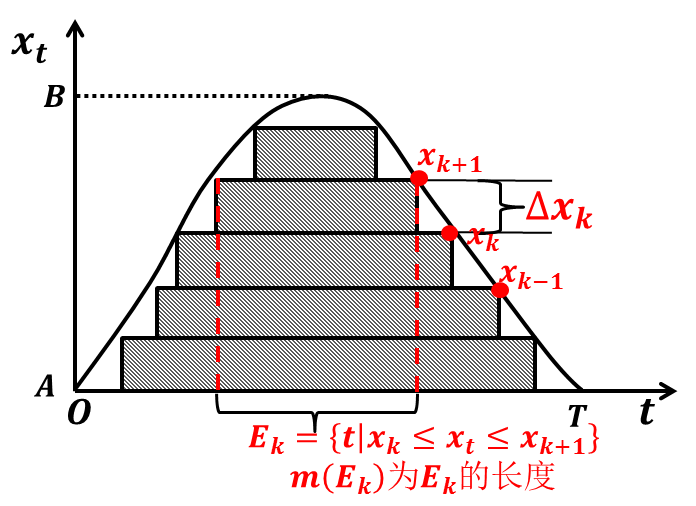
\includegraphics[width=\textwidth]{images/L_Integral.jpg}
                \caption{L积分示意图}
                \label{fig:L积分示意图}
                \end{subfigure}
            \qquad
                \begin{subfigure}[b]{0.3\textwidth}
                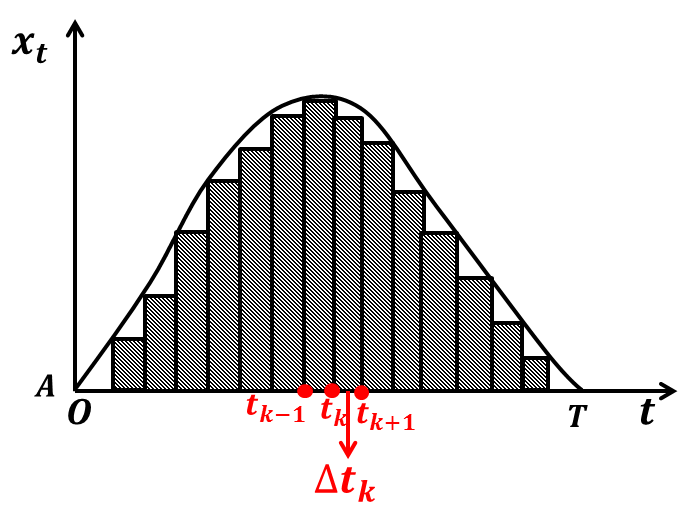
\includegraphics[width=\textwidth]{images/R_Integral.jpg}
                \caption{R积分示意图}
                \label{fig:R积分示意图}
                \end{subfigure}
            \caption{L积分和R积分对比示意图}
            \label{fig:L积分和R积分对比示意图}
            \end{figure}

%           %%%%这个地方有个图片
            % \textcolor[rgb]{1 0 0}{todo:图片:L积分和R积分对比示意图}
            \par
            设$E = [0,T] \subset R$是可测集,且$E$的长度$m(E)$有界,$m(E)<\infty$,$x_t$是$E$上的可测函数(或者有界函数),记函数$x_t$在域$E$上的界$x_t(E)$为$M,N$,即$M \leqslant x_t(E) \leqslant N$,下面,我们在域$E$上介绍函数$x_t$的勒贝格积分。\\
            \textbf{Step1.}划分$n$段。我们将界$[M,N]$离散化为$n$段,有
            \begin{align*}
                M = x_0 <\dots <x_k < x_{k+1} <\dots<x_n = N
            \end{align*}
            并且记分割方法为$A = \{x_k\}^n$,
            记第$k$段的长度为$\Delta x_k = x_{k+1}-x_k,k = 0,1,\dots,n - 1$,当然,也可以写为$\Delta x_k = x_{k}-x_{k-1},k = 1,2,\dots,n$,不过一定要注意下标别混乱了。记$n$个小段的最大长度为$\delta$
            \begin{align*}
                \delta = \max_{0 \leqslant k \leqslant n-1}\{\Delta x_k\}
            \end{align*}
            为了简便,我们将其简单的均分$n$段。\\
            \textbf{Step2.}取点$\xi_k$。在第$k$段$[x_{k},x_{k+1}]$中任取一点$\xi_k\in [x_{k},x_{k+1}]$,则其对应的自变量集为$E_k$,$E_k = \{t|x_k \leqslant x_t \leqslant x_{k+1}\}$,且$E_k$的长度为$m(E_k)$。\\
            \textbf{Step3.}计算勒贝格积分
            \begin{align*}
                \int_0^T x_t\mathrm{d}t = \lim_{\delta \rightarrow 0} \sum_{k = 0}^{n-1} \xi_k m(E_k)
            \end{align*}
            \textbf{Step4.}L可积。若在$\delta\rightarrow 0$时,极限
            \begin{align*}
                \lim_{\delta \rightarrow 0} \sum_{k = 0}^{n-1} \xi_k m(E_k) = L<\infty
            \end{align*}
            存在,且$L$与分割方法$A$无关,与取点$\{\xi_k\}$点无关,则称$x_t$在区间$E = [0,T]$上勒贝格可积,$L$为其黎曼积分。\\
            注:$L^p(\Omega)$为$\Omega$上L可积的函数集;$C_0^\infty$为L可积且光滑的函数集。勒贝格积分的性质如下:\\
            1).R可积必L可积,且二者积分值相等;\\
            2).线性性和可加性;\\
            3).绝对值不等式
            \begin{align*}
                \left| \int_E f\mathrm{d}m \right| \leqslant \int_E |f| \mathrm{d}m
            \end{align*}
        \subsubsection{积分号下取极限}
            \label{subsubsec:积分号下取极限}
            \par
            在前面的随机过程中,我们提到过样本路径$X(t,w)$(或者写为$X_t(w)$)是随机过程$X_t$的一次样本实现。现在,不妨想象我们有$n$次样本实现,于是,我们就有$n$个样本路径$X_n(t,w)$,当然,我们可以将$n$次样本实现绘成图像。再考虑一个问题,我们“放弃”随机,不妨考虑普通函数$x_t$,如果用$x_n(t)$来做函数$x_t$的逼近(这可以是函数估计,函数逼近和ODE等等问题),我们会使函数列$\{x_n(t)\}$尽可能逼近目标函数$x_t$,如图(\ref{fig:函数列逼近函数示意图})所示
            \begin{figure}[H]
                \centering
                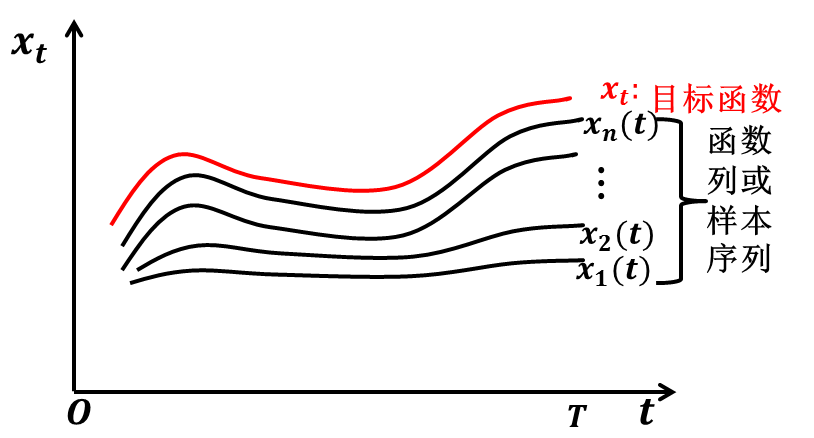
\includegraphics[height=3cm]{images/func_to_func.jpg}
                \caption{函数列逼近函数示意图}
                \label{fig:函数列逼近函数示意图}
            \end{figure}
            %%%%这个地方有个图片
            % \textcolor[rgb]{1 0 0}{todo:图片:函数列逼近函数示意图}
            \par
            在用函数列$\{x_n(t)\}$逼近$x_t$时,我们对$x_t$求积分,如果
            \begin{align*}
                \lim_{n \rightarrow \infty} x_n(t) = x_t
            \end{align*}
            那么,我们很希望有下面的情况(积分与极限可以互换位置)
            \begin{align*}
                \lim_{n \rightarrow \infty} \int_0^T x_n(t) \mathrm{d}t = \int_0^T \lim_{n \rightarrow \infty}x_n(t) \mathrm{d}t = \int_0^T x_t \mathrm{d}t
            \end{align*}
            \par
            然而,上面的积分与极限互换位置不是随便就能发生的。在R积分中,只有当函数列$\{x_n(t)\}$一致收敛于$x_t$时,我们才能将积分与极限互换位置,这对函数列$\{x_n(t)\}$提出了很高的要求;在L积分中,这种要求相对弱一些,有如下的勒贝格控制收敛定理
            \begin{theorem}[勒贝格控制收敛定理]
            $E$为可测集,$m(E)<\infty$,$\{x_n(t)\}$是$E$上有界可测函数列,并且满足:\\
            1.$\{x_n(t)\}$在$E$上几乎处处收敛于$x_t$
            \begin{align*}
                \lim_{n \rightarrow \infty} x_n(t) = x_t \quad a.e\text{于}E
            \end{align*}
            2.存在$E$上L可积函数$g(t)$,在$E$上有$|x_n(t) |\leqslant g(t)$,$a.e$于$E$。这里$g(t)$是控制函数,可以是非负可测函数。\\
            则$x_t$在$E$上L可积,并且
            \begin{align*}
                \int_E x_td_t = \int_E \lim_{n \rightarrow \infty}x_n(t) \mathrm{d}t = \lim_{n\rightarrow \infty} \int_Ex_n(t) \mathrm{d}t
            \end{align*}
            \end{theorem}
            \par
            用数学语言描述勒贝格控制收敛定理为:$L$为可测集$E$上L可积函数集(有界可测)。设$x_n(t)\in L,x_n(t)\xrightarrow{a.e}x_t$,若$\exists g\in L,\forall n \geqslant 1$,有$|x_n(t) \leqslant g|,a.e$,则$x_t\in L$且
            \begin{align*}
                \lim_{n\rightarrow \infty} \int_Ex_n(t) \mathrm{d}t = \int_E x_td_t
            \end{align*}
            \begin{lemma}[Fatou引理]
            $\{x_n(t)\}$为可测集$E$上的非负可测函数列,且$x_n(t)\xrightarrow{a.e}x_t$,则有
            \begin{align*}
                \int_E x_t \mathrm{d}t \leqslant \sup_{n \geqslant 1}\left\{ \int_E x_n(t) \mathrm{d}t\right\}
            \end{align*}
            \end{lemma}
            \begin{lemma}[Levi引理]
            设$x_1(t) \leqslant x_2(t) \leqslant \dots \leqslant x_n(t) \leqslant \dots$是定义在可测集$E$上的非负可测函数列,且$x_n(t)\xrightarrow{a.e}x_t$,则有
            \begin{align*}
            \int_E x_t \mathrm{d}t  = \lim_{n \rightarrow \infty} \int_E x_n(t) \mathrm{d}t = \int_E \lim_{n \rightarrow \infty} x_n(t) \mathrm{d}t
            \end{align*}
            \end{lemma}
            注:上面的积分中要求$E$有界,$x_t$有界,后续可推广到$\infty$。上述定理更准确的数学定义参考《测度论讲义》严加安P50-P54。

        \subsubsection{黎曼-斯蒂尔切斯积分}
            \label{subsubsec:黎曼-斯蒂尔切斯积分}
            \par
            黎曼-斯蒂尔切斯积分(Riemann-Stieltjes积分,简称R-S积分),其实在前面试解$\int_0^T W_t\mathrm{d}W_t$时,我们已经初见R-S的身影。R-S积分是将R积分在Stielejes下进行推广的,将R积分$\int f\mathrm{d}x = \sum f \Delta x$推广到$\int f\mathrm{d}g(x) = \sum f \Delta g(x)$,例如
            \begin{align*}
                \int_0 ^T x_t \mathrm{d} w_t = \sum_{k = 0}^{n-1} x(\tau_k) [w(t_{k+1}) - w(t_k)]
            \end{align*}
            其中:$x_t,w_t$是普通函数,而非随机过程。\\
            \textbf{Step1.}划分$n$段。我们将区间$[0,T]$离散化为$n$段,有
            \begin{align*}
                0 = t_0 <\dots <t_k < t_{k+1} <\dots<t_n = T
            \end{align*}
            并且记分割方法为$A = \{t_k\}^n$,
            记第$k$段的长度为$\Delta x_k = x_{k+1}-x_k,k = 0,1,\dots,n - 1$,
            记$n$个小段的最大长度为$\delta$
            \begin{align*}
                \delta = \max_{0 \leqslant k \leqslant n-1}\{\Delta x_k\}
            \end{align*}
            \textbf{Step2.}取点$\tau_k$。在第$k$段$[t_{k},t_{k+1}]$中任取一点$\tau_k\in [t_{k},t_{k+1}]$,则该点的函数值为$x(\tau_k)$。\\
            \textbf{Step3.}计算$\Delta w(x_k)$ 。
            \begin{align*}
            \Delta w(x_k) = w(t_{k+1}) - w(t_k)
            \end{align*}
            \textbf{Step4.}计算R-S积分
            \begin{align*}
                \int_0^T x_t\mathrm{d}w_t = \lim_{\delta \rightarrow 0} \sum_{k = 0}^{n-1} x(\tau_k)\Delta w(x_k)
            \end{align*}
            \textbf{Step5.}R-S可积。若在$\delta\rightarrow 0$时,极限
            \begin{align*}
                \lim_{\delta \rightarrow 0} \sum_{k = 0}^{n-1} x(\tau_k)\Delta w(x_k) = R<\infty
            \end{align*}
            存在,且极限值$R$与分割方法$A$无关,与$\{\tau_k\}$无关,则称$x_t$关于$w_t$在区间$[0,T]$上的R-S积分存在且R为其积分值。
            \par
            R-S积分存在的充分条件为:函数$x_t$连续,$w_t$单调。上面定义的积分界$[0,T]$有界,我们可以将它推广到无限区间$[0,\infty]$上
            \begin{align*}
            \int_0^\infty x_t\mathrm{d}w_t = \lim_{T \rightarrow \infty} \int_0^T x_t\mathrm{d}w_t
            \end{align*}
            此外,R-S积分也有一些性质,这里不做讨论。

        \subsubsection{Ito积分}
            \label{subsubsec:Ito积分}
            前面讨论的R积分、L积分和R-S积分中的函数$x_t,w_t$都是普通函数,而非随机过程。下面将函数引入到随机过程当中,仍然用大写的$X_t,W_t$来表示随机过程。考虑如下积分形式
            \begin{align*}
                \int_0^T X_t \mathrm{d}W_t
            \end{align*}
            \par
            \ding{172}先假设$X_t$为普通函数$x_t$,$W_t$为Brown运动,且$x_t$不依赖与$W_t$,于是,经过划分、取点、求积等过程,我们可以定义其积分形式为
            \begin{align*}
                \int_0^T x_t \mathrm{d}W_t = \sum_{k = 0}^{n - 1} x(\tau_k)[W(t_{k+1}) - W(t_k)]
            \end{align*}
            \par
            可以定义$\Delta W_k = W(t_{k+1}) - W(t_k)$。由于Brown运动的正态增量的性质$W(t) - W(s) \sim N(0,t-s)$,所以上式定义的积分是一个服从高斯分布的随机变量,且其均值为
            \begin{align*}
                &E\left(\int_0^T x_t \mathrm{d}W_t\right) \\
                ={}& E\left( \sum_{k = 0}^{n - 1} x(\tau_k)[W(t_{k+1}) - W(t_k)] \right) \\
                ={}& 0
            \end{align*}
            其方差为
            \begin{align*}
                &Var\left(\int_0^T x_t \mathrm{d}W_t\right) \\
                ={}& Var\left( \sum_{k = 0}^{n - 1} x(\tau_k)[W(t_{k+1}) - W(t_k)] \right) \\
                ={}& \sum_{k = 0}^{n-1}x(\tau_k)^2 (t_{k+1} - t_k)
            \end{align*}
            \par
            \ding{173}先将$X_t$视为简单的随机过程(例如:$X_t$在各个时间段$[t_k,t_{k+1}]$为随机变量$\xi_k$,并且各个时刻之间的随机变量毫不相关),
            经过划分、取点、求积等过程,我们可以定义其积分形式为
            \begin{align*}
                \int_0^T X_t \mathrm{d}W_t = \sum_{k = 0}^{n - 1} X(\tau_k)[W(t_{k+1}) - W(t_k)]
            \end{align*}
            因为$X_t$是一个简单的随机过程,则$X(\tau_k)$可以记为一个简单的随机变量$\xi_k$,$\xi_k$依赖于$W_t(t \leqslant t_k)$,但不依赖于$W_t(t>t_k)$,由此,其积分形式还可以写为
            \begin{align*}
                \int_0^T X_t \mathrm{d}W_t = \sum_{k = 0}^{n - 1} \xi_k [W(t_{k+1}) - W(t_k)]
            \end{align*}
            上面定义的这个积分具有以下性质:\\
            1.线性性。设$X_t,Y_t$为简单的随机过程,有
            \begin{align*}
                \int_0^T [\alpha X_t + \beta Y_t] \mathrm{d}W_t = \alpha \int_0^TX_t\mathrm{d}W_t + \beta \int_0^TY_t\mathrm{d}W_t
            \end{align*}
            2.零均值性。如果$E[\xi_i^2]<\infty,(k = 0,1,\dots,n-1)$,则
            \begin{align*}
                E\left[ \int_0^T X_t \mathrm{d}W_t\right] = 0
            \end{align*}
            3.等距性。如果$E[\xi_i^2]<\infty,(k = 0,1,\dots,n-1)$,则
            \begin{align*}
            E\left[ \int_0^T X_t \mathrm{d}W_t\right]^2 =\int_0^T E\left[ X_t^2 \right]\mathrm{d}t
            \end{align*}
            \par
            \ding{174}现在将$X_t$扩展到更广泛的随机过程(注意:$X_t$即为随机微分方程的解)。为了方便讨论,我们给$X_t$规定一个随机过程类$V$,在定义随机过程类之前,我们先给出适应过程的定义:
            \begin{definition}[适应过程]
            设$\{X_t\}$是一个随机过程,$\{\mathcal{F}_t\}$是$\sigma$代数流。若对$\forall t$,$x_t$是$\mathcal{F}_t$可测的,则称$\{X_t\}$是$\{\mathcal{F}_t\}$适应过程。
            \end{definition}
            \par
            下面,我们来定义一个随机过程类$V$
            \begin{align*}
                V = \left\{X_t\biggl|X_t\text{是}[0,T]\text{上可测适应过程,满足}E\left[ \int_0^T X_t^2 \right] < \infty\right\}
            \end{align*}
            进一步,定义
            \begin{align*}
                V^* = \left\{X_t\biggl|X_t\text{是}[0,T]\text{上可测适应过程,且}\forall T>0,\text{满足} \int_0^T X_t^2 < \infty ,a.s\right\}
            \end{align*}
            注:$a.s$表示几乎必然收敛(以概率$1$收敛),英文为$almost\ sure$。
            \begin{definition}[Ito积分]
            设$X_t\in V(0,T)$,$X_t$的积分可以定义为
            \begin{align*}
                \int_0^T X(t,w) \mathrm{d}W_t = \lim_{n \rightarrow \infty}\int_0^T \phi_n(t,w)\mathrm{d}W_t \quad \in L^2(P)
            \end{align*}
            其中:$L^2(P)$表示$P$上平方$L$可积函数集;$\{\phi_n(t)\}$是初等随机过程序列,且当$n\rightarrow \infty$时,有
            \begin{align*}
                E\left\{ \int_0^T [X(t,w) - \phi_n(t,w)]^2 \mathrm{d}t\right\} \rightarrow 0
            \end{align*}
            上面定义的积分形式即为Ito积分。
            \end{definition}
            \par
            关于Ito积分中的初等随机序列$\{\phi_n\}$的构造,可以查阅《随机微分方程及其在数理金融中的应用》蒲兴成P16-P17。在实际问题中,我们遇到的过程常常不在随机过程类$V$中,为此,我们可以将Ito积分推广到$V^*$函数类。

        \subsubsection{Ito积分的性质}
            \par
            上面给出了Ito积分的定义,下面,我们来介绍Ito积分的一些性质:
            1.可加性;
            2.线性性;
            3.对任意固定的$T0$,随机过程$X_t$的Ito积分$\int_0^T X_t \mathrm{d}W_t$是一个随机变量(其实,不仅仅是Ito积分,任何带有随机性$\mathrm{d}W_t$的积分都是一个随机变量);
            4.零均值性。
            \begin{align*}
                E\left[ \int_0^T X_t \mathrm{d}W_t\right] = 0
            \end{align*}
            \begin{lemma}[Ito引理]
            $\forall X_t \in V(0,T)$,有
            \begin{align*}
                E\left[ \left( \int_0^T X(t,w) \mathrm{d}W_t \right)^2 \right] =
                E\left[  \int_0^T X(t,w)^2 \mathrm{d}t \right]
            \end{align*}
            \end{lemma}
            \par
            下面来看一下随机过程的逼近情况:若$X(t,w)\in V,X_n(t,w)\in V$,且当$n\rightarrow \infty$时,有
            \begin{align*}
                E\left[ \int_0^T ( X_n(t,w) - X(t,w) )^2\mathrm{d}t \right] \rightarrow 0
            \end{align*}
            则有
            \begin{align*}
                \int_0^T X_n(t,w) \mathrm{d}W_t \rightarrow \int_0^T X(t,w) \mathrm{d}W_t \quad \in L^2(P)
            \end{align*}
            \par
            在上面的性质中,我们知道,对任意固定的$T0$,随机过程$X_t$的Ito积分$\int_0^T X_t \mathrm{d}W_t$是一个随机变量,由随机变量,我们就可以再构造一个随机过程。我们定义一个新的随机过程
            \begin{align*}
                Y_t = \int_0^t X_s \mathrm{d}W_s
            \end{align*}
            其中:$t\in [0,T]$,$s\in [0,t]$。我们称随机过程$Y_t$是Ito积分过程,可以发现,前面的随机微分方程
            \begin{align*}
                X_t = X_0+\int_0^t f(s,X_s) \mathrm{d}s+ \int_0^t g(s,X_s) \mathrm{d}W_s
            \end{align*}
            的解$X_t$其实就类似一个Ito积分过程。可以证明,Ito积分过程$Y_t$存在连续的样本路径,下面,我们来讨论一下随机过程$Y_t$的随机性质。
            \begin{theorem}[鞅性质]
            设$X_t\in V^*$,且$\int_0^\infty E[X_t^2]\mathrm{d}t < \infty$,则
            \begin{align*}
                Y_t = \int_0^t X_s\mathrm{d}W_s \quad 0 \leqslant t \leqslant T
            \end{align*}
            是一个零均值的连续平方可积鞅(过程)。
            \end{theorem}
            \begin{definition}[Gauss过程]
            如果$X_t$非随机,且$\int_0^T X_t^2 \mathrm{d}t < \infty$,则对$\forall t$
            \begin{align*}
                Y_t = \int_0^t X_s\mathrm{d}W_s
            \end{align*}
            是一个服从正态分布的随机变量。如果$t\in [0,T]$,,则随机过程$\{Y_t\}$是一个Gauss过程,其均值函数为常值$0$,协方差函数为
            \begin{align*}
                Cov[Y_t,Y_{t+u}] = \int_0^t X_s^2 \mathrm{d}s ,\quad u \geqslant 0
            \end{align*}
            \end{definition}

    \subsection{Ito过程与Ito公式}
        \label{subsec:Ito过程与Ito公式}
        \subsubsection{Ito过程}
            \label{subsubsec:Ito过程}
            \par
            在前面随机积分的初步尝试部分,我们讨论了Brown运动的二次变差(\ref{Brown运动的二次变差})。Brown运动$W_t$在时间区间$[0,t]$上的二次变差为$t$,即
            \begin{align*}
                [W,W](t) = \lim_{\delta_n \rightarrow 0} \sum_{k = 0}^{n - 1} |W(t_{k+1}) - W(t_k)|^2 = t
            \end{align*}
            其中:$\{t_k\}$为$[0,t]$上的$n$段分割,$\delta_n = \max\limits_{0 \leqslant k \leqslant n-1}\{t_{k+1} - t_k\}$。上式从形式上可以表示为
            \begin{align*}
                \int_0^t [\mathrm{d}W_s]^2 = \int_0^t \mathrm{d}s= t
            \end{align*}
            或者
            \begin{align*}
                [\mathrm{d}W_t]^2 = \mathrm{d}t
            \end{align*}
            更常见的写法是
            \begin{align}
                \label{Wt差分的计算公式}
                \mathrm{d}W_t \approx \sqrt{\mathrm{d}t}
            \end{align}
            更一般的,我们有下面定理
            \begin{theorem}
                设$x$是有界连续函数,$\{t_k\}$为$[0,t]$上的$n$段分割,则$\forall \theta_k \in [W(t_{k+1}),W(t_k)]$,依概率收敛意义下的极限
                \begin{align*}
                    \lim_{\delta_n \rightarrow 0} \sum_{k = 0}^{n - 1} x(\theta_k) [W(t_{k+1}) - W(t_k)]^2 = \int_0^t x[W_s]\mathrm{d}s
                \end{align*}
            \end{theorem}
            \par
            前面,我们简单的介绍了Ito积分过程,下面,我们给出Ito过程的定义:
            \begin{definition}[Ito过程]
                设$W_t$表示一维Brown运动,如果一个一维的过程$X_t$可以表示成一个随机积分
                \begin{align*}
                    X_t = X_0 +\int_0^t \mu(s)\mathrm{d}s + \int_0^t \sigma(s) \mathrm{d}W_s
                \end{align*}
                或者随机微分方程
                \begin{align*}
                    \left\{
                        \begin{aligned}
                            &\mathrm{d}X_t = \mu(t)\mathrm{d}t + \sigma(t) \mathrm{d}W_t\\
                            &X(t_0) = X_0
                        \end{aligned}
                    \right.
                \end{align*}
                并且过程$\mu(t),\sigma(t)$满足:\\
                1.$\mu(t)$是适应的,并且满足
                \begin{align*}
                    \int_0^T |\mu(t)|\mathrm{d}t < \infty,\quad a.s
                \end{align*}
                2. $\sigma(t)\in V^*$;\\
                则称$X_t$是一个Ito过程。
            \end{definition}
            \par
            由Ito过程的定义可以看出,前面要求解的人口增长随机微分方程的解$X_t$是一个Ito过程。值得一提的是,并不是所有的随机微分方程都是Ito过程,对许许多多的SDE,我们都无法求出其解析解。
        \subsubsection{Ito公式}
            \label{subsubsec:Ito公式}
            \par
            上面的内容介绍了Ito积分的定义、Ito积分的性质并介绍了Ito过程。但是如果我们仅根据定义来计算Ito积分的话,那就太麻烦了,那么Ito积分有没有积分公式呢?像R积分中有牛顿—莱布尼茨共识那样,有的。下面,我们就来介绍Ito积分的计算公式—Ito公式(非线性链式法则)
            \begin{theorem}[Ito公式]
                设$X_t$是一个Ito过程
                \begin{align*}
                    \mathrm{d}X_t = \mu(t )\mathrm{d}t+\sigma(t)\mathrm{d}W_t
                \end{align*}
                $g(t,x)\in C^2[R^+\times R]$(即$g$是$[0,+\infty)\times R$上的二次连续可微函数),则
                \begin{align*}
                Y_t = g(t,X_t)
                \end{align*}
                仍是一个Ito过程,且
                \begin{align}
                    \label{Ito公式}
                    \mathrm{d}Y_t = \frac{\partial g}{\partial t}(t,X_t)\mathrm{d}t +\frac{\partial g}{\partial x}(t,X_t )\mathrm{d}X_t + \frac{1}{2} \frac{\partial^2 g}{\partial x^2}(t,X_t)\cdot
                    \mathrm{d}(X_t)^2
                \end{align}
                其中:$\mathrm{d}(X_t)^2 = \mathrm{d}(X_t)\cdot \mathrm{d}(X_t)$是按照如下规则计算的
                \begin{align}
                    \label{Ito公式微分计算}
                    \left\{
                        \begin{aligned}
                        &\mathrm{d}t\cdot\mathrm{d}t = \mathrm{d}t \cdot \mathrm{d}W_t = \mathrm{d}W_t \cdot \mathrm{d}t  =0\\
                        &\mathrm{d}W_t \cdot\mathrm{d}W_t = \mathrm{d}t
                        \end{aligned}
                    \right.
                \end{align}
            \end{theorem}
            \begin{Proof}
                利用式(\ref{Ito公式微分计算})有
                \begin{align*}
                    g(t,X_t) &= g(0+X_0)+\int_0^t\left[ \frac{\partial g}{\partial s}(s,X_s) +\mu_s \frac{\partial g}{\partial x}(s,X_s) + \frac 12 \sigma_s^2 \cdot \frac{\partial^2 g}{\partial x^2}(s,X_s)\right] \mathrm{d}s \\
                    &\quad +\int_0^t\sigma_s \cdot \frac{\partial g}{\partial x}(s,X_s) \mathrm{d}W_s
                \end{align*}
                其中:$\mu_s = \mu(s,w),\sigma_s = \sigma(s,w)$。我们可以知道$g(t,X_t)$是一个随机过程。为简单,设$g,\frac{\partial g}{\partial t},\frac{\partial g}{\partial x},\frac{\partial^2 g}{\partial x^2}$是有界的,能够证明,在此情况下可以在$C^2$中构建一个函数列$g_n$,使得当$n\rightarrow \infty$时,$g_n,\frac{\partial g_n}{\partial t},\frac{\partial g_n}{\partial x},\frac{\partial^2 g_n}{\partial x^2}$在$[0,\infty)\times R$的紧子集中分别一致趋近于$g,\frac{\partial g}{\partial t},\frac{\partial g}{\partial x},\frac{\partial^2 g}{\partial x^2}$。此外,我们可以假定$\mu(t,w),v(t,w)$是初等函数。利用泰勒展开,有
                \begin{align*}
                    g(t,X_t) &= g(0,X_0) + \sum_j\Delta g(t_j,X_j)\\
                    & = g(0,X_0)+\sum_j \frac{\partial g}{\partial t}\Delta t_j +\sum_j\frac{\partial g}{\partial x}\Delta X_j + \frac 12 \sum_j \frac{\partial^2 g}{\partial t^2}(\Delta t_j)^2\\
                    & \quad + \sum_j \frac{\partial^2 g}{\partial t \partial x}(\Delta t_j)(\Delta X_j) + \frac 12 \frac{\partial^2 g}{\partial x^2}(\Delta X_j)^2 + \sum R_j
                \end{align*}
                其中:
                \begin{align*}
                &\Delta t_j = t_{j+1} - t_j ,\Delta X_j = X_{t_{j+1}} - X_{t_j},\\
                &\Delta g(t_j,X_j) = g(t_{j+1},X_{t_{j+1}}) - g(t_j,X_{t_j}),R_j = O (|\Delta t_j|^2 +|\Delta X_j|^2)
                \end{align*}
                则当$\Delta t_j \rightarrow 0$时,有
                \begin{align*}
                    \sum_j \frac{\partial g}{\partial t}\Delta t_j = \sum_j \frac{\partial g}{\partial t}(t_j,X_j)\Delta t_j \rightarrow \int_0^t\frac{\partial g}{\partial t}(s,X_s) \mathrm{d}s\\
                    \sum_j \frac{\partial g}{\partial x}\Delta X_j = \sum_j \frac{\partial g}{\partial x}(t_j,X_j)\Delta X_j \rightarrow \int_0^t\frac{\partial g}{\partial x}(s,X_s) \mathrm{d}X_s
                \end{align*}
                此外,因为$\mu,\sigma$是初等函数,所以有
                \begin{align}
                    \label{Ito公式证明2}
                    \sum_j \frac{\partial^2 g}{\partial x^2}(\Delta X_j)^2 &= \sum_j\frac{\partial^2 g}{\partial x^2}\mu_j^2(\Delta t_j)^2 + 2\sum_j \frac{\partial ^2 g}{\partial x^2} \mu_j\sigma_j(\Delta t_j)(\Delta W_j) \notag\\
                    & \quad + \sum_j \frac{\partial ^2g}{\partial x^2} \sigma_j^2 \cdot (\Delta W_j)^2
                \end{align}
                其中:$\mu_j = u(t_j,w),\sigma_j = \sigma(t_j,w)$。易证在$\Delta t_j \rightarrow 0$时,上式(\ref{Ito公式证明2})中的前两项都趋近于$0$,例如
                \begin{align*}
                    &\lim_{\Delta t_j \rightarrow 0} E \left[ \left( \sum_j \frac{\partial ^2 g}{\partial x^2} \mu_j\sigma_j(\Delta t_j)(\Delta W_j) \right) ^2\right] \\
                    ={}& \lim_{\Delta t_j \rightarrow 0} E \left[ \left( \sum_j \frac{\partial ^2 g}{\partial x^2} \mu_j\sigma_j \right) ^2\right](\Delta t_j)^3 \\
                    ={}& 0
                \end{align*}
                下面证明,当$\Delta t_j \rightarrow 0$时,在$L^2(P)$中式(\ref{Ito公式证明2})的最后一项趋于$\int_0^t\frac{\partial^2g}{\partial x^2}\sigma^2\mathrm{d}s$。为证明这一点,记
                \begin{align*}
                a(t) = \frac{\partial^2g}{\partial x^2}(t,X_t)\sigma^2(t,w),\quad a_j = a(t_j)
                \end{align*}
                因为
                \begin{align*}
                    E\left[ \left( \sum_j a_j(\Delta W_j)^2 - \sum_ja_j\Delta t_j\right)^2 \right] = \sum_{i,j}E[a_ia_j((\Delta W_j)^2 - \Delta t_j)]
                \end{align*}
                且当$i<j$时,$a_ia_j((\Delta W_j)^2 - \Delta t_j)$与$(\Delta W_j)^2 - \Delta t_j$是独立的,因而此时这项可以忽略。类似的,当$i>j$时,有
                \begin{align*}
                    &\lim_{\Delta t_j \rightarrow 0} \sum_jE [(a_j)^2((\Delta W_j)^2 - \Delta t_j)^2]\\
                    ={}&\lim_{\Delta t_j \rightarrow 0} \sum_jE[a_j^2]\cdot E[(\Delta W_j)^4 - 2(\Delta W_j)^2 \Delta t_j + (\Delta t_j)^2]\\
                    ={}&\lim_{\Delta t_j \rightarrow 0} \sum_jE[a_j^2]\cdot [3(\Delta t_j)^2 - 2(\Delta W_j)^2 \Delta t_j + (\Delta t_j)^2]\\
                    ={}&\lim_{\Delta t_j \rightarrow 0} \sum_jE[a_j^2]\cdot (\Delta t_j)^2\\
                    ={}& 0
                \end{align*}
                即在$L^2(P)$中,有
                \begin{align*}
                    \lim_{\Delta t_j \rightarrow 0} E\left[ \sum_j a_j (\Delta W_j)^2 \right] = \int_0^ta(s)\mathrm{d}s
                \end{align*}
                上式通常写为$(\mathrm{d}W_t)^2 = \mathrm{d}t$。类似上面的讨论,同样可以证明:$\lim_{\Delta t_j \rightarrow 0} R_j = 0$。综上所述,Ito公式成立。$\square$
            \end{Proof}
            \par
            上面介绍了Ito公式,下面我们就用Ito公式来求解前面建立的人口增长的随机微分方程模型(\ref{被规范的方程}),由
            \begin{align*}
                \frac{\mathrm{d}X_t }{X_t} = r\mathrm{d}t + \mathrm{d}W_t
            \end{align*}
            对上式积分,有
            \begin{align*}
                \int_0^t \frac{\mathrm{d}X_s}{X_s} = rt+W_t \quad (W_0 = 0)
            \end{align*}
            为计算左边积分,对函数$g(t,x) = \ln x(x>0)$运用Ito公式,有
            \begin{align*}
                \mathrm{d}(\ln X_t) &= \frac{1}{X_t} \cdot \mathrm{d}X_t + \frac 12\left(- \frac{1}{X_t^2} \right) (\mathrm{d}X_t)^2\\
                &=\frac{\mathrm{d}X_t}{X_t} - \frac{1}{2X_t} \cdot X_t^2 \mathrm{d}t \\
                & = \frac{\mathrm{d}X_t}{X_t} -\frac{1}{2} \mathrm{d}t
            \end{align*}
            所以
            \begin{align*}
                \frac{\mathrm{d}X_t }{X_t} = \mathrm{d}(\ln X_t) + \frac 12 \mathrm{d}t
            \end{align*}
            代入所求方程,有
            \begin{align*}
                \ln \frac{X_t}{X_0} = \left( r - \frac 12 \right)t + W_t
            \end{align*}
            或者
            \begin{align*}
                X_t = X_0 \exp \left[\left( r - \frac 12 \right)t + W_t\right]
            \end{align*}

    \subsection{解的存在唯一性及解析计算公式}
        \label{subsec:解的存在唯一性及解析计算公式}
        \subsubsection{解的存在唯一性}
            \label{subsubsec:解的存在唯一性}
            \par
            现在,回到标准随机微分方程模型当中(\ref{规范的方程}),对于一个SDE问题,我们基本的目标就是求解方程的解析解或者数值解,在有解之后再来了解一下解的性质。对于SDE的解,我们已经知道其解是一个随机过程。在对前面ODE和PDE解的分析中,我们讨论了解的定义、解的存在唯一性、解的解析求法、解的数值求法和解的稳定性,那么,对SDE的解,我们仍旧要讨论上面的问题(前面我们已经给出SDE解的定义)。首先,我们来讨论解的存在唯一性,我们并不打算直接在SDE一般形式下讨论
            \begin{align*}
                \mathrm{d}X_t = f(X_t,W_t,t)
            \end{align*}
            那样太过于泛化。我们来讨论Ito型随机微分方程的解的存在唯一性(Stratonovich型随机微分方程等其他形式这里不做讨论)。前面已经介绍过Ito型随机微分方程(\ref{随机微分方程的一般形式}),这里再重写一下
            \begin{align*}
                \left\{
                    \begin{aligned}
                            &\mathrm{d}X_t = f(X_t,t)\mathrm{d}t + g(X_t,t)\mathrm{d}W_t \quad t\in [t_0,T]\\
                            &X_{t_0} = X_0
                    \end{aligned}
                \right.
            \end{align*}
            Ito型随机积分方程为
            \begin{align*}
                X_t = X_0+\int_0^t f(s,X_s)\mathrm{d}s + \int_0^t g(s,X_s)\mathrm{d}W_s
            \end{align*}
            \par
            下面规范一下上式的1.量空间、2.映射空间、3.解域。$t\in [0,T]$;$X_0\in R$可以是常量,也可以是一随机变量,但要求其平方可积$E[|X_0|^2]<\infty$;
            $W_t\in R$是一个Brown运动。既然有随机,我们定义一个概率空间$(\Omega,\mathcal{F},P)$,$W_t$是概率空间$(\Omega,\mathcal{F},P)$上的Brown运动,$\{\mathcal{F}_t\}$是$W_t$产生的$\sigma$代数流;
            $f(X_t,t):R\times [0,T] \rightarrow R$;
            $g(X_t,t):R\times [0,T] \rightarrow R$。
            \par
            上面只给出了映射$f,g$的量变换,并没有给出$f,g$的类型,我们要求$f,g$是$[0,T]$上的(Borel)连续可测函数,并且要求$f,g$满足Ito过程的要求,即\\
            1).$f(X_t,t)$是适应的并且$\int_0^T |f(X_t,t)|\mathrm{d}t < \infty,a.s$;\\
            2).$g(X_t,t)\in V^*$。
            \par
            上述Ito型随机微分方程可能存在两种形式的解:\ding{172}给定$f,g$,解(过程)$X_t$依赖于时间$t$
            与$W_t$在$[0,t]$的值有关,显然$X_t$是强吻合上述方程的,故称$X_t$为强解;\ding{173}给定$f,g$,$X_t$不依赖与时间$t$,仅与$W_t$的前值有关,这样的解$X_t$称为弱解,不妨记为$\tilde{X}_t$,$\tilde{X}_t$并不完全吻合随机方程。下面,我们给出Ito型随机微分方程强解的存在唯一性定理:
            \begin{theorem}[强解的存在唯一性]
                设$f(t,x),g(t,x)$是$[0,T]\times R$上的(Borel)可测函数且$|f(t,x)|^{\frac 12},|g(t,x)|$平方可积。如果$f,g$满足:\\
                1.(Lipschitz条件)$\exists L >0$,$\forall t\in [0.T]$,使得$\forall x,y \in R$,有
                \begin{align*}
                    |f(t,x) - f(t,y) | \leqslant L|x-y|\\
                    |g(t,x) - g(t,y) | \leqslant L|x-y|
                \end{align*}
                2.(线性增长条件)$\exists K > 0$,使得$\forall t\in [0,T],x\in R$,有
                \begin{align*}
                    |f(t,x)|+ |g(t,x)|\leqslant K(1+|x|)
                \end{align*}
                并且,初始值$X_0$独立于由$\{W_s,s \geqslant 0\}$产生的$\sigma$代数$\{\mathcal{F}_t\}$,且$E[|X_0|^2]<\infty$,则Ito型随机微分方程存在唯一解$X_t$,并且解的路径$X_t(w)$连续,还有$X_t$适应于由$X_0$和$\{W_s,s \leqslant t\}$产生的流域$\{\mathcal{F}_t\}$,并且$E\int_0^T|X_t|^2\mathrm{d}t < \infty$。
            \end{theorem}
            注:上述证明可以参考《Stochastic\ Differential\ Equations》B.Qksendal;或者《随机微分方程及其在数理金融中的应用》蒲兴成P37-P40。
        \subsubsection{解析计算公式}
            \label{subsubsec:解析计算公式}
            \par
            在SDE存在唯一解的情况下,针对某一特殊形式的SDE,我们有没有相应的解析解计算公式呢,就像ODE中针对不同类型的微分方程会有相应的计算公式那样?有的,我们介绍一类标量线性Ito型SDE的解析计算公式
            \par
            \ding{172}标量线性Ito型随机微分方程
            \begin{align*}
                \left\{
                    \begin{aligned}
                    &\mathrm{d}X_t = (A_tX_t +a_t) \mathrm{d}t + \sum_{i = 1}^m[B_i(t) + b_i(t)]\mathrm{d}W_i(t)\\
                    &X(t_0) = X_0\\
                    &t \in [t_0,T]
                    \end{aligned}
                \right.
            \end{align*}
            其解析解为
            \begin{align*}
                X_t &= \varPhi_t\Bigg\{X_0+\int_{t_0}^T \varPhi^{-1}(s)\left[ a(s)+\sum_{i = 1}^m B_i(s)b_i(s)  \right]\mathrm{d}s \\
            &\quad + \sum_{i =1}^m \int_{t_0}^T \varPhi^{-1}(s)b_i(s)\mathrm{d}W_i(s) \Bigg\}
            \end{align*}
            其中:
            \begin{align*}
                \varPhi_t = \exp\Bigg \{ \int_{t_0}^TA(s) - \sum_{i = 1}^mB_i^2(s)/2\mathrm{d}s+\sum_{i = 1}^m\int_{t_0}^TB_i(s)\mathrm{W}_i(s)\Bigg \}
            \end{align*}
            \par
            \ding{173}线性齐次SDE
            \begin{align*}
                \left\{
                    \begin{aligned}
                    &\mathrm{d}X_t = A_tX_t\mathrm{d}t + \sum_{i = 1}^mB_i(t)X_t\mathrm{d}W_i(t)\\
                    &X(t_0) = X_0\\
                    &t\in[t_0,T]
                    \end{aligned}
                \right.
            \end{align*}
            其解析解为
            \begin{align*}
                X_t = \exp\left\{\int_{t_0}^T\left[ A(s) - \sum_{i = 1}^m B_i^2(s)/2 +\sum_{i = 1}^m\int_{t_0}^TB_i(s)\mathrm{d}W_i(s)  \right]\right\}
            \end{align*}
            \par
            \ding{174}自治标量线性SDE
            \begin{align*}
                \left\{
                \begin{aligned}
                    &\mathrm{d}X_t = (AX_t + a)\mathrm{d}t + \sum_{i = 1}^m(B_iX_t+b_i)\mathrm{d}W_i(t)\\
                    &X(t_0) = X_0\\
                    &t\in[t_0,T]
                \end{aligned}
                 \right.
            \end{align*}
            其解析解为
            \begin{align*}
                X_t = \varPhi_t\left\{ X_0+\int_{t_0}^T\varPhi^{-1}(s)\left[a - \sum_{i = 1}^mB_ib_i\right ]\mathrm{d}s +\sum_{i =1}^m\int_{t_0}^T\varPhi^{-1}(s)b_i\mathrm{d}W_i(t)  \right\}
            \end{align*}
            其中:
            \begin{align*}
                \varPhi_t = \exp \left\{ \left ( A - \sum_{i = 1}^mB_i^2/2 \right )(T-t_0) +\sum_{i = 1}^mB_i(W_i(T) - W_i(t_0)) \right\}
            \end{align*}
            \par
            关于随机微分方程的解析理论,才刚刚开始,其余内容留日后补充。下面,我们将进入到SDE的数值解法。


\section{随机微分方程数值方法}
    \label{sec:随机微分方程数值方法}
    \subsection{随机泰勒展开}
        \label{subsec:随机泰勒展开}
        \par
        跋山涉水走到了这里。下面,我们来讨论随机微分方程的数值解法,对数值方法,我们的目标仍然是给定$X_n$后如何求解$X_{n+1}$,与ODE不同的是,这里的$X_n$和$X_{n+1}$是随机变量。ODE解法中的欧拉方法和R-K方法等仍然可以推广到SDE当中,有限元方法和谱方法也可以进行尝试。为简便,我们在下面的自治型SDE进行讨论
        \begin{align}
            \label{自治型SDE}
            \left\{
            \begin{aligned}
                &\mathrm{d}X_t = f(X_t)\mathrm{d}t + g(X_t)\mathrm{d}W_t\\
                &X(t_0) = X_0 \in R\\
                &t\in [t_0,T]
            \end{aligned}
            \right.
        \end{align}
        \par
        SDE常见的数值方法:Euler法、Milstein法和R-K方法等都是基于随机泰勒展开的,下面我们先来看一下随机泰勒展开。将时间区间$[t_0,T]$划分为$N$段,为简便,采用$N$等均分,设各段长度为$\Delta t = h=\frac{T-t0}{N}$,记第$n$段为$[t_n,t_{n+1}]$,$t_n = t_0+nh$,我们的问题是:给出$X(t_n)$之后,如何求解$X(t_{n+1})$?对方程(\ref{自治型SDE})由随机泰勒公式和Ito公式,我们有
        \begin{align*}
            X(t_{n+1}) &= X(t_n) + I_0f(X(t_n)) + I_1g(X(t_n)) \\
            &\quad + I_{11}L^1g(X(t_n))+ I_{00}L^0 f(X(t_n)) + R
        \end{align*}
        其中:$R$为余项,算子$L^0,L^1$分别为
        \begin{align*}
            &L^0 = f(x)\frac{\partial}{\partial x} + \frac 12 g^2(x) \frac{\partial ^2}{\partial x^2}\\
            &L^1 = g(x) \frac{\partial}{\partial x}
        \end{align*}
        $I_0 = h,\ I_1 = \Delta W_n,\ I_{00} = \frac 12 h^2,\ I_{11} = \frac{1}{2}[\Delta W_n^2 - h]$。
        \par
        上面的展开式也可以写为
        \begin{align}
            \label{随机泰勒展开}
            X(t_{n+1}) &= X(t_n) + hf(X(t_n))+\Delta W_ng(X(t_n))
             +\frac 12 [\Delta W_n^2 - h]g(X(t_n))g'(X(t_n))
            \notag\\
            &\quad + \frac 12 h^2 \left[ f(X(t_n)) f'(X(t_n)) + \frac 12 g^2f''(X(t_n)) \right] +R
        \end{align}
        Euler法和Milstein法皆是在(\ref{随机泰勒展开})式上截断得到的。我们先给出显式Eiler方法,并用其导出数值解收敛与稳定的概念,之后再介绍一些其它的数值方法,最后给出MATLAB仿真结果。
    \subsection{Euler方法}
        \label{subsec:Euler方法}
        方程(\ref{自治型SDE})的显式Euler方法的迭代公式为
        \begin{align*}
            X_{n+1} = X_n + f(X_n)\Delta t +g(X_n)\Delta W_n
        \end{align*}
        其中:$\Delta t = h$为离散步长,$\Delta W_n$是第$n$步的Brown运动增量。
        可以发现
        \begin{align*}
            X_{n+1} - X_n = f(X_n)\Delta t +g(X_n)\Delta W_n
        \end{align*}
        和
        \begin{align*}
            \mathrm{d}X_t = f(X_t)\mathrm{d}t + g(X_t)\mathrm{d}W_t
        \end{align*}
        是近似相同的。
        \par
        对于上面的Euler方法,你肯定会问$\Delta W_n $是如何计算的?其实,我们应该写的详细一点
        \begin{align*}
            \Delta W_n :=  W_{t_{n+1}} - W_{t_n}
        \end{align*}
        由(\ref{Ito公式微分计算})$\mathrm{d}W_t \cdot\mathrm{d}W_t = \mathrm{d}t$,或者(\ref{Wt差分的计算公式})$\mathrm{d}W_t \approx \sqrt{\mathrm{d}t}$,我们知道
        \begin{align*}
            \Delta W_n \approx\sqrt{t_{n+1} - t_n} = \sqrt{h_n}
        \end{align*}
        注意:这里我们对$[t_0,T]$用了$N$等均分,所以对$\forall i,j \in N$,$h_i = h_j = h$。
        $\sqrt{h_n}$不具备随机性,并且由于Brown运动的正态离差性,$\Delta W_n \sim N(0,\Delta t_n)$,即$\Delta W_n \sim \sqrt{\Delta t_n} N(0,1)$,记$\xi\sim N(0,1)$,
        所以,我们用
        \begin{align*}
            \Delta W_n = \sqrt{h_n} \xi
        \end{align*}
        来模拟Brown运动增量$\Delta W_n$,则Brown运动为$W_t = \sum_{n = 1}^t \Delta W_n$。
        \par
        我们对如下的SDE应用Euler方法进行仿真模拟
        \begin{align*}
            \left\{
                \begin{aligned}
                &\mathrm{d}X_t = \lambda X_t \mathrm{d}t+\mu X_t\mathrm{d}W_t\\
                &X(t_0) = X_0\\
                &t\in[0,T]
                \end{aligned}
            \right.
        \end{align*}
        上述方程是经济学中的Black-Scholes方程,和人口增长的随机微分方程相似,是期权定价模型,可以用来表示股票价格变化。我们可以看到其$f,g$满足全局Lipschitz条件和线性增长条件,故其存在唯一解。用Ito公式可求该SDE的解析解为
        \begin{align*}
            X_t = X_0\exp\left( \left( \lambda -\frac 12 \mu^2\right)t + \mu W_t \right)
        \end{align*}
        令方程中的参数为:$\lambda = 2$,$\mu = 1$,$t_0 = 0$,$X_0 = 1$,$T = 1$,$N = 2^8$,$h = \Delta t = \frac{T - t_0}{N}$。其仿真程序为
        \begin{lstlisting}[language= Matlab]
        %% 此程序用于SDE章节Euler数值方法的展示
        %--------------------------要求解的方程为-----------------------%
        %%%%   dWt = lambda Xt dt + mu Xt dWt
        %%%%    X(0) = X0
        %%%%    0<=t<=T
        % 其精确解 Xt = X0 exp((lambda - 1/2 mu^2)t + mu Wt)
        %---------------------------------------------------------------%
        %% 精确解
        randn('state',100)
        lambda = 2;
        mu = 1;
        X0 = 1;
        t0 = 0;
        T = 1;
        N = 2^8;
        h = (T - t0)/N;
        dt = h;
        %
        dW = sqrt(dt)*randn(1,N);%Brown运动增量dW = sqrt(h)*xi,xi 服从N(0,1)
        Wt = cumsum(dW);%Brown模拟 Wt
        % 解析解
        Xt = X0 * exp((lambda - 0.5*mu^2)*([dt:dt:T]) + mu*Wt);
        % 画图
        figure
        plot([0:dt:T],[X0,Xt],'m-')
        hold on
        %% 数值解
        % Xn+1 = Xn+lambda Xn delta t + mu Xn delta Wn
        R = 4;
        Dt = R*dt;
        L = N/R; % 设置数值离散化步长,由于dt太小,故将其放大R倍
        Xt_hat = zeros(1,L); % Xt的估计值
        Xt_hat(1) = X0;
        for n = 1:L
            delta_W = sum(dW(R*(n-1)+1:R*n)); % 计算Brown运动增量
            Xt_hat(n+1) = Xt_hat(n) + lambda * Xt_hat(n)*Dt + mu *Xt_hat(n)*delta_W;
        end
        % 绘图
        plot([0:Dt:T],Xt_hat,'r--*')
        hold off
        xlabel({'$t$'},'Interpreter','latex')
        ylabel({'$x$'},'Interpreter','latex')
        legend('解析解','数值解','location','best')
        \end{lstlisting}
        %%%%%%这个地方有个matlab图片
        \par
        上述程序运行结果如图(\ref{fig:SDE的Euler方法模拟图})所示
        \begin{figure}[H]
            \centering
            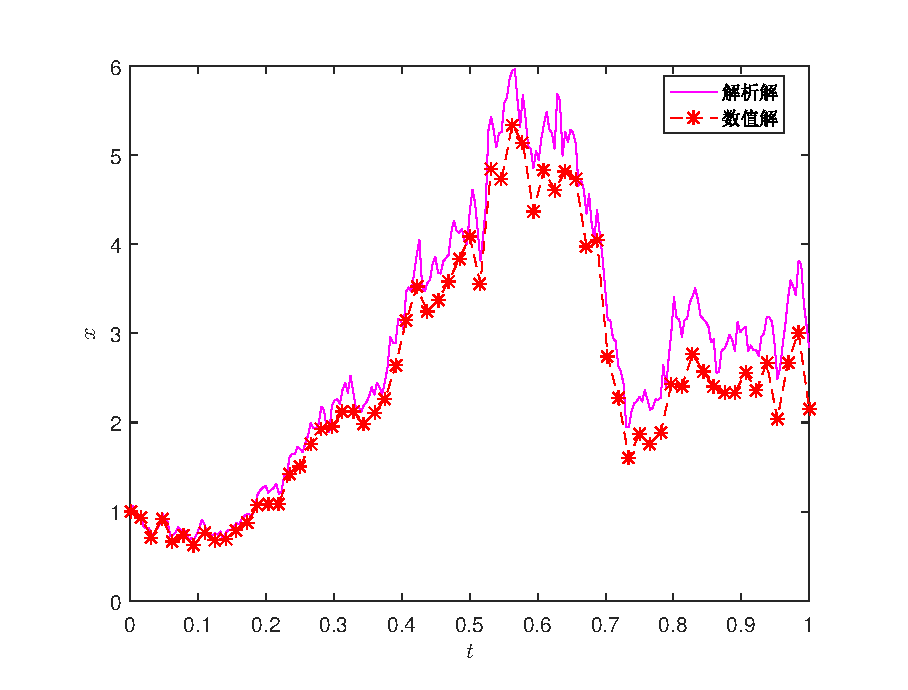
\includegraphics[width=8cm]{SDE_Euler.eps}
            \caption{SDE的Euler方法模拟图}
            \label{fig:SDE的Euler方法模拟图}
        \end{figure}
        % \textcolor[rgb]{1 0 0}{todo:matlab图片:sde-Euler方法}
    \subsection{解的收敛性与稳定性}
        \label{subsec:解的收敛性与稳定性}
        \subsubsection{收敛性}
            \label{subsubsec:收敛性}
            \par
            下面,我们来讨论一下数值解的收敛性。对某一点$t_n$而言,如果$X_{t_n}$与$X_n$并非随机变量,而是一个变量,我们自然希望$X_n$能够接近$X_{t_n}$,即估计量与真实值靠近(或者说数值解和解析解靠近)。但是在SDE中,估计量$X_n$和真实量$X_{t_n}$都是随机变量,这使得我们要重新找方法来衡量二者之间的接近度。
            \par
            假设我们可以重复计算$N$次SDE的解析解与数值解(注意,这里的$N$是对随机过程模拟$N$次),即对某一个$t_n$而言,进行$N$次采样$X_{t_n},X_n$,那么,就某时刻随机变量$X_n$和$X_{t_n}$的接近程度可以用
            \begin{align*}
            E[|X_n - X_{t_n}|]\approx \frac{1}{N} |X_n - X_{t_n}|
            \end{align*}
            来衡量(当然,也可以采用其它方法)。如果我们要求在每个时间点$t_n$上$E[|X_n - X_{t_n}|]$都非常小,那么就可以说数值解$X_n$是强收敛的。下面,给出SDE数值方法的收敛性和稳定性的概念。
            \begin{definition}[强收敛]
                在$[t_0,T]$上,令$h = \frac{T-t_0}{N}$,这个$N$为分割段数,$h$为步长。若$\exists c>0$,$c$与$h$无关,$\exists \delta > 0$,$h\in (0,\delta)$,使得$\forall t_n = t_0+nh\in [t_0,T]$,有
                \begin{align*}
                E[|X_n- X_{t_n}|] \leqslant ch^r
                \end{align*}
                其中:$X_{t_n}$为$t_n$时刻的解析解,$X_n$为$t_n$时刻的数值解。则称该数值方法是$r$阶强收敛的。
            \end{definition}

            \begin{definition}[局部收敛阶]
                若$\exists c>0$,$c$与$h$无关,令$\delta_n = X_n - X_{t_n}$
                为局部截断残差,有
                \begin{align*}
                \max_{0 \leqslant n \leqslant N}|E(\delta_n)| \leqslant ch^{p_1} \quad h\rightarrow 0
                \end{align*}
                以及
                \begin{align*}
                \max_{0 \leqslant n \leqslant N}\left(|E(\delta_n)^2| \right)^\frac{1}{2}\leqslant ch^{p_2} \quad h\rightarrow 0
                \end{align*}
                并且$p_1 \geqslant \frac 12,p_1 \geqslant p_2 + \frac 12$,则称$p_2$为该数值方法均方意义上的局部收敛阶。
            \end{definition}
            \begin{definition}[弱收敛]
                若对适当的$2(p+1)$次多项式$\varphi$,$\exists c>0,\delta >0,h\in (0,\delta)$,使得$\forall t_n = t0+nh\in [t_0,T]$,有
                \begin{align*}
                \Big|E[\varphi (X_n)] - E[\varphi(X(t_n))]\Big| \leqslant ch^p
                \end{align*}
                则称该数值方法为$p$阶弱收敛。
            \end{definition}
        \subsubsection{稳定性}
            \label{subsubsec:稳定性}
            \par
            关于解$X_t$的稳定性,可以参考ODE中的李雅普诺夫稳定。强(弱)收敛只是在有限时间$[t_0,T]$内讨论$X_t$的收敛效果,而当$t\rightarrow\infty$时,SDE的性质也是非常值得注意的。我们知道解$X_t$对初值是连续的,现在考虑初值微小波动对解的影响。
            \paragraph{平凡解稳定性}称$X(t;X_0,t_0) \equiv 0$是方程$\mathrm{d}X_t = f(X_t)\mathrm{d}t + g(X_t) \mathrm{d}W_t$的平凡解。1980年Has'mrnshiz给出了平凡解稳定性的定义:\\
            \ding{172}若$\forall \varepsilon >0,t_0>0$,有
            \begin{align*}
                \lim_{X_0\rightarrow 0}P\left(\sup_{t \geqslant t_0}|X(t;X_0,t_0| \geqslant \varepsilon \right) = 0
            \end{align*}
            则称$X(t;t_0,X_0)\equiv 0$是随机稳定的。\\
            \ding{173}若在随机稳定的前提下,有
            \begin{align*}
                \lim_{X_0\rightarrow 0}P\left(\lim_{t \rightarrow \infty}|X(t;X_0,t_0| \rightarrow 0 \right) = 1
            \end{align*}
            则称$X(t;t_0,X_0)\equiv 0$是随机渐进稳定的。\\
            \ding{174}若在随机渐进稳定的前提下,对$\forall X_0 \in R$,有
            \begin{align*}
                P\left(\lim_{t \rightarrow \infty}|X(t;X_0,t_0| \rightarrow 0 \right) = 1
            \end{align*}
            则称$X(t;t_0,X_0)\equiv 0$是大范围随机渐进稳定的。
            \paragraph{$p$阶矩稳定性}1992年,Kloeden和Dleten给出了$p$阶矩稳定的定义。若$\exists \varepsilon > 0,\exists \delta = \delta(\varepsilon,t_0)>0$,使得$\forall t \geqslant 0,|X_0|<\delta$,有
            \begin{align*}
            E\left( |X(t;X_0,t_0)|^p \right) < \varepsilon
            \end{align*}
            即$\exists \delta_0 = \delta(t_0)>0$,使得$\forall |X_0|<\delta$,有
            \begin{align*}
            \lim_{t\rightarrow \infty}E\left( |X(t;X_0,t_0)|^p \right) = 0
            \end{align*}
            则称$X(t;t_0,X_0) \equiv 0$是$p$阶矩渐进稳定的。特别地,当$p = 2$时,称为均方稳定(MS稳定)。
            \paragraph{MS稳定区域}
            对于任意一种数值方法,若迭代方程写为
            \begin{align}
                \label{一般形式的数值迭代方程}
                X_{n+1} = \phi(h,\lambda ,\mu ,J_n)X_n = \phi(h,\lambda,\mu,\sqrt{h}J)X_n
            \end{align}
            其中:
            \begin{align*}
                &J_n = W(t_{n+1}) - W(t_n) \sim N(0,h)\\
                &J\sim N(0,1)
            \end{align*}
            对上式(\ref{一般形式的数值迭代方程})两边取2阶原点矩,有
            \begin{align*}
                E \left( |X_{n+1}|^2 \right) = E \left( \phi^2 \right) + E \left( |X_n|^2 \right)
            \end{align*}
            我们称$R_1(h,\lambda,\mu) = E \left( \phi^2(h,\lambda,\mu,\sqrt{h}J) \right)$为均方稳定函数。若$|R_1(h,\lambda,\mu)|<1$,则该数值方法为均方稳定(MS稳定)。令$p = h\lambda,q = \sqrt{h}$,则迭代方程(\ref{一般形式的数值迭代方程})也可以写为
            \begin{align*}
            X_{n+1} = R_2(p,q)X_n
            \end{align*}
            称$R_2(p,q)$为均方稳定函数。若$|R_2(p,q)|<1$,则该数值方法MS稳定,并称$S = \{ (p,q)| |R_2(p,q)|<1\}$为该数值方法的MS稳定区域。
            \paragraph{T稳定}1993年,Saito和Mitsui提出T稳定。对于一般的数值迭代公式(\ref{一般形式的数值迭代方程})
            \begin{align*}
                X_{n+1} = \phi(h,\lambda ,\mu ,J_n)X_n = \phi(h,\lambda,\mu,\sqrt{h}J)X_n
            \end{align*}
            令
            \begin{align*}
                &\bar{X}_n = \sqrt[n]{\prod_{i = 1}^nX_i}\\
                &\bar{X}_{n+1} = \sqrt[n]{\prod_{i = 1}^nX_{i+1}}
            \end{align*}
            进一步得到一步差分方程
            \begin{align*}
                \bar{X}_{n+1} = R_T(h,\lambda,\mu)\bar{X}_n
            \end{align*}
            其中:
            \begin{align*}
                R_T(h,\lambda,\mu) = \sqrt[n]{\prod_{i=1}^n \phi(h,\lambda ,\mu ,J_i)}
            \end{align*}
            称$R_T(h,\lambda,\mu)$为T稳定函数。
    \subsection{数值方法}
        \label{subsec:数值方法}
        \par
        上面,我们利用Euler方法引出了数值解收敛性和稳定性的概念,下面再来介绍一些数值方法,并给出这些数值方法收敛性和稳定性的数值验证。考虑如下SDE问题
        \begin{align*}
            \mathrm{d}X_t = f(X_t) \mathrm{d}t + g(X_t)\mathrm{d}W_t
        \end{align*}
        \subsubsection{1.显示数值方法}
            \par
            1).显示Euler-Maruyama方法
            \begin{align*}
            X_{n+1} = X_n +f(X_n)\Delta t + g(X_n)\Delta W_n
            \end{align*}
            该方法是强0.5阶收敛,弱1阶收敛的。
            \par
            2).显示Milstein方法
            \begin{align*}
            X_{n+1} = X_n +f(X_n)\Delta t + g(X_n)\Delta W_n + \frac 12 g(X_n)g'(X_n)(\Delta W^2 - \Delta t)
            \end{align*}
            该方法是强1阶收敛的。
            \par
            3).显示R-K方法。Platen的一级显式R-K方法为
            \begin{align*}
            X_{n+1} &= X_n + f(X_n)\Delta t + g(X_n)\Delta W_n \\
            &\quad + \frac{1}{2\sqrt{\sigma}}\left[ g(X_n+ g(X_n)\sqrt{\sigma}) - g(X_n) \right](\Delta W^2 - \Delta t)
            \end{align*}
            其中:$\sigma$为$\Delta W_n \sim N(0,\sigma)$,例如$\sigma = \Delta t_n$。
            \par
            二级显式R-K方法
            \begin{align*}
                &X_{n+1} = X_n +\frac 34 K_1+ \frac 14 K_2 + \left( 1-\frac{f'(X_n)}{4} \Delta t \right)^{-2} g(X_n)\Delta W_n\\
                &K_1 = \left( 1-\frac{f'(X_n)}{4} \Delta t \right)^{-1}f(X_n)\Delta t\\
                &K_2 = \left( 1-\frac{f'(X_n)}{4} \Delta t \right)^{-1}f(X_n + K_1)\Delta t
            \end{align*}
            选取适当的参数,此方法可达到强1阶收敛。
            \par
            三级显式R-K方法
            \begin{align*}
                &X_{n+1} = X_n + \frac 16(K_1 +K_2 +K_3)+g(X_n)\Delta W_n\\
                &K_1 = f(X_n)\Delta t\\
                &K_2 = f(X_n+K_1)\Delta t\\
                &K_3 = f\left(X_n + \frac{K_1 +K_2}{4}\right)\Delta t
            \end{align*}
        \subsubsection{2.隐式数值方法}
            \label{subsubsec:2.隐式数值方法}
            \par
            1).隐式Euler-Maruyama方法
            \begin{align*}
            X_{n+1} = X_n + f(X_{n+1}) \Delta t+ g(X_{n+1})\Delta W_n
            \end{align*}
            该方法是强1阶收敛的。
            \par
            2).隐式Milstein方法
            \begin{align*}
            X_{n+1} &= X_n+f(X_{n+1})\Delta t + g(X_{n+1})\Delta W_n\\
             &\quad + g(X_{n+1})g'(X_{n+1})(\Delta W^2 - \Delta t)
            \end{align*}
            \par
            3).隐式R-K方法(二级)
            \begin{align*}
                &X_{n+1} = X_n +\frac 34 K_1+ \frac 14 K_2 + \left( 1-\frac{f'(X_{n+1})}{4} \Delta t \right)^{-2} g(X_{n+1})\Delta W_n\\
                &K_1 = \left( 1-\frac{f'(X_{n+1})}{4} \Delta t \right)^{-1}f(X_{n+1})\Delta t\\
                &K_2 = \left( 1-\frac{f'(X_{n+1})}{4} \Delta t \right)^{-1}f(X_{n+1} + K_1)\Delta t
            \end{align*}
            \par
            注意到,隐式数值方法中的$X_{n+1}$并不能直接计算,解决这个问题的一种可行的方法是:预估-矫正方法。例如,我们先用显式Euler-Maruyama方法预估$X_{n+1}$为
            $\tilde{X}_{n+1}$,然后再带入到隐式数值方法中进行计算。
            \begin{align*}
            \tilde{X}_{n+1} &= X_n+f(X_n)\Delta t +g(X_n)\Delta W_n\\
            X_{n+1} &= X_n+f(\tilde{X}_{n+1})\Delta t + g(\tilde{X}_{n+1})\Delta W_n\\
             & \quad + g(\tilde{X}_{n+1})g'(\tilde{X}_{n+1})(\Delta W^2 - \Delta t)
            \end{align*}
        \subsubsection{半隐式数值方法}
            \label{subsubsec:半隐式数值方法}
            \par
            以半隐式EM(Euler-Maruyama)方法为例,其余半隐式方法类推。半隐式EM方法为
            \begin{align*}
            X_{n+1} = X_n + (1-\theta )f(X_n)\Delta t+ \theta f(X_{n+1})\Delta t+ g(X_n)\Delta W_n
            \end{align*}
            其中:$\theta \in [0,1]$,半隐式方法的$f$是显式方法和隐式方法的结合,而扩散函数$g$是显式方法。特别地,当$\theta  = 0$时,为显示EM方法,当$\theta = 1$时,称为后退(back)EM方法,即
            \begin{align*}
            X_{n+1} = X_n + f(X_{n+1})\Delta t+ g(X_n)\Delta W_n
            \end{align*}
            注意:\\
            1.EM方法收敛于Ito型SDE而非Stratonovich型SDE;\\
            2.前面讨论的EM、Milstein和R-K方法都是一步数值方法,$X_{n+1}$的计算只需要$X_n$;\\
            3.前面讨论的数值方法都是在相应SDE下的。
        \subsubsection{双隐式数值方法}
            \label{subsubsec:双隐式数值方法}
            \par
            以双隐式Milstein方法为例,其余双隐式方法类推。双隐式Milstein方法为
            \begin{align*}
            X_{n+1} &= X_n + (1-\theta )f(X_n)\Delta t+ \theta f(X_{n+1})\Delta t+ g(X_n)\Delta W_n\\
            &\quad + L'g(X_n)\Delta W_n^2 - \frac{1- \sigma}{2} L'g(X_n)\Delta t -\frac{\sigma}{2}L'g(X_{n+1})\Delta t
            \end{align*}
            其中:$\theta \in [0,1]$,$\sigma \leqslant 1$ ,$L' = g\frac{\partial}{\partial x}$。
            \par
            双隐式Milstein方法是强1阶收敛的,其全局MS稳定的充要条件为
            \begin{align*}
            (2\lambda + \mu^2) + \Delta t\lambda^2(1-2\theta)+\frac{\Delta t \mu^2}{2}(2\sigma \lambda+ \mu^2)<0
            \end{align*}
            特别地,当$\theta = \sigma = 1$时,其MS稳定的充要条件为
            \begin{align*}
            (2\lambda + \mu^2) - \Delta t\lambda^2+\frac{\Delta t \mu^2}{2}(2 \lambda+ \mu^2)<0
            \end{align*}
%            \begin{figure}[H]
%            \centering
%            \includegraphics[width=7cm]{MS_stable_domain.eps}
%            \caption{MS稳定域图像}
%            \label{fig:MS稳定域图像}
%            \end{figure}
            % \textcolor[rgb]{1 0 0}{todo:matlab图片:MS稳定域图像}\\
    \subsection{数值实验}
        \label{subsec:数值实验}
        \par
        前面给出一类SDE在全局L(Lipschitz)条件及线性增长条件下的解的存在唯一性、SDE解析解数值解及解的收敛性和稳定性。下面,我们对数值方法的收敛性和稳定性进行数值验证。仍然考虑如下Black-Scholes方程(在Euler方法中我们用之进行了数值实验)
        \begin{align*}
            \left\{
            \begin{aligned}
            &\mathrm{d}X_t = \lambda X_t \mathrm{d}t + \mu X_t \mathrm{d}W_t\\
            &X(t_0) = X_0\\
            &t\in [t_0,T]
            \end{aligned}
            \right.
        \end{align*}
        上述SDE的解析解为
        \begin{align*}
            X_t = X_0\exp\left( \left( \lambda -\frac 12 \mu^2\right)t + \mu W_t \right)
        \end{align*}
        \par
        下面,我们分别对EM法、Milstein方法和R-K方法的收敛性和稳定性进行验证。仍采用之前的参数设置,令方程中的参数为:$\lambda = 2$,$\mu = 1$,$t_0 = 0$,$X_0 = 1$,$T = 1$,$N = 2^8$,$h = \Delta t = \frac{T - t_0}{N}$。
        \subsubsection{Euler方法的数值实验}
            \label{subsubsec:Euler方法的数值实验}
            \paragraph{Euler方法的强0.5阶收敛性验证}
            由强收敛性的定义我们知道,在任意时刻$t_n$上,$E(|X_n - X_{t_n}|)$都非常小,满足$E(|X_n - X_{t_n}|) \leqslant ch^\frac{1}{2}$。由于是任意时刻,这里不妨取末端时刻$T(T = Nh)$(当然可以取其他时刻),令
            \begin{align*}
            e_h = E(|X_n - X_{T}|)
            \end{align*}
            假设我们取定某个步长$h$,且进行$10000$次模拟,那么我们可以计算出该步长下的$e_h$。如果EM方法的强收敛阶为0.5,那么应该有
            \begin{align*}
            e_h \leqslant ch^\frac{1}{2}
            \end{align*}
            上式两边都是步长$h$的函数,两边同时取对数,有
            \begin{align*}
            \log e_h \approx \log c + \frac 12 \log h
            \end{align*}
            \par
            我们取不同的步长$h_1,h_2,h_3,\dots$。如果$\log e_h$和$\log h$所绘成的直线斜率接近$\frac 12$,则说明EM方法的强收敛阶确实为0.5。
            \par
            作为实验,这里,我们取步长$h_1 = 2^{-8},h_2 = 2^{-7},h_3 = 2^{-6},h_4 = 2^{-5},h_5 = 2^{-4}$,对每个步长$h_i$,在$[0,1]$上计算解析解与数值解10000次,然后计算$e_{h_i} = E(|X_n - X_T|) $,最终画$\log e_h$和$\log h$图,如图(\ref{fig:EM方法的强收敛阶验证})所示
           \begin{figure}[H]
           \centering
           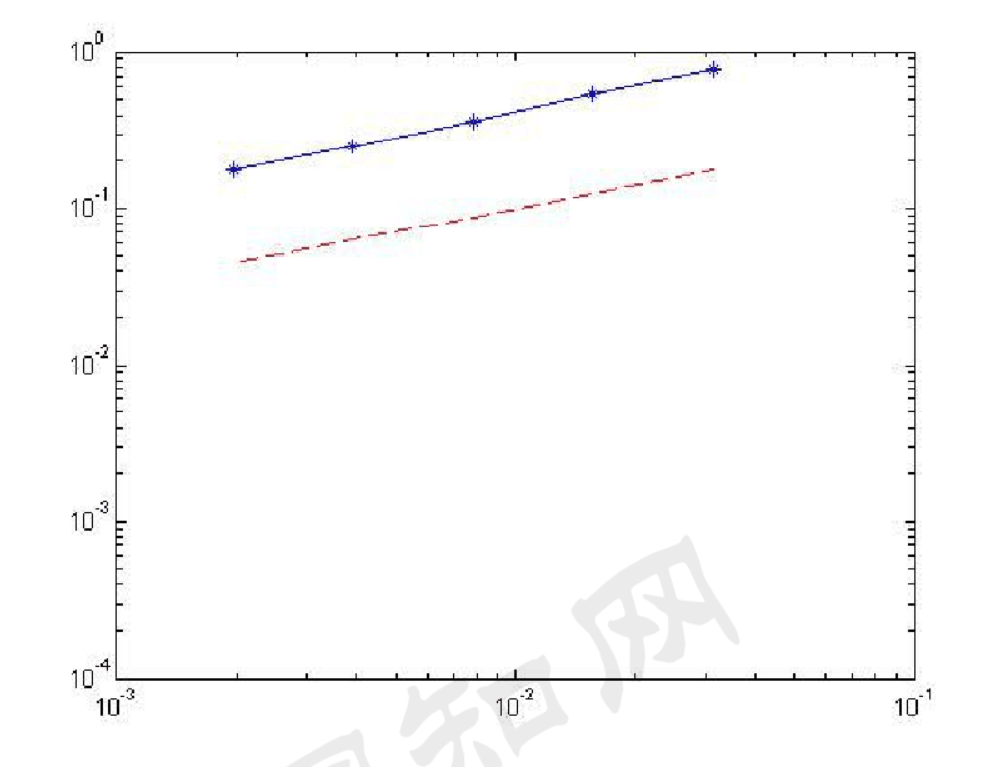
\includegraphics[width=7cm]{images/EM_Strong_convergence_prove.png}
           \caption{EM方法的强收敛阶验证}
           \label{fig:EM方法的强收敛阶验证}
           \end{figure}
            % \textcolor[rgb]{1 0 0}{todo:Matlab图片:EM方法的强收敛阶验证}

            \paragraph{Euler方法的稳定域的求取}
            在判定Euler方法的稳定性之前,我们先来求解Euler方法的稳定域。
            \par
            1).显式Euler方法的稳定域
            \begin{align*}
                X_{n+1} &= X_n + \lambda X_n h + \mu X_n \Delta W_n\\
                &=X_n + \lambda h + \mu X_n\sqrt{h}\xi\\
                &=(1+\lambda h +\mu \sqrt{h}\xi)X_n
            \end{align*}
            令$p = \lambda h,q = \mu \sqrt{h}$,有
            \begin{align*}
            X_{n+1} = (1 + p+ q\xi)X_n
            \end{align*}
            对上式两边求2阶原点矩,有
            \begin{align*}
                E(|X_{x+1}|^2) = E \left( (1+p+q\xi)^2X_n ^2\right)
            \end{align*}
            注意到$\xi \sim N(0,1)$,我们得到EM方法的MS稳定函数为
            \begin{align*}
                R_2 = (1+p)^2 +q^2
            \end{align*}
            当$R_2<1$时得到稳定域如图(\ref{fig:显式EM方法的稳定域示意图})所示
            \begin{lstlisting}[language = Matlab]
            h = ezplot('(1+p)^2+q^2-1',[-2,0],[0,1.5]);
            set(h, 'LineStyle','-','color', 'r')
            xlabel('p = lambda*h')
            ylabel('q = mu * sqrt(h)')
            \end{lstlisting}
           \begin{figure}[H]
           \centering
           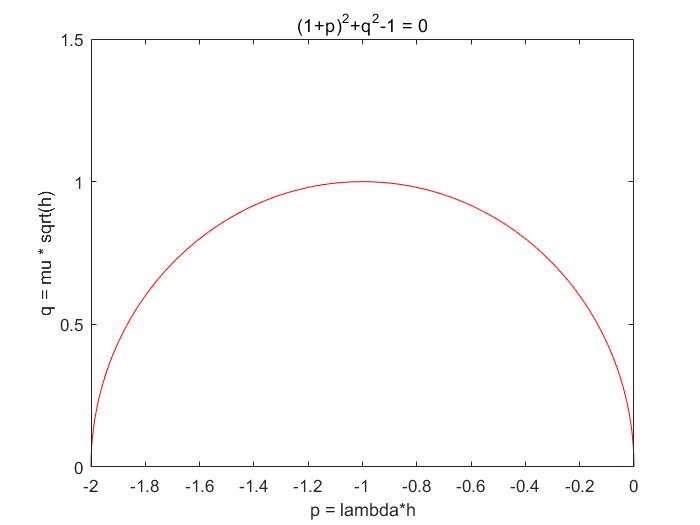
\includegraphics[width=7cm]{images/EM_stable_domain.jpg}
           \caption{显式EM方法的稳定域示意图}
           \label{fig:显式EM方法的稳定域示意图}
           \end{figure}
            % \textcolor[rgb]{1 0 0}{todo:Matlab图片:显式EM方法的稳定域示意图}
            \par
            2).半隐式EM方法的稳定域。迭代公式为
            \begin{align*}
            X_{n+1}=\frac{1+q\xi}{1-p}X_n
            \end{align*}
            其均方稳定函数为
            \begin{align*}
            R_2 = \frac{1+q^2}{(1-p)^2}
            \end{align*}
            \par
            3).隐式EM方法的稳定域。其迭代公式为
            \begin{align*}
            X_{n+1} = \frac{1}{1-p-q\xi + q^2 \xi^2} X_n
            \end{align*}
            其均方稳定函数为
            \begin{align*}
            R_2 = \frac{1}{\sqrt{2\pi}}\int_{- \infty}^{\infty}\frac{1}{( ( qx - \frac 12 )^2 +\frac {3}{4} - p )^2 } e^{-\frac{x^2}{2}}\mathrm{d}x
            \end{align*}

            \paragraph{Euler方法的稳定性验证}
            取不同步长$h_1 = 1,h_2 = \frac 12,h_3 = \frac 14$,在$[0,20]$区间上进行观察,对每个步长$h_i$,用Euler方法迭代10000次,求取均值$E(|X_t|^2)$,并进行绘图,如图(Euler方法稳定性验证图)
           \begin{figure}[H]
           \centering
           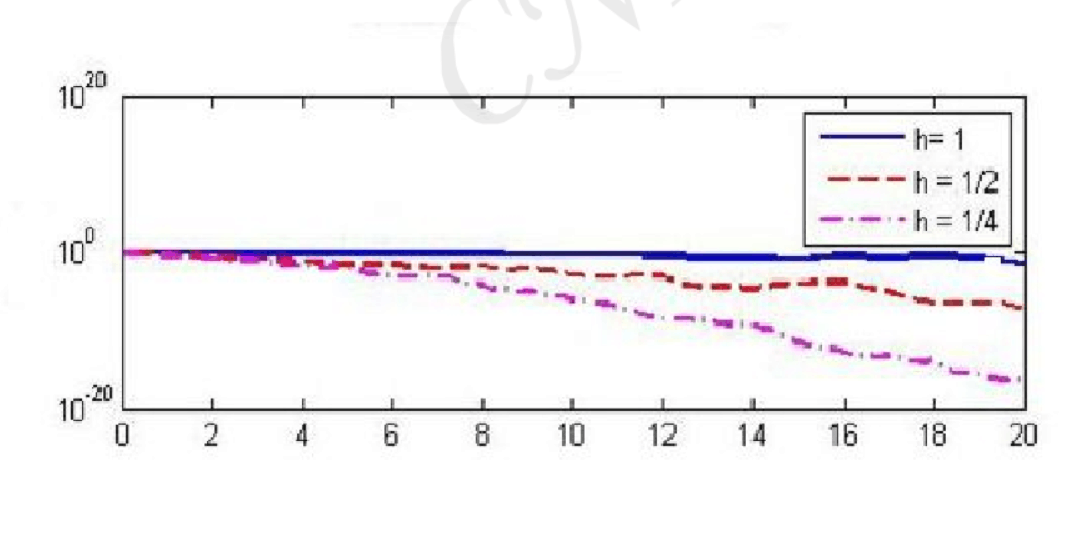
\includegraphics[width=8cm]{images/Euler_stable.png}
           \caption{Euler方法稳定性验证图}
           \label{fig:Euler方法稳定性验证图}
           \end{figure}
            % \textcolor[rgb]{1 0 0}{todo:Matlab图片:Euler方法稳定性验证图}\\
            观察上图中当$t\rightarrow \infty$时$\lim\limits_{t\rightarrow \infty}E(|X_t|^2)$
            的性质,如果$\lim\limits_{t\rightarrow \infty}E(|X_t|^2) = 0$,说明EM方法MS稳定,并且发现$p,q$在稳定域中。
        \subsubsection{Milstein方法的数值实验}
            \label{subsubsec:Milstein方法的数值实验}
            \paragraph{Milstein方法的稳定域的求取}
            Milstein方法的强1阶收敛性的验证和稳定性检验可以参考Euler方法。下面,我们主要介绍Milstein方法的稳定域的求解。
            \par
            1.显式Milstein方法的迭代公式为
            \begin{align*}
            X_{n+1} = (1+p+q\xi+q^2(\xi^2 - 1)/2)X_n
            \end{align*}
            其均方稳定函数为
            \begin{align*}
            R_2(1+p)^2 + q^2 + \frac 12 q^4
            \end{align*}
            \par
            2.半隐式Milstein方法的均方稳定函数为
            \begin{align*}
            R_2 = \frac{2(1+(1-\theta)p)^2 + 2q^2 + q^4}{2(1-\theta p)}
            \end{align*}
            \par
            3.隐式Milstein方法的均方稳定函数为
            \begin{align*}
            R_2 = \frac{1}{\sqrt{2 \pi}}\int_{-\infty}^{\infty} \frac{4}{(3-2p+q^2-(qx-1)^2)^2}e^{\frac{x^2}{2}}\mathrm{d}x
            \end{align*}

        \subsubsection{R-K方法的数值实验}
            \label{subsubsec:R-K方法的数值实验}
            上面提到的EM方法和Milstein方法是收敛于Ito型SDE,而对Stratonovich型SDE而言,R-K方法是较高效的。
            \paragraph{R-K方法的稳定域的求取}R-K方法的强1阶收敛性的验证和稳定性检验可以参考Euler方法。下面,我们主要介绍R-K方法的稳定域的求解。
            \par
            1.显式2级R-K方法的迭代公式为
            \begin{align*}
            X_{n+1} = X_n \left[ 1+\frac{(2\lambda h- \mu ^2h + 2\mu \sqrt{h}\xi)(4+2\lambda h-\mu ^2h+2\mu\sqrt{h}\xi)}{8}  \right]
            \end{align*}
            令$p = \lambda h,q = \sqrt{h}\mu,\xi \sim N(0,1)$,有MS稳定函数为
            \begin{align*}
            R_2 &= \frac{1}{64}[64+16(2p-q^2)(2p-q^2+4)+64q^2\\
            &\quad+(2p-q^2)^2(2p-q^2+4)^2+4q^2(2p-q^2)^2\\
            &\quad+4q^2(2p-q^2+4)^2+48q^4+16q^2(2p-q^2)(2p-q^2+4)]
            \end{align*}
            \par
            2.半隐式2级R-K方法的迭代公式为
            \begin{align*}
            X_{n+1} = X_n\left[  1+ \frac{(2\lambda h - \mu^2h+2\mu\sqrt{h}\xi)(2-6\lambda h +3\mu^2 h+4\mu\sqrt{h}\xi)}{4(2-2\lambda h +\mu^2h)^2}\right]
            \end{align*}
            其MS稳定函数为
            \begin{align*}
            R_2 &= 1+\frac{4p-12p^2+12pq^2+6q^2-3q^4}{2(2-2p+q^2)^2}\\
            &\quad + \frac{(2p-q^2)^2(2-6p+3q)^2+16q^2(2p-q^2)^2+192q^4}{16(2-2p+q^2)^4}\\
            &\quad +\frac{32q^2(2p-q^2)(2-6p+3q^2)+4q^2(2-6p+3q^2)^2}{16(2-2p+q^2)^4}
            \end{align*}
            \par
            3.隐式2级R-K方法的迭代公式为
            \begin{align*}
            X_{n+1} = X_n\left[ 1+\frac{(2\lambda h-\mu^2h+2\mu\sqrt{h}\xi)(4-6\lambdah+3\mu^2h-6\mu\sqrt{h}\xi)}{2(2-2\lambda h+\mu^2h-2\mu\sqrt{h}\xi)^2} \right]
            \end{align*}
            其MS稳定函数为
            \begin{align*}
            R_2 = \frac{1}{\sqrt{2\pi}}\int_{-\infty}^{\infty}\left[ 1+\frac{(2p-q^2+2qx)(4-6p+3q^2-6qx)}{2(2-2p+q^2 - 2qx)^2} \right]e^{-\frac{x^2}{2}}\mathrm{d}x
            \end{align*}
            \par
            1.对于上面介绍的数值方法的收敛性和稳定性,我们是直接给出其收敛阶和稳定性,然后再用数值方法进行验证。那么,如何依据收敛性和稳定性的定义来证明某些数值方法的收敛性和稳定性呢?2.可以看到,解析解$X_{t_n}$与数值解$X_n$都是随机过程,所以对于解析解和数值解都会有收敛性和稳定性。
        \subsubsection{注记}
            1992.Kloedn和Platen在文献\cite{1992.Kloeden}中通过随机泰勒展开方法得到了一系列数值方法。1995.Milstein在文献\cite{1995.Milstein}中研究了泰勒展开及随机R-K方法的弱收敛性和均方强收敛性。2004.Milstein和Tretyakov在文献\cite{2004.Milstein}中进一步研究了R-K方法的MS稳定性。2005.Rodkina研究了半隐式变步长$\theta$方法的几乎渐近稳定性。2006.Buchwar和Winkler研究了一类随机线性多步方法。同年,利用Lypronov函数研究了两步Maruyama方法的均方渐进稳定性。2007.Kossler基于彩色根树理论研究了R-K方法的2阶弱收敛性。2008Kim和Stanescu给出了低存储高效率的1.5阶R-K方法。2008.Sickenberger研究了变步长多步方法的均方收敛性。2010.Debrabant研究了3阶弱收敛的R-K方法。

\section{SDE解存在唯一条件的进一步讨论}
    \par
    考虑如下问题:CEV(Constarit Elastictiy of Variance Model)
    \begin{align*}
        \left\{
            \begin{aligned}
            &\mathrm{d}X_t = \mu X_t + \sigma X_t^r \mathrm{d}W_t\\
            &X(t_0) = X_0
            \end{aligned}
        \right.
    \end{align*}
    上面的CEV模型中,当$r=1$时,模型是我们前面所讨论的SDE模型;当$0<r<1$时,模型中的漂移项$\sigma X_t^r$显然不满足全局$L$条件。我们说SDE在全局L条件和线性增长条件下存在唯一解,那么,如果$f,g$不满足全局L条件或者线性增长条件,我们应该怎样解决?后面我们将尝试着解决如下的问题:
    \par
    (1)在模型结构不变的情况下,即SDE的形式仍为
    \begin{align*}
        \mathrm{d}X_t = f(X_t)\mathrm{d}t + g(X_t)\mathrm{d}W_t
    \end{align*}
    若$f,g$不满足全局L条件和线性增长条件,SDE的解存在唯一吗?解析解和数值解如何求取?解的收敛性和稳定性如何?
    \par
    (2)如果模型形状改变,如引入Poisson跳、Markov切换、延迟项和分数阶等等,那么模型的性质如何?
    \par
    针对问题(1),我们给出$f,g$在其它条件下(如局部L条件和Khasminskii条件)解的存在唯一性,并介绍EM方法、双隐Milstein方法、(半)驯服方法和分裂步等方法用于数值计算。
    \subsection{非全局Lipschitz条件下解的存在唯一性}
        \label{subsec:非全局Lipschitz条件下解的存在唯一性}
        \par
        1975年,Fridman在文\cite{1975.Fridman}中研究了局部L条件想和线性增长条件下的解的存在唯一性。1980年,Khasminskii在文\cite{1980.Khasminskii}中研究了在不满足线性增长条件而是满足Khasminskii条件下,解的存在性,并给出Euler方法的依概率收敛性。
        \subsubsection{非全局L条件}
            \label{subsubsec:非全局L条件}
            \par
            下面,我们来介绍一些非局部L条件。考虑如下SDE模型
            \begin{align*}
                \left\{
                    \begin{aligned}
                    &\mathrm{d}X_t = f(X_t ) + g(X_t) \mathrm{d}W_t\\
                    &X(t_0) = X_0\\
                    &t\in [t_0,T]
                    \end{aligned}
                \right.
            \end{align*}
            其中:$X_0\in R$,$W_t$是一维Brown运动(可以将Brown运动扩展到高维)。
            \par
            1).全局L条件。
            如果$f\in C^1(R)$且$\exists L >0$,使得$\forall x,y \in R$,有
            \begin{align*}
                |f(x) - f(y)  | \leqslant L|x-y|
            \end{align*}
            则称函数$f$满足全局L条件。
            \par
            2).单边L条件。
            如果$f \in C^1$,且$\exists L>0$,使得$\forall x,y\in R$,有
            \begin{align*}
                \bigl<x-y,f(x) - f(y)\bigr> \leqslant L|x-y|^2
            \end{align*}
            则称$f$满足单边L条件。
            \par
            3).局部L条件。
            如果$f\in C^1$,对每个常数$j$,$\exists L_j >0$,使得$\forall x,y \in R,|x|\vee |y|<j$,有
            \begin{align*}
                |f(x) - f(y) | \leqslant L_j |x-y|
            \end{align*}
            则称$f$满足局部L条件。其中:$|x|\vee |y| = \max\{x,y\} $ 。
            \par
            4).线性增长条件。
            如果$f\in C^1$,并且$\exists L>0$,使得$\forall x\in R$,有
            \begin{align*}
                |f(x)|^2 \leqslant L(1+|x|^2)
            \end{align*}
            则称$f$满足线性增长条件。
            \par
            5).Khasminskii型条件。
            $\forall (x,y)\in R^n\times R^n$,$\exists v\in C^2(R^n;R^+),\alpha > 0$,使得
            \begin{align*}
            \lim_{|x|\rightarrow \infty} \inf v(x) = \infty
            \end{align*}
            和
            \begin{align*}
                Lv(x,y) \leqslant \alpha (1+v(x)+ v(y))
            \end{align*}
            其中:$Lv:R^d\times R^d \rightarrow R$。若$v\in C^{2,1}(R^d;R)$,则$Lv$定义为
            \begin{align*}
                Lv(x,y,t) = v_t(x,t) + v_x(x,t)f(x,y) + \frac 12\mathrm{trac}\left[g^{\mathrm{T}}(x,y)v_{xx}(x,t)g(x,y)\right]
            \end{align*}

        \subsubsection{解的存在唯一性}
            \par
            上面介绍了一些非全局L条件,下面我们给出在这个非全局L条件下,SDE解的存在唯一性。
            \paragraph{单边L条件下的存在唯一性}
            如果$f,g\in C^1(R)$,且$f$满足常数$\mu$的单边L条件,$g$满足常数$\bar{C}$的全局L条件,即$\exists \mu, \bar{C}>0$,使得$\forall x,y \in R$,有
            \begin{align*}
            &\bigl<x-y,f(x)-f(y)\bigr> \leqslant \mu |x-y|^2\\
            &|g(x)- g(y) |^2 \leqslant \bar{C}|x-y|^2
            \end{align*}
            则SDE存在唯一解,并且有对$\forall p \geqslant 2$,$\exists C = C(p,T)>0$,使得
            \begin{align*}
            E \left[ \sup_{0 \leqslant t \leqslant T} |X_t|^p\right] \leqslant C(1+E|X_0|^p)
            \end{align*}
            注:上面仅仅是解存在唯一的充分条件,而非必要。
            \paragraph{局部L条件下的存在唯一性}如果$f,g\in C^1(R)$,并且$f,g$满足局部L条件,即对每个正整数$j$,$\exists K_j$,使得$\forall x,y \in R,|x|\vee |y|<j$,有
            \begin{align*}
                |f(x) - f(y) | \leqslant K_j |x-y|
            \end{align*}
            则SDE存在唯一局部解。在此基础上,如果$\exists \gamma >0$,使得$\forall x,y\in R$,有
            \begin{align*}
                2xf(x)+|g(x)|^2 < -\gamma|x|^2
            \end{align*}
            则SDE存在唯一全局解,并且$X_t$指数均方稳定
            \begin{align*}
            E|X_t|^2 \leqslant C(X_0) e^{-\gamma t}
            \end{align*}
            其中:$C(X_0)$是一个依赖于初始值$X_0$的常数。
            \par
            值得一提的是,当$f$满足单边L,$g$满足全局L时,可以由均值定理得到$f,g$满足局部L,另外
            \begin{align*}
            \bigl<x,f(x)\bigr> \vee |g(x)|^2 \leqslant\alpha + \beta|x|^2
            \end{align*}
            其中:$\alpha = \frac 12 |f(0)|^2 \vee 2|g(0)|^2$,$\beta = (\mu+\frac 12)\vee 2\bar{C}$。更多的内容可以参考1997.Mao\cite{1997.Mao}。
    \subsection{非全局Lipschitz条件下数值方法}
        \par
        上面,我们给出了SDE在某些条件下解的存在唯一性,下面,我们将要讨论某些数值方法的收敛性和稳定性。
        \paragraph{Euler方法}
        以Euler方法为例,2002年Higham, Mao和Stuor\cite{2002.Higham}给出在$f,g$满足局部L条件,或者$f$满足单边L条件,$g$满足全局L条件下,当单边L条件常数$c$、Euler方法中的$\theta$和步长$\Delta = h$满足$c\theta\Delta <1$以及SDE解析解和数值解矩有界条件下,Euler方法是强收敛的,即对$\forall p>2$,有
        \begin{align*}
            E \left[ \sup_{0 \leqslant n \leqslant N}|X_n|^p \right] < \infty\\
            E \left[ \sup_{0 \leqslant n \leqslant N}|X_{t_n}|^p \right] < \infty
        \end{align*}
        则
        \begin{align*}
            \lim_{\Delta t \rightarrow 0}E\left[\sup_{0 \leqslant n \leqslant N}|X_n - X_{t_n}|^2 \right] = 0
        \end{align*}
        Mao和Szpvuch在《Strong Convergance rates for back ward》还证明了在单边L条件结合一类多项式增长条件结合多项式L条件下,BackEuler方法的强收敛阶为0.5。
        \par
        现在,我们介绍具体的Euler方法。考虑如下两类Euler方法\\
        1).$\theta$-Euler方法
        \begin{align*}
        X_{n+1} = X_n + \theta f(X_{n+1})\Delta t + (1-\theta)f(X_n)\Delta t+ g(X_n)\Delta W_n
        \end{align*}
        2).分裂步-Euler方法
        \begin{align*}
            \left\{
                \begin{aligned}
                &X_n = y_n + \theta f(X_n)\Delta t\\
                &y_{n+1} = y_n +f(X_n)\Delta t+g(X_n)\Delta W_n\quad n = 0,1,\dots,N-1
                \end{aligned}
            \right.
        \end{align*}
        其中:$X_0 = X(t_0)$,$t_0 = 0$,$\theta\in [0,1]$。
        \par
        对于上述Euler方法,我们关心两个问题:1.收敛性2.稳定性。对于上述两种Euler方法的收敛性,我们有如下结论:
        \begin{theorem}[Euler方法的收敛性]
        在SDE存在唯一解的情况下,当$\theta\in [0,\frac 12 )$且$f$满足线性增长条件时,或者当$\theta\in (\frac 12 ,1]$时,对$\forall p \geqslant 2$,$\forall t_n\in[0,T]$,有
        \begin{align*}
        &\lim_{\Delta t \rightarrow 0}E\left[\sup_{t_n \in[0,T]}|X_n - X(t_n)|^p \right] = 0\\
        &\lim_{\Delta t \rightarrow 0}E\left[\sup_{t_n \in[0,T]}|X_n - y(t_n)|^2 \right] = 0
        \end{align*}
        \end{theorem}
        \par
        但上述结论并没有给出Euler方法的收敛阶数,对于两类Euler方法的强0.5阶收敛性,我们有如下结论:
        \begin{theorem}[强0.5阶收敛性]
        在SDE存在唯一解的情况下,若$\exists D,q>0$,使得$\forall x\in R$,有
        \begin{align*}
        |f'(x)| \leqslant D(1+|x|^q)
        \end{align*}
        且对$\Delta t < \underline{\Delta}$,$\theta\in[0,1]$,当$\theta \in [0,\frac 12)$时,$f$满足线性增长条件,则$\forall p \geqslant 2$,有
        \begin{align*}
        E\left[\sup_{t_n \in[0,T]}|X_n - X(t_n)|^p \right] \leqslant C(\Delta t)^{\frac p2}\\
        E\left[\sup_{t_n \in[0,T]}|X_n - y(t_n)|^p \right] \leqslant C(\Delta t)^{\frac p2}
        \end{align*}
        其中:$\Delta t = h$,$\forall t_n\in [0,T]$
        \begin{align*}
            \underline{\Delta} =
            \left\{
                \begin{aligned}
                &\infty ,&\theta  = 0\\
                &\frac{1}{2\theta\beta },&\theta > 0
                \end{aligned}
            \right.
        \end{align*}
        \end{theorem}
        上述结论证明可参考\cite{zong.2014}宗小峰.华中科技大学博士论文《随机微分方程的数值分析及随机稳定化》。
        \par
        上面给出了Euler方法的收敛性,下面讨论Euler方法的稳定性。在SDE精确解存在唯一且指数均方稳定条件下,我们来研究Euler数值方法的稳定性,并且为了保证Euler方法在$\theta\in(0,1]$时有意义,我们假设$f$满足单边L条件。
        \begin{theorem}[Euler稳定性]
        如果$f,g$满足局部L条件,且$\exists \gamma >0$,使得$\forall x,y\in R$,有
        \begin{align*}
            2xf(x)+|g(x)|^2 \leqslant -\gamma |x|^2
        \end{align*}
        则SDE存在唯一全局解,并且满足
        \begin{align*}
        E|X_t| \leqslant C(X_0)e^{-\gamma t}
        \end{align*}
        \par
        在此情况下,如果$\theta \in [0,1]$且在$\theta\in (0,1]$时,$f$满足单边L条件,\\
        \ding{172}在$\theta \in [0,\frac 12]$时,$f$满足常数$K$的线性增长条件,则$\forall \Delta t< \Delta ^* :=\frac{\gamma}{(1-2\theta)K} \wedge\overline{\Delta} $,有
        \begin{align*}
        E|y_t|^2 \leqslant C(X_0)e^{-\gamma_{\Delta}K\Delta t}\\
        E|X_t|^2 \leqslant C(X_0)e^{-\gamma_{\Delta}K\Delta t}
        \end{align*}
        其中:
        \begin{align*}
        \gamma_{\Delta} = -\frac{1}{\Delta t}\log \left( 1-\frac{\gamma-(1-2\theta)\Delta tK}{(\theta\Delta t\sqrt{K}+1)^2} \Delta t\right)
        \end{align*}
        \ding{173}在$\theta \in [\frac 12,1]$时,对$\forall \Delta t < \overline{\Delta}$,有
        \begin{align*}
        E|y_t|^2 \leqslant C(X_0)e^{-\gamma_{\Delta}K\Delta t}\\
        E|X_t|^2 \leqslant C(X_0)e^{-\gamma_{\Delta}K\Delta t}
        \end{align*}
        其中:
        \begin{align*}
        \gamma_\Delta = -\frac{1}{\Delta t}\log \left( 1- \frac{\gamma(2\theta-1)}{2\theta -1+\gamma \Delta t\theta^2} \Delta t\right)
        \end{align*}
        \end{theorem}
        \par
        上述定理中的$\overline{\Delta }$为
        \begin{align*}
            \overline{\Delta } =
            \left\{
            \begin{aligned}
            &\frac{1}{\mu \theta},&\theta \in (0,1]\text{且}\mu>0\\
            &\infty ,&\theta = 0\text{或}\mu<0
            \end{aligned}
            \right.
        \end{align*}
        在$\theta \in [0,\frac 12]$时,经常需要$f$满足单边L条件的同时,还满足$\mu<0$,而在$\theta \in [\frac 12 ,1]$时,Euler方法是无条件保持稳定的;在$\theta \in [0,\frac 12]$时,在$f$满足线性增长条件下,两类Euler方法稳定,而在$\theta \in[\frac 12,1]$时,则不需要$f$的线性增长条件。
        \paragraph{Milstein方法}考虑如下两种Milstein数值方法
        \par
        1.$\theta$-Milstein方法
        \begin{align*}
        X_{n+1} = X_n + f(X_n)\Delta t+ g(X_n)\Delta W_t + \frac{ 1}{2}L'g(X_n)(|\Delta W_n|^2 - \Delta t)
        \end{align*}
        其中:$\Delta t= h$为步长,$L' = g(x)\frac{\partial}{\partial x}$。
        \par
        2.分裂步Milstein方法
        \begin{align*}
            \left\{
                \begin{aligned}
                &X_n = y_n + \theta f(X_n)\Delta t\\
                &y_{n+1} = y_n + f(X_n)\Delta t+ g(X_n)\Delta W_n + \frac{1}{2}L'g(X_n)(|\Delta W_n|^2 - \Delta t)\\
                &k = 0,1,\dots,N-1\\
                &y_0 = X(0)
                \end{aligned}
            \right.
        \end{align*}
        \par
        2013年,Higham等在文献\cite{2013.Higham}中提出双隐Milstein方法
        \begin{align*}
            X_{n+1} &= X_n+[(1-\theta)f(X_n) + \theta f(X_{n+1}) ]\Delta t + g(X_n)\Delta W_n\\
            &\quad +\frac 12 L'g(X_n)(\Delta W_n)^2 - \frac{1- \bar{\theta}}{2}L'g(X_n)\Delta t - \frac{\bar{\theta}}{2}L'g(X_{n+1})\Delta t
        \end{align*}
        并证明在单边L条件和单调条件下,该数值方法是强收敛的。其中:$\theta \geqslant 0,\bar{\theta} \leqslant 1,L' = g(x)\frac{\partial}{\partial x}$。
        \paragraph{驯服方法}2012年,Hutzentler在文\cite{2012.Hutzenthaler}中提出驯服(Tamed)-Euler方法
        \begin{align*}
            X_{n+1} = X_n + \frac{f(X_n)\Delta t}{1+|f(X_n)|\Delta t} + g(X_n)\Delta W_n
        \end{align*}
        并证明taned-Euler方法是标准0.5阶收敛的。2013年,Wang和Gan在文\cite{2013.Wang}中提出taned-Milstein方法
        \begin{align*}
        X_{n+1} = X_n +\frac{f(X_n)\Delta t}{1+|f(X_n)|\Delta t} + g(X_n)\Delta W_n + \frac{1}{2}L'g(X_n)(|\Delta W_n|^2 - \Delta t)
        \end{align*}
        并证明该方法是强1阶收敛的。
\section{SDE结构的进一步讨论}
    \par
    前面讨论的SDE模型的结构都是
    \begin{align*}
    \mathrm{d}X_t = f(X_t)\mathrm{d}t + g(X_t)\mathrm{d}W_t
    \end{align*}
    无论$f,g$是什么类型的函数,也不论$f,g$满足什么样的条件,SDE的结构都是上面的结构。下面,对SDE的结构进行如下的扩展:
    \begin{enumerate}
        \item SDE基本理论
        \item 含Markov切换的SDE
        \item 含Poisson跳的SDE
        \item 随机延迟微分方程SDDE
        \item 中立型SDE
        \item 分段连续SDE
        \item SDE参数估计问题
        \item 随机偏微分方程SPDE
        \item *随机控制
        \item *分数阶SDE
    \end{enumerate}
    \subsection{SDE基本理论}
        \par
        一般形式的SDE
        \begin{align*}
        \mathrm{d}X_t = b(t,X_t)\mathrm{d}t+\sigma(t,X_t)\mathrm{d}W_t
        \end{align*}
        其中:$X\in R^n$,$b:[0,T]\times R^n \rightarrow R^n$,$\sigma:[0,T]\times R^n \rightarrow R^{n\times d}$,$W_t$是$d$为Brown运动。
        \par
        上述SDE可以用于描述液体中由分子无规则碰撞的小颗粒的运动,因此,亦称SDE的解$X_t$为Ito分布。下面,我们来看一下时齐Ito分布的Markov性,时齐Ito分布是如下SDE的唯一解
        \begin{align*}
        \left\{
            \begin{aligned}
            &\mathrm{d}X_t = b(X_t)\mathrm{d}t+\sigma (X_t)\mathrm{d}W_t\\
            &X_s = x\\
            &t \geqslant s
            \end{aligned}
        \right.
        \end{align*}
        由于上述SDE有$X_s= x$的初始条件,所以将其解记为$X_t = X_t^{s,x}(t \geqslant s)$,若初始时刻$s = 0$,则记为$X_t = X_t^{0,x}$。\\
        注:在后面的BSDE部分,我们用$X_t^{t,x}(t \leqslant s \leqslant T)$表示初始时刻为$t$,初始条件为$X_t = x$的随机过程。
        \par
        引进$\{X_t\}_{t \geqslant 0}$的概率分布$Q^x(x\in R^n,X_0 = x)$,且令$\mathcal{F}_t$是Brown运动$W_t$产生的$\sigma$代数,$\mathcal{M}_t$是$X_t$产生的$\sigma$代数。由于$X_t$关于$\mathcal{F}_t$可测,所以$\mathcal{M}_t \subseteq \mathcal{F}_t$。下面,给出$X_t$的Markov性。
        \begin{theorem}[Ito分布的Markov性]
        设$f$为$R^n \rightarrow R$的Borel函数,则对$\forall t$,对$h \geqslant 0$,有
        \begin{align*}
        E^x\left[f(X_{t+h})|\mathcal{F}_t\right] = E^{X_t(w)}[f(X_h)]
        \end{align*}
        即$X_t$在$t$时刻后的行为与$X_t$在$t$时刻前的行为一样。
        \end{theorem}
        注:$X_t$的Markov性质是在$X_t$时齐性基础上得到的。$X_t$时齐性:$\{X_{s+h}^{s,x}\}_{h \geqslant 0 }$和 $\{X_{h}^{0,x}\}_{h \geqslant 0 }$ 具有相同分布。
        \par
        上面给出了$X_t$的Markov性,下面我们来介绍$X_t$的强Markov性。首先,给出停时$\tau$的定义
        \begin{definition}[停时]
            以$\{N_t\}$表示一个单增的$\sigma$代数族。如果$\forall t \geqslant 0$,有
            \begin{align*}
                \{w|\tau(w) \leqslant t\} \in N_t
            \end{align*}
            其中:$\tau:\Omega \rightarrow [0,\infty)$是一个随机函数。则称函数$\tau$为关于$\{N_t\}$的停时。
        \end{definition}
        \par
        停时的示例(首达时):$\{X_n\}$是一个随机变量序列,$A$是一个事件集,令
        \begin{align*}
            T(A) = \inf\{n|X_n\in A\}
        \end{align*}
        并且约定$T(1) = \inf\{n|X_n \in \varPhi \} = \infty$。可见$T(A)$是$\{X_n\}$首次进入$A$(即发生$A$中所包含事件)的时刻,称$T(A)$是$\{X_n\}$到集合$A$的首达时。可证明$T(A)$是关于$\{X_n\}$的停时。
        \begin{theorem}[Ito分布的强Markov性]
            已知$f$是$R^n$上的Borel函数,$\tau$是关于$\mathcal{F}_t$的停时,$\tau < \infty,a.s$,则
            \begin{align*}
            E^x\left[f(X_{\tau+h})|\mathcal{F}_t\right] = E^{X_{\tau}}[f(X_h)]\quad h \geqslant0
            \end{align*}
            粗略来讲,强Markov性就是将Markov性中的$t$变为停时$\tau$。
        \end{theorem}
        \begin{theorem}[Dynkin公式]
            已知$f\in C_0^2(R^n)$。设$\tau$是一个停时,$E^x(\tau) < \infty$,则
            \begin{align*}
            E^x[f(X_{\tau})] = f(x) + E^x\left[\int_0^{\tau}Af(x_s)\mathrm{d}s\right]
            \end{align*}
        \end{theorem}
        \textcolor[rgb]{1 0 0}{todo:未完待续。}

    \subsection{含Markov切换的SDE}
        \par
        1961年,Karsovskii和Lidslcii第一次在线性模型中引入切换,形成线性切换模型。他们在模型中使用连续马尔科夫链来描述这种不同模型结构之间的切换。我们将这种Markov切换的思想引入到SDE模型当中,带Markov切换的SDE的状态空间分为离散状态和连续状态,用Markov链来模拟离散状态,用SDE来模拟连续状态。并且由于不同过程之间相互干扰,这使得随机系统变得更加难于处理。大量的实验表明:Brown运动、Markov切换和Poisson过程等随机因素的引入可以使一个不平稳的系统稳定化(当然,反之亦可),这个观点被称为随机稳定化。下面,我们将简单介绍一下带Markov切换的SDE,以及其随机稳定化。
        \par
        令$r(t) \equiv r_t$为取之于有限空间$S = \{1,2,\dots,N\}$的右连续Markov链,并且有生成元(状态转移矩阵)$\Gamma = (r_{ij})_{N \times N}$,其转移概率为
        \begin{align*}
            p(r(t+\delta) =j|r(t) = i) =
            \left\{
                \begin{aligned}
                &r_{ij}\delta +o(\delta),&i \neq j\\
                &1+r_{ij}\delta +o(\delta),&i = j
                \end{aligned}
            \right.
        \end{align*}
        其中:$\delta >0$,$r_{ij}$是从状态$i$转移到状态$j$的转移率。同样,我们可以给出连续Markov链的C-K方程和Kolmogorov微分方程等定义。
        \par
        1999年,Mao在文\cite{1999.Mao}中给出了带Markov切换的随机微分方程
        \begin{align*}
            \left\{
                \begin{aligned}
                &\mathrm{d}X_t = f(t,X_t,r_t)\mathrm{d}t + g(t,X_t,r_t)\mathrm{d}W_t\\
                &X(0) = x_0\\
                &0 \leqslant t \leqslant T
                \end{aligned}
            \right.
        \end{align*}
        并给出在局部L条件和线性增长条件下精确解的p阶指数稳定和T稳定。
        2004年,Yuan和Mao在文\cite{2004.Yuan}中讨论了带Markov切换的SDE的EM(Euler-Maruyama)方法,并在全局L条件下,给出了EM方法的强收敛性。关于带Markov切换的随机微分方程更详细的内容可以参考专著:2006年Mao,Yuan的书籍\cite{2006.Mao}。
    \subsection{含Poisson跳的SDE}
        \subsubsection{模型结构}
            \label{subsubsec:模型结构}
            \par
            向SDE中加入Poisson过程以形成带跳SDE模型。关于带跳SDE问题,可以参考王小捷2012博士论文\cite{wang.2012}、李洋2012博士论文\cite{Li.2012}和于辉2013博士论文\cite{Yu.2013}。
            \par
            引例:考虑如下期权定价Black-Scholes模型
            \begin{align*}
                \mathrm{d}X_t = \mu X_t\mathrm{d}t + \sigma X_t\mathrm{d}W_t
            \end{align*}
            其中:$X_t$是股票价格 ,$\mu$为收益率,$\sigma$为波动率(即风险)。由于金融市场的某些风险,股票价格$X_t$可能会在时刻$\tau_1,\tau_2,\dots,\tau_i,\dots$发生比例为$\xi_1,\xi_2,\dots,\xi_i,\dots$的跳跃。在区间$[\tau_j,\tau_{j+1})$,有
            \begin{align*}
                \mathrm{d}X_t = \mu X_t \mathrm{d}t + \sigma X_t\mathrm{d}W_t
            \end{align*}
            设在跳跃时刻$\tau_j$,股票$X_t$的跳跃量为
            \begin{align*}
                \Delta X(\tau_j) = X(\tau_j) - X(\tau_j^-) = X(\tau_j^-)\xi_j
            \end{align*}
            从而,当$t\in [0,\tau_1)$时,有
            \begin{align*}
                X_t = X_0 e^{(\mu - \frac{\sigma^2}{2})t+\sigma W_t}
            \end{align*}
            因此
            \begin{align*}
                &X(\tau_1^-) = X_0 e^{(\mu - \frac{\sigma^2}{2})\tau_1+\sigma W_{\tau_1}}\\
                &X(\tau_1) = X_0(1+\xi_1) e^{(\mu - \frac{\sigma^2}{2})\tau_1+\sigma W_{\tau_1}}
            \end{align*}
            以此类推,在时间段$[\tau_1,\tau_2),[\tau_2,\tau_3),\dots$,有
            \begin{align*}
                X_t = X_0 \left( \prod_{i = 1}^{p_\phi(t)} \xi_i\right) e^{(\mu - \frac{\sigma^2}{2}){\tau_i}+\sigma W_{\tau_i}}
            \end{align*}
            \par
            $d$维带跳SDE的一般形式为
            \begin{align*}
                \left\{
                \begin{aligned}
                &\mathrm{d}X_t = a(t,X_t^-))\mathrm{d}t + b(t,X_t^-)\mathrm{d}W_t + \int_E c(t,X_t^-,v) p_\phi(\mathrm{d}v\times \mathrm{d}t)\\
                &X(x^-) = X(0) = x_0 \in L_{\mathcal{F}_0}^2(\Omega:R^d)
                \end{aligned}
                \right.
            \end{align*}
            或者写为
            \begin{align*}
            \left\{
                \begin{aligned}
                &\mathrm{d}X_t = f(t,X_t^-)\mathrm{d}t + g(t,X_t^-)\mathrm{d}W_t + \sigma(t,X_t^-)\mathrm{d}N_t\\
                &X(0^-) = X_0 = x_0&
                \end{aligned}
            \right.
            \end{align*}
            \par
            如果简单考虑,可以将$N_t$视为一标量Poisson过程,强度为$\lambda > 0$。带跳SDE的积分形式为
            \begin{align*}
                X_t = X_0 +\int_0^t a(s,X_s)\mathrm{d}s+\int_0^t b(s,X_s)\mathrm{d}W_s + \int_0^t \int_{E}c(s,X_s^-,v)N(\mathrm{d}v,\mathrm{d}s)
            \end{align*}
            其中:
            $X_t^- = \lim\limits_{s\rightarrow t^-}X_s$,模型中的过程(函数)$a,b$为$\mathcal{F}_t$适应过程,$c$为可料过程。\\
            $a:[0,\infty)\times R^d \times \Omega \rightarrow R^d$,$b:[0,\infty)\times R^d \times \Omega \rightarrow R^{d\times d}$,$c:[0,\infty)\times R^d \times \Omega \rightarrow R^{d}$。\\
            设$(\Omega,\mathcal{F},P)$为带流$\{\mathcal{F}_t\}$的完备概率空间,之前的$\sigma$代数定义为$\mathcal{F}_t = \{N \cap \sigma\{W_s|0 \leqslant s \leqslant t\}\}$,这里的$\mathcal{F}_t$定义为
            \begin{align*}
                \sigma\left\{\iint_{(0,s]}N(\mathrm{d}v,\mathrm{d}s)\biggl|s \leqslant t,A\in \mathcal{B}(E)\right\} \cap \sigma\{W_s|s \leqslant t\} \cap N
            \end{align*}
            \begin{definition}[测度论下的Poisson测度]
                设$E\in R^l/ \{0\}$并且有Borel域$\mathcal{B}(E)$。在$R^+\times E$上的一个泊松测度$N$,其强度测度为$\hat{N}(\mathrm{d}t,\mathrm{d}v) = \mathrm{d}t \lambda (\mathrm{d}v)$。对所有满足$\lambda(A)<\infty$的$A\in \mathcal{B}(E)$ ,$N$的补偿测度$\left\{ \tilde{N}((0,t]\times A) = (N- \tilde{N}) ((0,t]\times A)\right\}_{t \geqslant 0}$是一个鞅(过程),$\lambda $是在$[E,\mathcal{B}(E))$上的任意$\sigma$有限测度:
                \begin{align*}
                    \int_{|v|} \lambda (\mathrm{d}v)< \infty
                \end{align*}
                Poisson测度$p_\phi(\mathrm{d}v\times \mathrm{d}t)$定义在$E\times [0,\infty)$,其中:$E\subset R^l/ \{0\}$,$l\in \mathbb{N}$。
                补偿Poisson测度为$\phi(\mathrm{d}v)\mathrm{d}t = \lambda f(v)\mathrm{d}v\mathrm{d}t$,这里要求强度$\lambda = \phi(E)<\infty$。
            \end{definition}
            \par
            Poisson测度是定义在概率空间$(\Omega^J,\mathcal{F}^J,\{\mathcal{F}_t\}^J,P^J)$上的;Brown运动是定义在概率空间$(\Omega^W,\mathcal{F}^W,\{\mathcal{F}_t\}^W,P^W)$上的,因此,$X_t$定义在$(\Omega,\mathcal{F},\{\mathcal{F}_t\},P)$上,其中:$\Omega = \Omega^J \times \Omega^W$,$\mathcal{F} = \mathcal{F}^J \times \mathcal{F}^W$,$\{\mathcal{F}_t\} = \{\mathcal{F}_t\}^J \times \{\mathcal{F}_t\}^W$,$P = P^J\times P^W$,且$\mathcal{F}$包含所有令测集$N$,Brown运动和Poisson测度相互独立。
            $p_\phi = \{p_\phi(t) = p_\phi(E\times[0,t))\}$表示计算到某给定时间之前跳跃次数的随机过程。
            当$T$是给定的有限常数,且$\lambda < \infty$时,$p_\phi(\mathrm{d}v \times \mathrm{d}t)$产生序列对$\{(\tau_i,\xi_i)\}_{i = 1}^{p_\phi(T)}$,其中:$\{\tau_i|\Omega \rightarrow R_1,i = 1,\dots ,p_\phi(T)\} $是非负随机变量序列,表示强度为$\lambda$的泊松过程的跳跃时刻。$\{\xi_i|\Omega \rightarrow E,i = 1,\dots ,p_\phi(T)\}$是独立随机变量序列,服从分布函数$\phi(\mathrm{d}v)/\phi(E)$。

        \subsubsection{解存在唯一性}
            \par
            上面介绍了带Poisson跳的SDE模型的一般形式,下面,给出其解的存在唯一性即数值解方法。
            \begin{theorem}[解存在唯一性]
                设$a,b,c$满足全局L条件和线性增长条件,即$\exists K_1>0,K_2>0$,使得$\forall x,y \in R^d$,有
                \begin{align*}
                &|a(t,x) - a(t,y) |^2 \vee |b(t,x) - b(t,y) |^2 \vee \int_E |c(t,x,v) - c(t,y,v) |^2\phi \mathbf{d}v \leqslant K_1|x-y|^2\\
                &|a(t,x)|^2 \vee|b(t,x)|^2 \vee\int_E|c(t,x,v)|^2\phi(\mathrm{d}v) \leqslant K_2(1+|x|^2)
                \end{align*}
                则解$X_t$存在唯一,且
                \begin{align*}
                    &\sup\limits_t E|X_t|^2 <\infty\\
                    &E \left( \sup|X_s|^2 \right) \leqslant C(1+E|X_0|^2)
                \end{align*}
            \end{theorem}
            \par
            上述定理的证明可以参考1972.Gikhman文献\cite{1972.Gikhman}。
            \par
            上述解存在唯一性是在全局L条件和线性增长条件下进行讨论的,下面,我们给出非全局L条件下的解存在唯一性。
            \begin{theorem}[非全局L条件下解存在唯一性]
                设$a,b,c$满足非全局L条件:$\exists c_k>0,C>0,L>0$,使得$\forall x,y\in R^n$,$k \geqslant 1,|x|\vee|y| \leqslant k$,有
                \begin{align*}
                    &|a(t,x) - a(t,y) |^2 \vee |b(t,x) - b(t,y) |^2 \leqslant C_k|x-y|^2 \\
                    &\int_E|c(t,x,v) - c(t,y,v)|^2\phi(\mathrm{d}v) \leqslant C|x -y|^2\\
                    &2\bigl<x,a(t,x)\bigr>+|b(x)|^2 + \int_E|c(t,x,v)|^2\phi(\mathrm{d}v) \leqslant L(1+|x|^2)
                \end{align*}
            \end{theorem}
            上述定理的证明可以参考2005.Bruti-Liberati\cite{2005.Bruti-Liberati}或者2007.Bruti-Liberati\cite{2007.Bruti-Liberati}。2002年,Li利用负的Lyapunov指数判定了带Poisson测度的SDE的稳定性,并推导出方程几乎必然渐进稳定的充要条件。\\
            注:关于Markov切换的带跳SDE系统的随机稳定性问题可以参考:2001.Swishchuk的文章\cite{2001.Swishchuk}和2014.宗小峰.华中科技大博士论文\cite{zong.2014}第七章。
        \subsubsection{数值方法}
            \par
            上面介绍了带跳SDE的结构和解的存在唯一性,下面,我们来介绍一些数值方法。考虑如下带跳SDE问题
            \begin{align}
                \label{带跳SDE}
                \left\{
                    \begin{aligned}
                    &\mathrm{d}X_t = f(X_t^-)\mathrm{d}t + g(X_t^-)\mathrm{d}W_t + \sigma (X_t^-)\mathrm{d}N_t\\
                    &X(0)^- = X_0
                    \end{aligned}
                \right.
            \end{align}
            上述模型的$\theta$-Euler方法为
            \begin{align*}
                X_{t_{n+1}} &= X_{t_{n}} + (1-\theta)\Delta t_n f(X_{t_n}) + \theta \Delta t_n f(X_{t_{n+1}})\\
                &\quad +g(X_{t_n})\Delta W_{t_n} + \sigma (X_{t_n})\Delta N_{t_n}
            \end{align*}
            \par
            定义补偿Poisson过程为
            \begin{align*}
                \tilde{N}_t = N_t - \lambda t
            \end{align*}
            补偿泊松过程是一个鞅,且满足
            \begin{align*}
            &E(\tilde{N}_{t+s} - \tilde{N}_t) = 0\\
            &E|\tilde{N}_{t+s} - \tilde{N}_t|^2 = \lambda s,\quad t,s \geqslant 0
            \end{align*}
            \par
            现在,我们将(\ref{带跳SDE})的带跳SDE改为如下新的SDE
            \begin{align}
                \label{补偿带跳SDE}
                \mathrm{d}X_t = f_\lambda(X_t^-)\mathrm{d}t+g(X_t^-)\mathrm{d}W_t + \sigma (X_t^-)\mathrm{d}\tilde{N}_t
            \end{align}
            其中:$f_\lambda(x) = f(x) + \lambda\sigma(x) $。注意到,新的$f_\lambda(x)$仍然满足全局L条件和线性增长条件,只是相应的L常数变为
            \begin{align*}
                L\lambda = (\lambda+1)^2,\quad K\lambda = (\lambda+1)^2k
            \end{align*}
            新的补偿带跳SDE(\ref{补偿带跳SDE})方程的$\theta$-Euler方法为
            \begin{align*}
                X_{t_{n+1}} &= X_{t_{n}} + (1-\theta)\Delta t_n f_\lambda(X_{t_n}) + \theta \Delta t_n f_\lambda(X_{t_{n+1}})\\
                &\quad +g(X_{t_n})\Delta W_{t_n} + \sigma (X_{t_n})\Delta \tilde{N}_{t_n}
            \end{align*}
        \subsubsection{注记}
            \par
            针对满足全局L条件和线性增长条件的带PoissonJump的SDE模型,1982.Platen\cite{1982.Platen}叙述了关于任意强收敛阶$r\in \{0.5,1,1.5,\dots\}$的定理,并构造了Jump-Adapted数值方法。1987.Maghsoodi\cite{1987.Maghsoodi}讨论了Euler方法的依概率收敛性。1995.Li\cite{1995.Li}研究了数值方法的几乎必然收敛性。1996.Maghsoodi\cite{1996.Maghsoodi}分析了基于Ito-Taylor展开的1.5阶数值方法。1998.Maghsoodi\cite{1998.Maghsoodi}分析了基于Ito-Taylor展开的2阶数值方法。2000.Liu\cite{2000.Liu}研究了Euler方法的几乎必然稳定性。2004.Gardon\cite{2004.Gardon}给出了Ito-type型数值方法。2005.Higham\cite{2005.Higham}给出了Euler-Maruyama方法。2006.Higham\cite{2006.Higham}研究了0.5阶隐式方法的收敛性和稳定性。2006.Gardon\cite{2006.Gardon}给出了1.5阶数值方法。2007.Higham\cite{2007.Higham}给出了向后Euler方法的收敛性。2011.Buckwar\cite{2011.Buckwar}在单边L条件下,研究了两类Runge-Kutta方法的均方收敛性。2011.Mishura\cite{2011.Mishura}在非全局L条件下,研究了Euler方法的收敛性。2012.Huang\cite{2012.Huang}在全局L条件和线性增长条件下,研究了二级一阶R-K方法,并利用树图理论推导出了该数值方法。

    \subsection{随机延迟微分方程SDDE}
        \par
        像常延迟微分方程那样,许多时候,当前时刻的增量$\mathrm{d}X_t$不仅与当前时刻的状态量$X_t$有关,而且还和之前时刻的状态量$X_{t-\tau}$有关。将之前的状态量引入到SDE当中,从而形成随机延迟微分方程(思考:能否将未来时刻的状态量引入到SDE)。给出SDDE的一个示例:
        \begin{align*}
            \mathrm{d}X_t = (-3X_t - X_{3t}+ X_t\sin(X_{t-1}))\mathrm{d}t + X_t \sin ^3(X_{t-1})\mathrm{d}W_t
        \end{align*}
        \par
        在上面的示例中,我们称$\tau = (t-1)$为延迟数。当然,更一般的延迟数$\tau$可以是时间$t$的函数,可以是固定的,如每个$X_t$都与$X_{t-\tau}$有关;$\tau$也可以是时变的,即每个时刻的$X_t$与$X_{t- \tau(t)}$有关。下面,我们给出定延迟$\tau$型SDDE和变延迟$\tau(t)$型SDDE的一般形式。
        \par
        1.定延迟型SDDE
        \begin{align}
            \label{定延迟型SDDE}
            \left\{
                \begin{aligned}
                &\mathrm{d}X_t = f(t,X_t,X_{t-\tau})\mathrm{d}t + g(t,X_t,X_{t-\tau})\mathrm{d}W_t\\
                &X_t =\xi\\
                &t \in [-\tau,0]
                \end{aligned}
            \right.
        \end{align}
        \par
        2.变延迟型SDDE
        \begin{align}
            \label{变延迟型SDDE}
            \left\{
                \begin{aligned}
                &\mathrm{d}X_t = f(X_t,X_{\tau(t)})\mathrm{d}t + g(X_t,X_{\tau(t)})\mathrm{d}W_t\\
                &X_t =\xi\\
                &t \in [-\tau,0]
                \end{aligned}
            \right.
        \end{align}
        式(\ref{定延迟型SDDE})和式(\ref{变延迟型SDDE})型式的SDDE解的存在唯一性要求$f,g$满足全局L条件和线性增长条件。更多内容可以参考:2013.张玲的博士论文\cite{Zhang.2013}、2013.于战华的博士论文\cite{Yu.2013}和2013.陈琳的博士论文\cite{Chen.2013}。
        \subsubsection{注记}
            2003.Mao\cite{2003.Mao}研究了式(\ref{变延迟型SDDE})型SDDE在局部L条件和p阶矩条件下EM方法的强收敛性。2006.Mao\cite{2006.Mao}研究了式(\ref{定延迟型SDDE})型SDDE在局部L条件和Khasminskii型条件下EM方法的依概率收敛性。2011.Mao\cite{2011.Mao}yanjiule 式(\ref{定延迟型SDDE})型SDDE在局部L条件和一般性Khasminskii型条件下EM方法的依概率收敛性。2004.Liu\cite{2004.Liu}给出了线性(\ref{定延迟型SDDE})型SDDE的半隐式Euler方法及其收敛性和均方渐进稳定性。2007.Mao\cite{2007.Mao}给出了(\ref{定延迟型SDDE})型SDDE在数值解收敛条件下,精确解的均方指数稳定和EM方法的均方指数稳定是等价的。2010.Wu\cite{2010.Wu}给出(\ref{定延迟型SDDE})型SDDE在局部L条件下,EM方法几乎处处指数稳定。

    \subsection{中立型SDE}
        \subsubsection{中立型SDE的一般形式}
            \par
            我们先来看一个中立型SDE的示例,然后再讨论其一般形式。示例:
            \begin{align*}
                \left\{
                    \begin{aligned}
                     &\mathrm{d}[X_t - \frac 12 \sin(X_{t-2})] = (-8X_t + \sin(X_{t-2}) )\mathrm{d}t + X_{t-2}\mathrm{d}W_t\\
                    &X_t = t+1\\
                    &t\in[-2,0]
                    \end{aligned}
                \right.
            \end{align*}
            由上式写出中立型SDE的一般形式
            \begin{align}\label{1.4}
                \mathrm{d}(X_t - D(X_t)) = f(t,X_t,X_\tau)\mathrm{d}t + g(t,X_t,X_\tau)\mathrm{d}W_t
            \end{align}
            由$\tau$是否固定,可将(\ref{1.4})分为下面两类
            \begin{align}\label{1.5}
                \mathrm{d}(X_t - D(X_{t-\tau})) = f(t,X_t,X_{t-\tau})\mathrm{d}t + g(t,X_t,X_{t-\tau})\mathrm{d}W_t
            \end{align}
            \begin{align}\label{1.6}
                \mathrm{d}\left(X_t - D\left(X_{t-\tau(t)}\right)\right) = f\left(t,X_t,X_{t-\tau(t)}\right)\mathrm{d}t + g\left(t,X_t,X_{t-\tau(t)}\right)\mathrm{d}W_t
            \end{align}
            如果在(\ref{1.4})中再考虑Markov切换,则有
            \begin{align}\label{1.7}
                \mathrm{d}(X_t - D(X_t),r_t) = f(r_t,X_t,X_\tau)\mathrm{d}t + g(r_t,X_t,X_\tau)\mathrm{d}W_t
            \end{align}
        \subsubsection{注记}
            1、方程(\ref{1.4})
            \par
            在1995年,Mao\cite{1995.Mao}研究了一类中立型随机泛函微分方程的零解的均方指数稳定性,并且到了充分性条件。但文\cite{1995.Mao}中的结论对中立型随机延迟微分方程(\ref{1.5})不适用。为了克服文\cite{1995.Mao}的结论的局限性,Mao\cite{1997.Mao}利用Razumikhin技巧研究了中立型随机泛函微分方程(\ref{1.4})零解的几乎必然和均方指数稳定性,并且文\cite{1997.Mao}中的结论对于中立型随机延迟微分方程(\ref{1.5})也适用。
            \par
            Mao还在文献\cite{1997.Mao2}利用Razumikhin技巧研究了中立型随机泛函微分方程(\ref{1.4})零解的稳定性,并且在文献\cite{1997.Mao3}中总结了中立型随机泛函微分方程(\ref{1.4})的理论研究成果,给出了解存在唯一和零解指数稳定的充分性条件。
            2007年,Randjelovic和Jankovic在文\cite{2007.Randjelovic}给出了中立型随机泛函微分方程(\ref{1.4})的零解 p 阶矩指数稳定的评判标准。2008 年,Wu\cite{2008.Wu}研究了中立型随机泛函微分方程(\ref{1.4})只满足局部
            Lipschitz条件下解的存在唯一性的条件,建立了方程(\ref{1.4})的Khasminskii型定理。2009年,Jankovic\cite{2009.Jankovic}等推广了文\cite{1997.Mao}的结论,利用Razumikhin技巧给出了中立型随机泛函微分方程
            (\ref{1.4})的零解 p 阶矩指数稳定和几乎必然指数稳定的充分性条件。
            \par
            2008年,Huang和Deng\cite{2008.Huang}建立了中立型随机泛函微分方程(\ref{1.4})零解 p 阶矩渐近稳定的Razumikhin型定理。2010年,Xue等在文\cite{2010.Xue}研究了方程(\ref{1.4})全局解的存在唯一性和稳定性。2012年,Feng和Shen\cite{2012.Feng}给出了中立型随机泛函微分方程(\ref{1.4})在线性增长条件和局部Lipschitz条件下零解 p 阶矩渐近稳定的新的判据和标准。
            \par
            2008年,Wu和Mao\cite{2008.Wu}研究了中立型随机泛函微分方程(\ref{1.4})的Euler-Maruyama数值解,在局部Lipschitz条件、线性增长条件和压缩条件等条件下,证明了Euler-Maruyama数值解是均方收敛的。2012年,Zhou和Fang\cite{2012.Zhou}研究了中立型随机泛函微分方程(\ref{1.4})的Euler-Maruyama方法的收敛性。在 $f,g$ 满足局部 Lipschitz 条件、多项式增长条件和压缩条件等条件下他们证明了方程(\ref{1.4})的Euler-Maruyama方法数值解是依概率收敛于精确解的。\\
            2、方程(\ref{1.5})
            \par
            在1981年,Kolmanovskii和Nosov\cite{1981.Kolmanovskii}引入和研究了具有如下形式的中立型随机延迟微分方程(\ref{1.5}).方程(\ref{1.5})是中立型随机泛函微分方程(\ref{1.4})的一类特殊类型。Kolmanovskii和Nosov不仅研究了方程(\ref{1.4})解的存在性和唯一性而且研究了它的稳定性和渐近稳定性。2000年,Mao\cite{2000.Mao}利用连续的半鞅收敛定理研究了中立型随机延迟微分方程(\ref{1.5})的稳定性。文\cite{2000.Mao}中不仅给出了方程(\ref{1.5})的零解 p 阶矩指数稳定和几乎必然指数稳定的一些新的充条件和标准,而且还研究了其它类型的渐近稳定性,如多项式渐近稳定等。需要强调的是,文\cite{2000.Mao}中推论 5.4 改进了文\cite{1997.Mao} 中推论6.1 的结论,给出了方程 (\ref{1.5}) 的零解均方指数稳定和几乎必然指数稳定的新的判据。2010年,Shaikkhet\cite{2010.Shaikkhet}建立了关于方程(\ref{1.5})的Lyapunov型稳定性定理。2011年,Gan\cite{2011.Gan}等研究了中立型随机延迟微分方程(\ref{1.5})的随机$\theta$方法的收敛性。在$ f,g $满足局部 Lipschitz 和线性增长等条件下,他们证明了方程 (\ref{1.5}) 的随机$\theta$方法数值解是均方收敛于精确解的,并且均方收敛阶为 1/2。2011年,Wang和Chen\cite{2011.Wang}研究了中立型随机延迟微分方程(\ref{1.5})的半隐式Euler方法的均方渐近稳定性。在确保精确解均方渐近稳定的充分性条件下,证明了半隐式Euler方法的数值解能够保持精确解的均方渐近稳定性。\\
            3、方程(\ref{1.6})
            \par
            2006年,Luo\cite{2006.Luo}等研究了如下的中立型随机变延迟微分方程(\ref{1.6}) .在方程(\ref{1.6})只满足局部Lipschitz条件(不满足线性增长条件)下,Luo等给出了方程(\ref{1.6})全局解存在唯一和 p 阶矩指数稳定的新的判据。2011年,Milosevic\cite{2011.Milosevic}研究了中立型随机变延迟微分方程(\ref{1.6})的Euler-Maruyama方法的收敛性。在Khasminskii型条件下,Milosevic证明了方程(\ref{1.6})的Euler-Maruyama方法是依概率收敛的。2012年,Milosevic\cite{2013.Milosevic}应用离散半鞅收敛定理研究了方程(\ref{1.6})的Euler-Maruyama方法的几乎必然指数稳定性。\\
            4、方程(\ref{1.7})
            \par
            2003年,Kolmanovskii\cite{2003.Kolmanovskii}等研究了如下的具有马尔科夫转换的中立型随机延迟微分方程(\ref{1.7})。讨论了方程(\ref{1.7})解的存在唯一性、p 阶矩渐近有界性和指数稳定性。2008年,Mao\cite{2008.MaoX}等给出了方程(\ref{1.7})全局解存在唯一的充分性条件,并且利用连续的半鞅收敛定理研究了方程(\ref{1.7})
            零解的几乎必然渐近稳定性,建立了LaSalle型定理。文\cite{2008.MaoX}中还特别给出了方程(\ref{1.7})是线性方程时其零解几乎必然指数稳定的判据。2012年,Li和Mao\cite{2012.MaoX}改进了文\cite{2008.MaoX}中方程(\ref{1.7})的LaSalle型定理的条件,建立了新的LaSalle型稳定性定理。2011年,Yin和Ma\cite{2011.Yin}研究了具有半马尔科夫转换的中立型随机延迟微分方程(\ref{1.7})的半隐式Euler方法的收敛性,证明了在局部Lipschitz等条件下方程(\ref{1.7})半隐式Euler方法数值解是均方收敛于精确解的。
        \subsubsection{数值方法}
            \par
            以下面的中立型SDE为例,展示其数值解法
            \begin{align*}
                \left\{
                    \begin{aligned}
                    &\mathrm{d}(X_t - D(X_{t-\tau})) = f(t,X_t,X_{t-\tau})\mathrm{d}t + g(t,X_t,X_{t-\tau})\mathrm{d}W_t\\
                    &X(\theta) = \xi(\theta)\\
                    &\theta \in [\tau,0]
                    \end{aligned}
                \right.
            \end{align*}
            其中:$\tau>0$为延迟时间,$\xi \in C_{\mathcal{F}_0}^b([-\tau,0];R^n)$,$D:R^n\rightarrow R^n$,$f:R^+\times R^n \times R^n \rightarrow R^n$,$g:R^+\times R^n \times R^n \rightarrow R^n$。$W_t$是定义在$(\Omega,\mathcal{F},\{\mathcal{F}_t\},P)$上的$\mathcal{F}_t$可测的一维Brown运动。
            \par
            如果$D,f,g$满足局部L条件,则上述中立型SDE存在唯一全局解$X_t$(解析解即为零解)。下面给出零解(解析解)的几乎必然稳定和指数均方稳定性。
            \begin{theorem}[解析解的几乎必然稳定]
                零解$X_t$的几乎必然稳定描述为:$\forall \xi \in C_{\mathcal{F}_0}^b([-\tau,0];R^n)$,有
                \begin{align*}
                    \lim_{t\rightarrow \infty}\sup \frac{1}{6}\log |X_t| <0 ,\quad a.s
                \end{align*}
            \end{theorem}
            \begin{theorem}[解析解的指数均方稳定]
                零解$X_t$的指数均方稳定描述为$\forall \xi \in C_{\mathcal{F}_0}^b([-\tau,0];R^n)$,$\exists \eta >0,C>0$,有
                \begin{align*}
                    E|X_t|^2 \leqslant CE|\xi|^2 e^{-\eta t}\quad t \geqslant 0
                \end{align*}
            \end{theorem}
            \par
            同样可以定义数值解的稳定性概念。下面,给出零解$X_t$几乎必然稳定和指数均方稳定的充分条件,具体内容可以参考2000.Mao\cite{2000.Mao}。
            \begin{theorem}[几乎必然稳定和指数均方稳定的充分条件]
                若$\exists \lambda_1,\lambda_2,\lambda_3\lambda_4\in R^+$,对$\forall t \geqslant 0,x,y\in R^n$,有
                \begin{align*}
                    &2(x-D(y))^\mathrm{T}f(t,x,y) \leqslant -\lambda_1 |x|^2 + \lambda_2|y|^2\\
                    &|g(t,x,y)|^2 \leqslant \lambda_3|x|^2+\lambda _4|y|^2
                \end{align*}
                且$\lambda_1-\lambda_3 > \lambda_2+\lambda_4$,则上述中立型SDE的零解$X_t$是几乎必然稳定和指数均方稳定的。
            \end{theorem}
            \par
            上面简单介绍了中立型SDE的一般形式,解析解的稳定性,下面,我们给出中立型SDE的Euler数值方法。
            \begin{align*}
            \left\{
                \begin{aligned}
                &X_{t_{n+1}} - D(X_{t_{n+1}}) & = X_{t_n} - D(X_{t_n-\tau}) + f(t_n,X_{t_n},X_{t_n-\tau})\Delta t_n\\
                &                            &\quad +g(t_n,X_{t_n},X_{t_n-\tau})\Delta W_{t_n}\\
                &X_{t_n} = \xi(\Delta t_n) &
                \end{aligned}
            \right.
            \end{align*}

    \subsection{分段连续型SDE}
        \subsubsection{插播:分段连续性微分方程}
            \par
            近来,分段连续型微分方程(EPCAs)受到了很多专家学者的关注。分段连续性微分方程的基本形式如下
            \begin{align}\label{分段连续型微分方程的一般形式}
                \left\{
                    \begin{aligned}
                    &x'(t) = f(t,x(t),x(h(t))) \quad t \geqslant 0\\
                    &x(0) = x_0
                    \end{aligned}
                \right.
            \end{align}
            其中: $h(t)$ 是常数区间,例如$ h(t) = [t],h(t) = [t − n],h(t) = t − n[t]$, 其中 $n $是正整数, $[t]$ 是不超过$ t $最大的取整函数。分段连续型微分方程具有本身特点,该方程是一种特殊的延迟微分方程,又有着与微分方程不同的性质,在某些区间上自变量是常数,而且该方程的解是一个连续的、局部光滑的函数,初值是由有限集来确定,而不是一个初始函数。因此,对该方程的研究是很有必要的。Cooke等人\cite{1984.Cooke}给出了该方程在生物模型和控制系统中的应用。Wiener\cite{1993.Wiener}给出了关于该方程的一般理论与基础的结果,如该方程解的存在唯一性、稳定性、振动性和周期性。自从2003年,刘明珠教授带领的科研团队开始对分段连续型微分方程进行了数值解的研究。下面介绍该方程的一些研究结果。
            \par
            1997年,Wang等人\cite{1997.Wang}给出了分段连续型微分方程
            \begin{align*}
                \left\{
                    \begin{aligned}
                    &x'(t)+px(t-l)+qx([t-k]) = 0 \quad t \geqslant 0\\
                    &x(0) = x_0
                    \end{aligned}
                \right.
            \end{align*}
            平衡解的全局吸引的充要条件为该方程的特征方程在$ |\lambda| \geqslant 1$ 上无根。
            \par
            2004年,刘明珠等人\cite{2004.Liu}给出了分段连续型微分方程
            \begin{align}\label{1.35}
                \left\{
                    \begin{aligned}
                    &x'(t)= ax(tl)+a_0x([t])  \quad t \geqslant 0\\
                    &x(0) = x_0
                    \end{aligned}
                \right.
            \end{align}
            的Runge-Kutta方法的数值解的渐近稳定性。

        \subsubsection{分段连续随机微分方程的数值方法}
            \par
            我们知道ODE在随机分析上的推广形成SDE,那么,将上面介绍的分段连续型ODE在随机分析上推广就可以形成如下分段连续型SDE
            \begin{align*}
                \left\{
                    \begin{aligned}
                    &\mathrm{d}X_t = f(X_t,X_{[t]})\mathrm{d}t + g(X_t,X_{[t]})\mathrm{d}W_t\\
                    &X(0) = x_0
                    \end{aligned}
                \right.
            \end{align*}
            其中:$f:R^n \times R^n \rightarrow R^n$,$g:R^n \times R^n \rightarrow R^{n\times d}$,$x_0 \in R^n$,$[t]$表示不超过时间$t$的最大整数。上述模型的积分形式为
            \begin{align*}
                X_t = X_0 + \int_0^t f\left(X_s,X_{[t]}\right)\mathrm{d}s + \int_0^t g\left(X_s,X_{[t]}\right)\mathrm{d}W_s
            \end{align*}
            \par
            下面,我们来介绍上述分段连续SDE的解存在唯一性及其数值方法。为了讨论方便,我们假设函数$f,g$是充分光滑的。
            \begin{theorem}[解存在唯一性]
                若1、$X_t$是$[0,\infty]$上连续且$\mathcal{F}_t$适应的;
                2、$f\left(X_s,X_{[t]}\right) \in L^2([0,\infty);R^n)$,并且$g\left(X_s,X_{[t]}\right) \in L^2([0,\infty);R^{n\times d})$;
                3、$X_t$在$[n,n+1)\in [0,\infty]$上的每个整数区间上几乎处处满足方程。
                则上述分段连续SDE存在唯一解$X_t$。
            \end{theorem}
            \par
            上述分段连续SDE的Euler方法为
            \begin{align*}
                X_{t_{n+1}} = X_{t_n} + f(X_{t_n}, X_{[t_n]})\Delta t_n + g(X_{t_n}, X_{[t_n]})\Delta W_{t_n}
            \end{align*}
    \subsection{SDE参数估计问题}
        \par
        上面介绍的各种SDE模型模拟都是在模型中参数给定情况下进行的,现在,我们考虑当模型中的参数未知时,如何根据观测到的数据来估计模型中的参数。
        \par
        示例1:考虑如下时齐股票波动模型
        \begin{align*}
            \left\{
            \begin{aligned}
            &\mathrm{d}X_t = \mu(X_t)\mathrm{d}t+ \sigma(X_t)\mathrm{d}W_t\\
            &X_0 = x
            \end{aligned}
            \right.
        \end{align*}
        当我们给出具体的$\mu,\sigma$时,就可以对模型进行模拟(比如用Euler方法)。现在,考虑$\mu,\sigma$是具有未知参数$\alpha,\beta$的
        \begin{align*}
            \left\{
            \begin{aligned}
            &\mathrm{d}X_t = \mu(X_t;\beta)\mathrm{d}t+ \sigma(X_t|\alpha)\mathrm{d}W_t\\
            &X_0 = x
            \end{aligned}
            \right.
        \end{align*}
       \par
        一般而言,求模型中参数的常用的方法有:参数估计法、非参数估计法和半参数估计法。上述模型中参数$\alpha,\beta$的最常用估计方法是极大似然估计,可以证明,对某些遍历扩散过程而言,参数的极大似然估计是相合且渐进有效的。
        \par
        1993.Florens\cite{1993.Florens}使用了非参数方法对扩散过程的扩散项进行了估计。1997.Stanton\cite{1997.Stanton}使用非参数核回归方法估计了利率期限结构回报率和波动率。1998.Fan\cite{1998.Fan}将局部线性回归模型应用到SDE参数估计当中。2003.Fan利用局部线性回归模型估计了利率期限结构的回报率和波动率。
        \par
        示例2:考虑如下时变股票波动模型
        \begin{align*}
            \left\{
            \begin{aligned}
            &\mathrm{d}X_t = \mu(t,X_t;\beta)\mathrm{d}t+ \sigma(t,X_t|\alpha)\mathrm{d}W_t\\
            &X_0 = x
            \end{aligned}
            \right.
        \end{align*}
        上述模型中的收益率函数$\mu$和波动率函数$\sigma$是时变的。2002.Gobet\cite{2002.Gobet}和2003.Fan\cite{2003.Fan}讨论了上面的时变股票波动模型。
    \subsection{随机偏微分方程}
        \subsubsection{SPDE的一般形式及解的存在唯一性}
            \par
            前面的所有问题/所有模型都是在随机(常)微分方程上进行的。既然ODE可以推广到高维PDE,那么SDE(SODE)也会有相应的SPDE(随机偏微分方程),下面,我们给出SPDE的一般形式、解的存在唯一性,然后再一维抛物型SPDE上讨论数值计算方法:Euler谱方法、指数Milstein谱方法和指数Runge-Kutta谱方法。考虑如下一般形式的SPDE
            \begin{align*}
                \left\{
                    \begin{aligned}
                    &\mathrm{d}X_t = (AX_t +F(X_t))\mathrm{d}t + G(X_t)\mathrm{d}W_t\\
                    &X_0 = \xi \in H\\
                    &t\in [0,T]
                    \end{aligned}
                \right.
            \end{align*}
            其中:$H$是Hilbert空间;$A$为线性算子:$D(A)\rightarrow H$,是解析半群$S(t) = e^{At}$的无穷小生成元$(t \geqslant 0)$;$\xi$是一个$H_-$取值与$W_t$独立的随机变量;$F:H\rightarrow H$;$G:H\rightarrow L(V,H)$的满足一定正则性的映射;$W_t:[0,T]\times \Omega \rightarrow V$是一个标准的关于$\{\mathcal{F}_t\}$的Q-Wiener过程;$Q\in L(V)$是一个对称的,非负的迹类算子:$\mathrm{Tr}(Q) < \infty$;$(\Omega,\mathcal{F},P)$是带流$\{\mathcal{F}_t\}$的完备概率空间;$(H,\langle\cdot ,\cdot\rangle_H,||\cdot||_H)$ 和$(V,\bigl<\cdot ,\cdot\bigr>_V,||\cdot||_V)$是两个可分的Hilbert空间;$L(V,H)$是从$V$到$H$的线性有界算子空间,将$L(H,H)$记为$L(H)$;$L^{(2)}(V,H)$是从$V\times V$到$H$的双线性有界算子空间。
            \par
            下面给出$Q-Wiener$过程的表示定理:
            \begin{theorem}[表示定理]
                设$J$是一个有限或者可数集。$(\eta_j)_{j\in J} \in V$是$Q:V\rightarrow V$的特征函数,使得$Q_{ij} = \mu_j\eta_j(j \in J)$,且$(\eta_j)_{j\in J} $构成空间$V$的一组正交基底。我们可以将$W_t$表示为
                \begin{align*}
                    W_t(w) = \sum_{\substack{j\in J \\ \mu _j \neq 0}} \sqrt{\mu_j}\beta_t^j(w)\eta_j
                \end{align*}
                其中:$(\beta^j)_{j\in J,\mu_j \neq 0}$是$(\Omega,\mathcal{F},\{\mathcal{F}_t\},P)$上定义的独立的实值Brown运动。
            \end{theorem}
            \par
            上面给出了SPDE的一般形式。和PDE一样,SPDE的解亦有强解弱解适应解之分,下面,给出SPDE适应解的定义以及在什么条件下SPDE存在唯一适应解。强解和弱解的定义可以参考1992.Prato和Zabozyk\cite{1992.Prato} 和2007.Prewt\cite{2007.Prewt}
            \begin{definition}[适应解]
                一个$H_-$取值的可料随机过程$X_t$,$\forall t\in[0,T]$,有
                \begin{align*}
                    X_t = S(t)\xi + \int_0^t S(t-s)F(X_s)\mathrm{d}s+\int_0^t S(t-s)G(X_s)\mathrm{d}W_s
                \end{align*}
            \end{definition}
            这里,上式两个积分必须是适定的。
            \begin{theorem}[适应解的存在唯一性]
                对$F,G$,若$F,G$满足\\
                1.全局L条件:$\forall x,y\in H$,$\exists L >0$,有
                \begin{align*}
                ||F(x) - F(y)||_H^2 \vee ||G(x) - G(y)||_{V,H}^2 \leqslant L||x-y||_H^2
                \end{align*}
                2.线性增长条件:$\forall x \in H$,$\exists K>0$,有
                \begin{align*}
                ||F(x)||_H^2 \vee ||G(x)||_{V,H}^2 \leqslant K(1+ ||x||_H^2)
                \end{align*}
                则SPDE存在唯一适应解$X_t$。
            \end{theorem}
            上述存在唯一性证明可以参考1992.Prato\cite{1992.Prato}。

        \subsubsection{SPDE的数值方法}
            \par
            上面介绍了SPDE的一般形式和解的存在唯一性,下面,我们在抛物型SPDE的特例上介绍SPDE的数值方法。
            \paragraph{抛物型SPDE}
            令$d = \{1,2,3\}$,$H = v = L^2((0,1)^d,R)$为Hilbert空间,在$H$上定义如下抛物型SPDE
            \begin{align*}
                \left\{
                    \begin{aligned}
                    &\mathrm{d}X_t(x) = \left[ k \left( \sum_{j = 1}^d \frac{\partial^2}{\partial x_j^2} \right)X_t(x)+ f(x,X_t(x))   \right]\mathrm{d}t + g(x,X_t(x))\mathrm{d}W_t\\
                    &X_t\Bigl|_{\partial (0,1)^d} = 0\\
                    &X_0(x) = x_0(x)\quad x\in (0,1)^d\\
                    &t\in [0,T]
                    \end{aligned}
                \right.
            \end{align*}
            特别地,当$d=1$时,有
            \begin{align}
                \label{一维抛物型SPDE}
                \left\{
                    \begin{aligned}
                    &\mathrm{d}X_t(x) = \left[ k  \frac{\partial^2}{\partial x_j^2} X_t(x)+ f(x,X_t(x))   \right]\mathrm{d}t + g(x,X_t(x))\mathrm{d}W_t\\
                    &X_t(0) = x_0(x) = 0\\
                    &X_0(x) = \xi(x)\quad x\in (0,1)\\
                    &t\in [0,T]
                    \end{aligned}
                \right.
            \end{align}
            \par
            下面,我们给出SPDE(\ref{一维抛物型SPDE})的数值方法:线性隐式Euler谱方法、指数Milstein谱方法和指数Runge-Kutta谱方法。

            \paragraph{线性隐式Euler方法}
            设$(I_N)_{N\in \mathbb{N}},(J_K)_{K\in \mathbb{N}}$分别是$I$和$J$的有限子集序列。对$N\in \mathbb{N}$,我们定义线性投影算子$P_N:H\rightarrow H$为
            \begin{align*}
                P_N(v) = \sum_{i\in I_N} \bigl<e_i,v\bigr>_He_i \quad v\in H
            \end{align*}
            其中:
            \begin{align*}
                \bigl<e_i,v\bigr>_H = \int_{(0,1)}e_i(x) \times v(x)\mathrm{d}x
            \end{align*}
            此外,对$\forall K\in \mathbb{N}$,定义截断Q-Wiener过程$W^K:[0,T]\times \Omega \rightarrow V_0$为
            \begin{align*}
                W_t^K(w) = \sum_{\substack{j\in J_K\\\mu_j \neq 0}}\sqrt{\mu_j}\beta_t^j(w)\eta_j \quad t\in[0,T],w\in \Omega
            \end{align*}
            其中:$(\beta^j)_{j\in J,\mu_j \neq 0}$是$(\Omega,\mathcal{F},\{\mathcal{F}_t\},P)$上相互独立的实取值Brown运动。对$w\in\Omega,m = 0,1,\dots,M-1$,记
            \begin{align*}
            \Delta \beta_m^j(w) = \beta_{t_{m+1}}^j(w) - \beta_{t_{m}}^j(w)
            \end{align*}
            和
            \begin{align*}
                 \Delta W_m^{M,K}(w) &= W_{(m+1)T/M}^K(w) - W_{mT/M}^K(w) \\
                 &= \sum_{\substack{j\in J_K\\\mu_j \neq 0}} \sqrt{\mu_j}\Delta \beta_m^j(w)\eta_j
            \end{align*}
            上式是在$[0,T]$区间上$M$等分。线性隐式Euler谱方法为:对$\bar{Y}_0^{N,M,K} = P_N(\xi)$,当$m = 0,1,\dots,M-1$时
            \begin{align*}
                \bar{Y}_{m+1}^{N,M,K} &= P_N \Bigl( (I-hA)^{-1} \bigl(\bar{Y}_m^{N,M,K} + hf(\cdot,Y_m^{N,M,K}) \\
                & \quad + g(\cdot,\bar{Y}_m^{N,M,K}) \times \Delta W_m^{M,K} \bigr) \Bigr)
            \end{align*}
            这里的$N,M,K$皆为划分方式。其中:$\forall x \in (0,1)$和函数$v,w:(0,1)\rightarrow R$,$\varphi :(0,1)\times R\rightarrow R$。定义$\varphi (\cdot,v):(0,1) \rightarrow R$
            \begin{align*}
                (\varphi (\cdot,v))(x) = \varphi (x,v(x))
            \end{align*}
            定义$v\times w:(0,1)\rightarrow R$为
            \begin{align*}
                (v\times w)(x) = v(x) \times w(x)
            \end{align*}

            \paragraph{指数Milstein谱方法}
            2015.Jentzen,Rockner在文\cite{2015.Jentze}中构造了SPDE的Milstein方法。对$\bar{Y}_0^{N,M,K} = P_N(\xi)$,当$m = 0,1,\dots,M-1$时
            \begin{align*}
                \bar{Y}_{m+1}^{N,M,K} &= P_N \Biggl( S(h)\biggl( \bar{Y}_m^{N,M,K} + hf(\cdot,\bar{Y}_m^{N,M,K}) + g(\cdot,\bar{Y}_m^{N,M,K}) \times \Delta W_m^{M,K}\\
                &\quad +\frac 12 \left( \frac{\partial}{\partial y} g\right) (\cdot,\bar{Y}_m^{N,M,K})\times g(\cdot,\bar{Y}_m^{N,M,K}) \times \Bigl((\Delta W_m^{M,K})^2 - h\sum_{j = 1}^K
                \mu_j (\eta_j)^2\Bigr) \biggr)\Biggr)
            \end{align*}
            其中:$\forall x \in (0,1)$,对函数$v,w:(0,1)\rightarrow R$,定义$v^2:(0,1)\rightarrow R$为
            \begin{align*}
            (v^2)(x) = (v(x))^2
            \end{align*}
            同时,定义$(\frac{\partial}{\partial y}g)(\cdot,v):(0,1)\rightarrow R$为
            \begin{align*}
            \left(\frac{\partial}{\partial y}g\right)(\cdot,v)(x) = \frac{\partial}{\partial y}g(x,v(x))
            \end{align*}
            对于连续可微函数$g:(0,1)\times R\rightarrow R$,$\frac{\partial}{\partial y}g:(0,1)\times R \rightarrow R$是$g$关于第二个变量的偏导数。
            \paragraph{指数Runge-Kutta谱方法}
            将Milstein方法中的偏导数替换为差分,得到一个无偏导数的R-K方法:对$\bar{Y}_0^{N,M,K} = P_N(\xi)$,当$m = 0,1,\dots,M-1$时
            \begin{align*}
                \bar{Y}_{m+1}^{N,M,K} &= P_N \Biggl( S(h)\biggl( \bar{Y}_m^{N,M,K} + hf(\cdot,Y_m^{N,M,K})+ g(\cdot,\bar{Y}_m^{N,M,K}) \times \Delta W_m^{M,K}\\
                &\quad +\frac {1}{2\sqrt{h}} \Bigl[ g\Bigl(\cdot,\bar{Y}_m^{N,M,K}+ \sqrt{h} g(\cdot,\bar{Y}_m^{N,M,K}) \Bigr) - g(\cdot,\bar{Y}_m^{N,M,K})\Bigr] \\
                &\quad \times \Bigl((\Delta W_m^{M,K})^2 - h\sum_{j = 1}^K
                \mu_j (\eta_j)^2\Bigr) \biggr)\Biggr)
            \end{align*}
            其中:对所有函数$v:(0,1)\rightarrow R$,$g:(0,1)\times R\rightarrow R$,定义$g(\cdot ,v+\sqrt{h}g(\cdot,v)) - g(\cdot,v):(0,1)\rightarrow R$为
            \begin{align*}
            &\Bigl[g\Bigl(\cdot ,v+\sqrt{h}g(\cdot,v)\Bigr) - g(\cdot,v)\Bigr](x) \\
            ={}& g\Bigl(x,v(x) +\sqrt{h}g(x,v(x))\Bigr) - g(x,v(x))
            \end{align*}
            更详细的内容可以参考2012.王小捷\cite{wang.2012}第六章。
            \paragraph{数值实验}
            考虑一维抛物型SPDE(\ref{一维抛物型SPDE}),令$\xi(x) = 0$,$x\in (0,1)$,$T = 1$,$k = \frac{1}{100}$,且$f(x,y) = 1-y$,
            \begin{align*}
            g(x,y) = \frac{1-y}{1+y^2}
            \end{align*}
            在令
            \begin{align*}
            &\mu_j = \frac{1}{j^2}\\
            &\eta_j(x) = e_j(x) = \sqrt{2}\sin(j\pi x) \quad x\in(0,1),y\in R, j\in \mathbb{N}
            \end{align*}
            具体的SPDE为
            \begin{align*}
                \left\{
                    \begin{aligned}
                    &\mathrm{d}X_t(x) = \left[ \frac{1}{100}  \frac{\partial^2}{\partial x_j^2} X_t(x) + 1-X_t(x)  \right]\mathrm{d}t + \frac{1-X_t(x)}{1+X_t(x)^2}\mathrm{d}W_t\\
                    &X_t(0) = x_0(x) = 0\\
                    &X_0(x) = \xi(x) = 0\quad x\in (0,1)\\
                    &t\in [0,1]
                    \end{aligned}
                \right.
            \end{align*}
            \ding{172}Euler方法的Matlab程序:
            \begin{lstlisting}[language= Matlab]
            %% 此程序是SPDE模型的Euler方法
            N = 128;
            M = Nˆ3;
            A = −pi ˆ2 *(1:N).ˆ2/100;
            Y = zeros (1 ,N) ;
            mu = (1:N).ˆ −2; %\mu_j(j\in \mathbb{N})
            f = @(x) 1−x;
            g = @(x) (1−x)./(1+ x.ˆ2) ;
            for m = 1:M
                y = dst (Y) * sqrt ( 2 ) ;
                dW = dst ( randn (1 ,N) .* sqrt (mu*2/M) ) ;
                y = y + f (y)/M + g(y) .*dW;
                Y = idst ( y ) / sqrt(2) ./ (1 − A/M ) ;
            end
            plot ((0:N+1)/(N+1) , [0 , dst (Y)* sqrt ( 2 ) , 0 ]);
            \end{lstlisting}
            \ding{173}Milstein方法的Matlab程序:
            \begin{lstlisting}[language= Matlab]
            %% 此程序是SPDE的Milstein方法
            N = 128 ;
            M = Nˆ2 ;
            A = −pi ˆ2 *(1:N).ˆ2/100 ;
            Y = zeros (1 ,N);
            mu = ( 1 :N).ˆ −2 ;
            f = @(x) 1−x ;
            g = @(x) (1−x)./(1+ x . ˆ 2 ) ;
            bb = @(x) (1−x).*( x.ˆ2−2*x−1)/2./(1+x .ˆ2).ˆ3; %如公式所述
            eta = zeros (1 ,N) ;
            for n=1:N
                eta = eta+2*sin (n*(1:N)/(N+1)*pi ).ˆ2*mu(n)/M ;
            end
            for m = 1:M
                y = dst(Y) * sqrt ( 2 ) ;
                dW = dst( randn (1 ,N) .* sqrt (mu*2/M) ) ;
                y = y + f(y)/M + g(y) .*dW + bb(y).*(dW.ˆ2 − eta) ;
                Y = exp(A/M ) .* idst(y) / sqrt ( 2 ) ;
            end
            plot ( (0 :N+1)/(N+1) , [0 , dst(Y)*sqrt ( 2 ) , 0 ] ) ;
            \end{lstlisting}
            \ding{174}R-K方法的Matlab程序:
            \begin{lstlisting}[language= Matlab]
            %% 此程序是SPDE的R-K方法
            N = 128 ;
            M = Nˆ2 ;
            A = −pi ˆ2 *(1:N).ˆ2/100 ;
            Y = zeros (1 ,N);
            mu = (1:N).ˆ −2 ;
            f = @(x) 1−x ;
            g = @(x) (1−x)./(1+ x . ˆ 2 ) ;
            eta = zeros (1 ,N) ;
            SqrM = sqrt(M);%h
            for n=1:N
                eta = eta+2*sin (n*(1:N)/(N+1)*pi).ˆ2*mu(n)/M ;
            end
            for m = 1:M
                y = dst(Y) * sqrt ( 2 ) ;
                dW = dst( randn (1 ,N) .* sqrt(mu*2/M) ) ;
                g_eva = g(y);
                y = y + f(y)/M + g(y) .*dW + 0.5*SqrM*(g(y+g(y)/SqrM) - g(y)).*(dW.ˆ2 − eta) ;
                Y = exp(A/M ) .* idst(y) / sqrt ( 2 ) ;
            end
            plot ( (0 :N+1)/(N+1) , [0 , dst(Y)*sqrt ( 2 ) , 0 ] ) ;
            \end{lstlisting}
            \par
            上面给出了Euler、Milstein和R-K方法的matlab仿真程序,下面,我们对上述算法进行说明。
            以R-K为示例:\\
            1.首先,对$m = 0,1,\dots,M-1$,$x\in (0,1)$,定义$\xi_m:(0,1)\rightarrow R$为
            \begin{align*}
                \xi_m(x) &= \bar{Y}_m^{N,M,K}(x) + hf(x,Y_m^{N,M,K}(x)) + g(x,\bar{Y}_m^{N,M,K}(x)) \times \Delta W_m^{M,K}(x)\\
                &\quad +\frac {1}{2\sqrt{h}} \Bigl[ g\Bigl(x,\bar{Y}_m^{N,M,K}(x)+ \sqrt{h} g(x,\bar{Y}_m^{N,M,K}(x)) \Bigr) - g(x,\bar{Y}_m^{N,M,K}(x))\Bigr] \\
                &\quad \times \Bigl((\Delta W_m^{M,K}(x))^2 - h\sum_{j = 1}^K
                \mu_j (\eta_j(x))^2\Bigr)
            \end{align*}
            2.然后,对$m = 0,1,\dots,M-1$,R-K算法可写为
            \begin{align*}
            \bar{Y}_{m+1}^{N,M,K} &= P_N(S(h),\xi_m) \\
            &= \sum_{j=1}^N\bigl<e^{Ah}\xi _m,e_j\bigr>_He_j \\
            &= \sum_{j=1}^N e^{-\lambda _j h} \bigl< \xi_m,e_j \bigr>_H e_j
            \end{align*}
            其初始值为
            \begin{align*}
                \bar{Y}_{0}^{N,M,K} = P_N(\xi) = \sum_{j=1}^N\bigl<\xi ,e_j\bigr>_He_j
            \end{align*}
            其中:$H = L^2((0,1);R)$,$A$是乘以常数$K>0$的零边值条件拉普拉斯算子。所以$A$的特征函数和特征值分别为
            \begin{align*}
                &e_j(x) = \sqrt{2}\sin(j\pi x)\\
                &\lambda_j = k \pi^2 j^2,\quad x\in(0,1),j\in\mathbb{N}
            \end{align*}
            对于Fourier分量$j = 1,2,\dots,N$,有
            \begin{align*}
                \bigl< \bar{Y}_{m+1}^{N,M,K} ,e_j\bigr>_H &= e^{-\lambda _j h} \bigl< \xi_m,e_j \bigr>_H\\
                &=\sqrt{2}e^{-\lambda _j h} \int_0^1\xi_m(x) \sin(j\pi x)\mathrm{d}x \quad m = 0,1,\dots,M-1
            \end{align*}
            和
            \begin{align*}
                \bigl< \bar{Y}_{0}^{N,M,K} ,e_j\bigr>_H &= \bigl< \xi,e_j \bigr>_H\\
                &=\sqrt{2} \int_0^1 \xi(x) \sin (j\pi x)\mathrm{d}x \quad j = 1,2,\dots,N
            \end{align*}
            因此,R-K的实现步骤为:\\
            \textbf{Step1.}给定$\bar{Y}_{m}^{N,M,K}$,计算$\xi(m)$。\\
            \textbf{Step2.}使用某种数值积分方法(复合梯形公式)计算内积$\bigl< \bar{Y}_{m+1}^{N,M,K} ,e_j\bigr>_H,j = 1,2,\dots,N$。\\
            \textbf{Step3.}根据$\bigl< \xi,e_j \bigr>_H,j = 1,2,\dots,N$,求取$\bar{Y}_{m+1}^{N,M,K}$。
            \par
            因为特征函数$e_j(x) = \sqrt{2}\sin(j\pi x)$是正弦函数,可以用MATLAB命令$dst$和$idst$简化上述过程。\\
            1.dst是离散正弦变换。将$N$个实数$z(k)$变为$N$个上述$y(j)(k,j = 1,\dots,N)$
            \begin{align*}
            y(j) = \sum_{k = 1}^N z(k)\sin\left(j\pi \frac{k}{N+1}\right)\quad j = 1,\dots,N
            \end{align*}
            2.idst是反离散正弦变换。将$N$个实数$z(k)$变为$N$个上述$y(j)$
            \begin{align*}
                y(j) = \frac{2}{N+1} \sum_{k=1}^Nz(k) \sin \left(j\pi \frac{k}{N+1}\right)\quad j = 1,\dots,N
            \end{align*}
            在上式中令$z(k) = \xi_m\left(\frac{k}{N+1}\right),k = 1,\dots,N$,则$y(j)$其实是一个数值求解$\sqrt{2}\langle \xi_m,e_j\rangle$的复合梯形公式,所以
            \begin{align*}
                \bigl< \bar{Y}_{m+1}^{N,M,K} ,e_j\bigr>_H \approx e^{-\lambda_j h}\times y(j)/\sqrt{2} \quad j = 1,\dots,N
            \end{align*}
            在算法中:\\
            \textbf{Step1}.计算网格点$\frac{k}{N+1} (k = 1,\dots,N) $上$\bar{Y}_{m}^{N,M,K}(x)$,的$N$个函数值,和$\xi_m(x)$的函数值。\\
            \textbf{Step2}.然后,用idest近似计算$\bigl< \bar{Y}_{m+1}^{N,M,K} ,e_j\bigr>_H,(j = 1,,\dots,N)$。\\
            \textbf{Step3}.最后,调用dst来计算$\bar{Y}_{m+1}^{N,M,K}$的$N$个函数值。\\
            \textbf{Step4}.重复Step1到Step3,直到得到$\bar{Y}_{m}^{N,M,K}$。
\section{MATLAB与随机微分方程}
    \subsection{MATLAB自带工具箱}
        \par
        MATLAB中已经自带了SDE工具箱,这个工具箱只能模拟部分(普通)SDE模型,并且不能进行参数估计。下面,给出其应用实例。
        \begin{lstlisting}[language= Matlab]
        % 此文件用于matlab自带的SDE工具箱的用法
        % https://cn.mathworks.com/help/finance/examples/pricing-american-basket-options-by-monte-carlo-simulation.html
        %---------------------------------------------------------------%
        % sde的一般形式,连续:dXt=F(t,Xt)dt+G(t,Xt)dWt
        % sde的一般形式,离散:Xt+Δt=Xt+F(t,Xt)Δt+G(t,Xt)GΔtZ(t,Xt)
        % 一些sde的特殊形式:BM、GBM、CEV、CIR、HWV和Heston模型。
        %
        % 下面介绍BM、GBM、CEV、CIR、HWV和Heston模型的一般形式
        % Brownian Motion (BM):dXt=A(t)dt+V(t)dWt
        %
        % Geometric Brownian Motion (GBM):dXt=B(t)Xtdt+V(t)XtdWt
        %
        % Constant Elasticity of Variance (CEV):dXt=B(t)Xtdt+V(t)Xα(t)tdWt
        %
        % Cox-Ingersoll-Ross (CIR):dXt=S(t)(L(t)?Xt)dt+V(t)X12tdWt
        %
        % Hull-White/Vasicek (HWV):dXt=S(t)(L(t)?Xt)dt+V(t)dWt
        %
        % Heston:
        % dX1t=B(t)X1tdt+GX2tX1tdW1t
        % dX2t=S(t)[L(t)?X2t]dt+V(t)GX2tdW2t
        %---------------------------------------------------------------%
        % interpolate%随机插值方法(即Brownian桥)
        %% 示例1:模拟股票价格
        %1、加载matlab的股票数据
        load Data_GlobalIdx2
        prices  = [Dataset.TSX Dataset.CAC Dataset.DAX ...
        Dataset.NIK Dataset.FTSE Dataset.SP];
        %2、转化为日收益率
        returns =  tick2ret(prices);%另注:price2ret(data)表示将日指数转化为日收益率%ret2price(data)表示将日收益率转化为日指数:)
        % 3、计算收益率信息
        nVariables  = size(returns, 2);
        expReturn   = mean(returns);
        sigma       = std(returns);
        correlation = corrcoef(returns);
        t           = 0;
        X           = 100;
        X           = X(ones(nVariables,1));
        % 4、创建sde模型
        %---------------------------------------------------------------%
        %高版本的matlab将许多模型都模模式化了,要先声明(定义)一个模型类,然后解模型。
        %下面的sde、sdedo、sdeld、cev、gbm等都可以用来定义我们要求解的模型:
        %-------------------SDE模型:dXt=μXtdt+D(Xt)σdWt----------------%
        %sdeld、cev、gbm都是用于解决某一类型的SDE,例如:sdeld用来求解线性漂移模型(SDE)
        % 4.1使用sde定义一个一般的(广泛形式的)SDE模型
        F = @(t,X) diag(expReturn) * X;
        G = @(t,X) diag(X) * diag(sigma);
        SDE = sde(F, G, 'Correlation', correlation, 'StartState', X);
        % 4.2使用sdedo定义一个一般的(广泛形式的)SDE模型
        F = drift(zeros(nVariables,1), diag(expReturn));
        G = diffusion(ones(nVariables,1), diag(sigma));
        SDEDDO = sdeddo(F, G, 'Correlation', correlation, ...
        'StartState', 100);
        % 4.3使用sdeld定义一个线性漂移模型
        SDELD = sdeld(zeros(nVariables,1), diag(expReturn), ...
            ones(nVariables,1), diag(sigma),'Correlation', ...
            correlation, 'StartState', X);
        % 4.4使用cev定义一个CEV模型
        CEV = cev(diag(expReturn), ones(nVariables,1), ...
            diag(sigma), 'Correlation', correlation, ...
            'StartState', X);
        % 4.5使用gbm定义一个gbm模型
        GBM = gbm(diag(expReturn), diag(sigma), 'Correlation', ...
            correlation, 'StartState', X);
        %---------------------------------------------------------------%
        % 5、模拟股票指数价格的单一路径
        nPeriods = 249;      %一个日历年(定义为约250个交易日)
        dt       =   1;      % 时间增量 = 1 day
        rng(142857,'twister')
        [S,T] = simulate(SDE, nPeriods, 'DeltaTime',dt);%用默认的模拟方法对SDE进行模拟
        % [S,T] = simByEuler(SDE, nPeriods, 'DeltaTime', dt);%用Euler方法进行模拟
        figure
        plot(T, S), xlabel('交易日'), ylabel('价格')
        title('多维市场模型的单路径')
        legend({'Canada' 'France' 'Germany' 'Japan' 'UK' 'US'}, 'Location', 'Best')
        [X,T] = simulate(GBM, nPeriods, 'DeltaTime', dt, ...
            'nTrials', 10000);%用默认的模拟方法对GBM进行模,为了说明重载欧拉逼近法的性能优势,增加试验次数为10000
        figure
        histogram(squeeze(X(end,1,:)), 30), xlabel('Price'), ylabel('Frequency')
        title('Histogram of Prices after One Year: Canada (TSX Composite)')
        % 对SDE和GBM各模拟10次路径,绘制第一次的路径,并绘制二者的第一个股票价格估计差
        rng(142857,'twister')
        [S,T] = simulate(SDE, nPeriods, 'DeltaTime', dt, 'nTrials', 10);
        rng(142857,'twister')
        [X,T] = simBySolution(GBM, nPeriods,...
            'DeltaTime', dt, 'nTrials', 10);%解析解模拟
        %
        subplot(2,1,1)
        plot(T, S(:,:,1)), xlabel('交易日'),ylabel('Price')
        title('多个股票的第一次的模拟路径--欧拉逼近')
        subplot(2,1,2)
        plot(T, X(:,:,1)), xlabel('交易日'),ylabel('Price')
        title('多个股票的第一次的模拟路径--解析解')
        %
        figure
        plot(T, S(:,1,1) - X(:,1,1), 'blue'), grid('on')
        xlabel('交易日'), ylabel('模拟误差')
        title('第一支股票第一次模拟的Euler方法模拟误差')
        %% 示例2:模拟股票价格-基于诱导路径和相关性
        %---------------------------------------------------------------%
        %-----------------------------dXt=μXtdt+σXtdWt------------------%
        %---------------------------------------------------------------%
        %1、加载matlab的股票数据
        load Data_GlobalIdx2
        prices  = [Dataset.TSX Dataset.CAC Dataset.DAX ...
        Dataset.NIK Dataset.FTSE Dataset.SP];
        %2、转化为日收益率
        returns =  tick2ret(prices);%另注:price2ret(data)表示将日指数转化为日收益率%ret2price(data)表示将日收益率转化为日指数:)
        %3、使用第一种方法指定西格玛和相关性
        expReturn   = diag(mean(returns));
        sigma       = diag(std(returns));%设置西格玛作为一个对角矩阵的资产回报标准偏差
        correlation = corrcoef(returns);%设置相关作为这些回报的样本相关矩阵。在这种情况下,布朗运动的组件是依赖
        GBM1        = gbm(expReturn,sigma,'Correlation', correlation);
        %4、使用第二种技术指定西格玛和相关性:
        covariance = cov(returns);
        sigma      = cholcov(covariance)';%指定西格玛的资产收益率的协方差矩阵的Cholesky因子
        GBM2       = gbm(expReturn,sigma);
        % 注:在这里,西格玛捕获的资产回报的不确定性的相关性和幅度。与第一种技术相比,布朗运动的组件是独立的。此外,这种技术接受的身份矩阵的默认分配的相关性,并更简单。
        %5、用欧拉逼近法对GBM1和GBM2进行路径模拟
        rng(22814,'twister')
        [X1,T] = simByEuler(GBM1,1000);  % correlated Brownian motion
        rng(22814,'twister')
        [X2,T] = simByEuler(GBM2,1000);  % standard Brownian motion
        subplot(2,1,1)
        plot(T, X1)
        title('Sample Paths from Correlated Brownian Motion')
        ylabel('Asset Price')
        subplot(2,1,2)
        plot(T, X2)
        title('Sample Paths from Standard Brownian Motion')
        xlabel('Trading Day')
        ylabel('Asset Price')
        %% 示例3:模拟股票价格-基于动态模拟(系数是时变的)
        %---------------------------------------------------------------%
        %-------------------------dXt=μ(t)Xtdt+σ(t)XtdWt----------------%
        %---------------------------------------------------------------%
        load Data_GlobalIdx2
        dt      = 1/250;
        returns = tick2ret(Dataset.CAC);
        sigma   = std(returns)*sqrt(250);
        yields  = Dataset.EB3M;
        yields  = 360*log(1 + yields);
        nPeriods = length(yields);
        rng(5713,'twister')
        obj    = gbm(mean(yields),diag(sigma),'StartState',100);%第一种方法指定风险中性的收益为Euribor收益样本平均值,因此假定一个恒定的(非动态)无风险收益率:
        [X1,T] = simulate(obj,nPeriods,'DeltaTime',dt);
        r = ts2func(yields,'Times',(0:nPeriods - 1)');
        rng(5713,'twister')
        obj = gbm(r, diag(sigma),'StartState',100);
        X2  = simulate(obj,nPeriods,'DeltaTime',dt);%模拟时使用相同的初始随机数
        subplot(2,1,1)
        plot(dates,100*yields)
        datetick('x')
        xlabel('Date')
        ylabel('Annualized Yield (%)')
        title('Risk Free Rate(3-Mo Euribor Continuously-Compounded)')
        subplot(2,1,2)
        plot(T,X1,'red',T,X2,'blue')
        xlabel('Time (Years)')
        ylabel('Index Level')
        title('Constant vs. Dynamic Rate of Return: CAC 40')
        legend({'Constant Interest Rates' 'Dynamic Interest Rates'},...
            'Location', 'Best')
        f = Example_BlackScholes(nPeriods,nTrials)
        rng(88161,'twister')
        X = simBySolution(obj,nPeriods,'DeltaTime',dt,...
            'nTrials',nTrials,'Processes',f.BlackScholes);
        call = mean(exp(-rate*T)*max(squeeze(X(end,:,:)) - strike, 0))
        put  = mean(exp(-rate*T)*max(strike - squeeze(X(end,:,:)), 0))
        f.CallPrice(strike,rate)
        f.PutPrice(strike,rate)
        \end{lstlisting}

    \subsection{SDEtoolbox工具箱}
        \par
        MATLAB自带的SDE工具箱仅能进行SDE的模拟,不能进行SDE的参数估计。SDEtoolbox工具箱可以进行SDE的模拟也可以进行参数估计,其应用实例如下
        \begin{lstlisting}[language= Matlab]
        %% 文件展示了SDE Toolbox(by Umberto Picchini)的使用
        %---------------------------------------------------------------%
        %----------------------------说明(中文)-------------------------%
        % 0、SDE Toolbox作者:
        % umberto.picchini@biomatematica.it
        % http://www.biomatematica.it/pages/picchini.html
        % 1、SDE工具箱可以进行Ito型和Stratonovich型随机微分方程的解的样本路径的模拟,
        % 以及随机微分方程参数估计
        % 2、可在http://sdetoolbox.sourceforge.net下载
        % 3、matlab版本要求:
        % MATLAB 6 x以上。操作系统:任何Matlab支持的平台。
        % 这个版本的SDE工具箱已经与Matlab 6.5和7.3测试。
        % 4、可以在下面的网址获取工具箱的使用指导
        % http://sdetoolbox.sourceforge.net/manual.pdf
        % --------------------------------------------------------------%
        % -----------------------------------文件说明-------------------%
        % --------------------------------------------------------------%
        % CHANGES                     SDE工具箱的改变(历史信息)
        % demo_sdefile                SDE模型的定义for sde_demo.m
        % fminsearchbnd.m             Nelder-Mead优化方法 (by John D'Errico, woodchips@rochester.rr.com)
        % LICENSE                     许可证文件
        % manual.pdf                  手册使用指南
        % README                      自述文件
        %
        % m1_sdefile.m                模型M1的定义. SDE Toolbox共定义了10类SDE问题(当然你可以定义自己的问题)
        % m2_sdefile.m
        % m3_sdefile.m
        % m4_sdefile.m
        % m5_sdefile.m
        % m6_sdefile.m
        % m7_sdefile.m
        % m8_sdefile.m
        % m9_sdefile.m
        % m10_sdefile.m
        %
        % perctile.m                  百分位数计算器(by Peter J. Acklam, pjacklam@online.no)
        % sde_compute_hessian.m       计算参数Hessian的中心近似估计与参数边界检查(originally written by Andrea De Gaetano, www.biomatematica.it)
        % sde_demo.m                  演示文件
        % sde_demo_interactive_settings.m 要求用户提供交互sde_demo仿真(模拟)设置
        %
        % sde_euler.m                 SDE数值积分(Euler Maruyama方法)
        % sde_euler_demo.m            SDE数值积分(欧拉方法),创建临时的sde_demo.m
        % sde_getdata.m               获取数据(ASCII)
        % sde_graph.m                 绘图:数据曲线(如果有)、经验平均、置信区间、分位数和直方图
        % sde_integrator.m            SDE数值积分。
        % sde_kurtosis.m              计算样本峰度
        % sde_library_optsetup.m      优化程序的设置
        % sde_library_run.m           模型library的主程序。
        % sde_library_setup.m         library的设置:定义状态变量的数目和模型参数
        % sde_makelabel.m             查看到描述部分为sde_makelabel.m
        % sde_milstein.m              SDE数值积分(米尔斯坦方法)
        % sde_milstein_demo.m         SDE数值积分(米尔斯坦方法),创建临时的sde_demo.m和sde_demo2.m
        % sde_model_description.m     SDE模型描述
        % sde_moment.m                计算采样时刻
        % sde_npsml.m                 非参数参数估计方法(Ito和Stratonovich SDEs)
        % sde_npsml_euler.m           Euler-Maruyama积分可用于sde_npsml.m
        % sde_npsml_milstein.m        米尔斯坦积分可用于sde_npsml.m
        % sde_param_mask.m            返回自由参数向量(originally written by Andrea De Gaetano, www.biomatematica.it)
        % sde_param_unmask.m          返回完整的(免费+常数)的参数集(最初是由Andrea De Gaetano、www.biomatematica。它)
        % sde_parcheck.m              检查自由参数是否可以接受(最初是由Andrea De Gaetano、www.biomatematica。它)
        % sde_parconfint.m            计算渐近95%的置信区间的近似参数的极大似然估计
        % sde_predict.m               模拟轨迹的线性插值用于生成数据:
        % sde_psml.m                  参数的最大似然值Ito SDEs
        % sde_psml_euler.m            过渡密度近似使用欧拉积分(可用于sde_psml。m)
        % sampledata1.dat             ASCII制表符分隔的文件包含的数据从一维sde生成(阅读手册的内容)
        % sampledata2.dat             ASCII制表符分隔的文件包含的数据从二维sde生成(阅读手册的内容)
        % sampledata3.dat             ASCII制表符分隔的文件包含的数据从一维sde生成(阅读手册的内容)
        % sde_skewness.m              计算样本偏度
        % sde_split_sdeinput.m        把sdefile输入状态变量分离
        % sde_stats.m                 在过程结束时,计算描述性统计
        % sde_xobsmatrix.m            查看文件sde_xobsmatrix.m的描述部分
        %---------------------------------------------------------------%
        clc, clear
        %% 示例1:ito型随机微分方程模拟(非估计)
        % dXt = aXtdt + σdWt, X0 = x0
        % 其中:t ∈ [0, 10], 使用Euler-Maruyama方法,步长h = 0.01,x0 = 1,
        % (a, σ) = (0.5, 0.2), 使用0作为种子的伪随机维纳增量的产生。
        x0 = 1; %SDE初始条件
        a = 0.5; %参数a
        sigma = 0.2; % 参数σ = ’sigma’
        problem = 'M1'; %该工具箱一共有10个可解决的模型,需要对照manual.pdf进行查看
        t0 = 0; %初始时间
        T = 10; %最终时间
        h = 0.01; %用于数值积分的步长
        numsim = 500; %模拟次数
        sdetype = 'Ito'; % 在使用EM方法时,sde的类型type必须是'Ito'
        randseed = 0; % 这是一个产生伪随机维纳增量的种子
        integrator = 'EM'; % must be ’EM’ (Euler-Maruyama, only for Ito SDEs) or ’Mil’
        model = 'M1a';%该工具箱一共有10个可解决的模型,需要对照manual.pdf进行查看
        numdepvars = 1; %SDE变量数
        yesdata = 0; % can be 0 (no raw data available) or 1 (data available)
        xhat = SDE_euler([x0,a,sigma],problem,[t0:h:T],numdepvars,numsim,sdetype,...
        randseed);% Euler方法模拟轨迹‘xhat’
        SDE_graph([x0,a,sigma],xhat,yesdata,problem,sdetype,integrator,numdepvars,...
        [t0:h:T],model,numsim,[],[],randseed)% 绘制路径
        % 下面用蒙特卡罗模拟计算过程的近似均值、方差、偏度、峰度,X在T = 10的基础上的模拟轨迹
        % 例如:我们得到E(XT)近似为6.654*10-3, Var(XT )近似为0.043, Skewness(XT )近似为0 and
        % Kurtosis(XT )近似为2.433.
        SDE_stats([x0,a,sigma],xhat,problem,[t0:h:T],numdepvars,numsim,sdetype,...
        integrator,randseed)
        %Ito型随机微分方程,
        integrator = 'Mil';
        xhat = SDE_milstein([x0,a,sigma],problem,[t0:h:T],numdepvars,numsim,sdetype,...
        randseed);%milstein法模拟轨迹(路径)数据
        SDE_graph([x0,a,sigma],xhat,yesdata,problem,sdetype,integrator,numdepvars,...
        [t0:h:T],model,numsim,[],[],randseed)
        %Stratonovich型随机微分方程
        sdetype = 'Strat';
        xhat = SDE_milstein([x0,a,sigma],problem,[t0:h:T],numdepvars,numsim,sdetype,...
        randseed);
        SDE_graph([x0,a,sigma],xhat,yesdata,problem,sdetype,integrator,numdepvars,...
        [t0:h:T],model,numsim,[],[],randseed)
        %% 示例2:随机微分方程组模拟(非估计)
        % 我们对下面的2变量It? SDE随机微分方程组模拟1000次,
        % dX1t = [β11α1 + β12α2 -β11Xt 1 -β12Xt 2]dt + σ1dWt1
        % dX2t = [β21α1 + β22α2 -β21Xt 1 -β22Xt 2]dt + σ2dWt2
        % 使用Euler-Maruyama method,并进行如下设置:
        % 初始条件 (X01, X02) = (1, 5),参数(α1, α2, β11, β12, β21, β22) = (.2, .5, .1, .2, .1, .4, .3, .2), [t0, T] = [1, 5], h = 0.005.
        clc, clear
        parameters = [1,5,.2,.5,.1,.2,.1,.4,.3,.2];
        problem = 'M9';
        t0 = 1;
        T = 5;
        h = 0.005;
        numsim = 1000;
        sdetype = 'Ito';
        randseed = 0;
        integrator = 'EM';
        model = 'M9a';%该工具箱一共有10个可解决的模型,需要对照manual.pdf进行查看
        numdepvars = 2;
        yesdata = 0;
        xhat = SDE_euler(parameters,problem,[t0:h:T],numdepvars,numsim,sdetype,...
        randseed);
        SDE_graph(parameters,xhat,yesdata,problem,sdetype,integrator,numdepvars,...
        [t0:h:T],model,numsim,[],[],randseed)
        %%  示例3:数值模拟
        x0 = 5;
        a = 2;
        sigma = 0.5;
        problem = 'M1';
        t0 = 0;
        T = 5;
        h = 0.01;
        numsim = 1000;
        sdetype = 'Ito';
        randseed = 0;
        integrator = 'EM';
        model = 'M1a';
        numdepvars = 1;
        yesdata = 1;
        xhat = SDE_euler([x0,a,sigma],problem,[t0:h:T],numdepvars,numsim,sdetype,...
        randseed);
        [xobs,time] = SDE_getdata('sampledata1');%加载数据'sampledata1.dat'
        SDE_graph([x0,a,sigma],xhat,yesdata,problem,sdetype,integrator,numdepvars,...
        [t0:h:T],model,numsim,time,xobs,randseed)
        %% 示例4:参数估计
        data = load('sampledata3.dat'); % load the data
        time = data(:,1); %时间t
        xobs = data(:,2); %xt
        vrbl = data(:,3); %标签变量
        h = 0.001;
        owntime = [time(1):h:time(end)]; %模拟的时间跨度
        x0 = xobs(1); %初始值
        a = 3; %
        b = 0.5; %
        sigma = 0.1; %
        freeparstart = [a, b, sigma]; % 自由参数初始估计值
        freeparmin = [1e-6,1e-6,1e-6]; %要估计的参数的上限
        freeparmax = [3,1,1]; %要估计的参数的上限
        totparmin = [x0,freeparmin]; %
        totparmax = [x0,freeparmax]; % the upper bounds for the fixed (x0) and the free to vary parameters
        parmask = [0,1,1,1]; % 用0标记常量参数x0,用1标记其他情况(待求)
        parbase = [x0,freeparstart]; %常数和自由参数的起始值的数组
        problem = 'M2';
        numsim = 2000;%模拟次数
        sdetype = 'Ito';
        integrator = 'EM';
        numdepvars = 1;
        randseed = 0;
        myopt = optimset('fminsearch'); % optimization settings, type ’help optimset’ for details
        myopt = optimset(myopt,'MaxFunEvals',20000,'MaxIter',5000,'TolFun',1.e-4,'TolX',1.e-4,...
        'Display','iter');
        %
        freeparest = fminsearchbnd('SDE_NPSML',freeparstart,freeparmin,freeparmax,myopt,owntime,...
        time,vrbl,xobs,problem,numsim,sdetype,parbase,totparmin,totparmax,parmask,...
        integrator,numdepvars,randseed);% ’freeparest’包含近似参数的最大似然估计
        %
        totparam = SDE_param_unmask(freeparest,parmask,parbase);% ’totparam’包含固定的数组和参数
        % 计算自由参数的95%置信区间
        SDE_ParConfInt('SDE_NPSML',freeparest,owntime,time,vrbl,xobs,problem,numsim,sdetype,...
        parbase,totparmin,totparmax,parmask,integrator,numdepvars,randseed);
        yesdata = 1;
        SDE_graph(totparam,[],yesdata,problem,sdetype,integrator,numdepvars,owntime,[],numsim,...
        time,xobs,0);
        SDE_stats(totparam,[],problem,owntime,numdepvars,numsim,sdetype,integrator,0);
        \end{lstlisting}


% \bibliography{part-de-chap-sde}%bib文件名称


% \end{document}
